%!TEX program = xelatex
% ============================================================
%  lab_report_he.tex  —  SIPL דו"ח מסכם (עברית, RTL)
%  אמידת אי-ודאות בהפסד ההעברה האקוסטי התת-ימי
%  Stochastic Bellhop UQ — SIPL, Technion
% ============================================================
%  קומפילציה:  xelatex lab_report_he.tex   (מתוך תיקיית docs/)
%  גופן:       david.ttf (מותקן ב-Windows Fonts)
% ============================================================

\documentclass[12pt,a4paper]{article}

% ─── מנוע עברית RTL ─────────────────────────────────────────
\usepackage{fontspec}
\usepackage{polyglossia}
\setmainlanguage{hebrew}
\setotherlanguage{english}

% david.ttf — גופן עברית סטנדרטי מותקן ב-Windows
\setmainfont[
  Script=Hebrew,
  Ligatures=TeX,
  BoldFont=davidbd.ttf
]{david.ttf}
\setsansfont[Script=Hebrew]{Arial}
\setmonofont{Courier New}
\newfontfamily\hebrewfont[Script=Hebrew, BoldFont=davidbd.ttf]{david.ttf}
\newfontfamily\englishfont[Ligatures=TeX]{Times New Roman}

% ─── פריסה וחבילות ──────────────────────────────────────────
\usepackage[margin=2.5cm]{geometry}
\usepackage{amsmath,amssymb}
\usepackage{graphicx}
\usepackage{booktabs}
\usepackage{multirow}
\usepackage{caption}
\usepackage{subcaption}
\usepackage{xcolor}
\usepackage{float}
\usepackage{enumitem}
\usepackage{setspace}
\usepackage{tocloft}
\usepackage{fancyhdr}
\usepackage{hyperref}

\hypersetup{colorlinks=true,linkcolor=blue!60!black,citecolor=blue!60!black,
            urlcolor=blue,unicode=true}

% ─── כותרות עברית ───────────────────────────────────────────
\addto\captionshebrew{%
  \renewcommand{\figurename}{איור}%
  \renewcommand{\tablename}{טבלה}%
  \renewcommand{\contentsname}{תוכן עניינים}%
  \renewcommand{\listfigurename}{רשימת איורים}%
  \renewcommand{\listtablename}{רשימת טבלאות}%
  \renewcommand{\refname}{רשימת מקורות}%
  \renewcommand{\abstractname}{תקציר}%
}

% ─── סגנון עמוד ─────────────────────────────────────────────
\pagestyle{fancy}
\fancyhf{}
\fancyfoot[C]{\thepage}
\renewcommand{\headrulewidth}{0pt}
\setstretch{1.2}

% ─── נתיבי גרפיקה (זהים ל-findings.tex) ────────────────────
\graphicspath{
  {../}
  {../Methods/MC/}
  {../Methods/MC_convergence/}
  {../Methods/Delta/}
  {../Methods/LN3/}
  {../Methods/PCE/}
  {../Methods/Comparison/}
  {../validation/analytical/figures/}
  {../validation/analytical/}
  {pptx_figures/}
}

% ─── פקודות מתמטיקה ────────────────────────────────────────
\newcommand{\EX}{\mathbb{E}}
\newcommand{\Var}{\mathrm{Var}}
\newcommand{\TL}{\mathrm{TL}}
\newcommand{\Pshadow}{P_{\mathrm{shadow}}}

% ============================================================
\begin{document}
% ============================================================

% ─── דף שער ─────────────────────────────────────────────────
\begin{titlepage}
\thispagestyle{empty}
\begin{center}
\vspace*{1cm}
{\Large\textbf{הטכניון — מכון טכנולוגי לישראל}}\\[0.3cm]
{\large מעבדת עיבוד אותות ותמונות (\textenglish{SIPL})}\\[0.3cm]
{\large הפקולטה להנדסת חשמל ומחשבים}
\vspace{0.5cm}\hrule height 1pt\vspace{0.5cm}

{\LARGE\textbf{דו"ח סיכום פרויקט}}\\[0.5cm]

{\huge\textbf{אמידת אי-ודאות בהפסד\\[0.3cm] ההעברה האקוסטי התת-ימי}}\\[0.4cm]
{\Large\textbf{\textenglish{Uncertainty Quantification in\\[0.2cm]
Underwater Acoustic Transmission Loss}}}

\vspace{0.8cm}\hrule height 0.5pt\vspace{0.8cm}

{\large\textbf{מבצע:} אורי אינדיג \quad (\textenglish{Ory Indig})}\\[0.4cm]
{\large\textbf{מנחה:} \quad }\\[0.4cm]
{\large\textbf{מעבדה:} \textenglish{SIPL — Signal and Image Processing Lab}}\\[1cm]

\hrule height 0.5pt\vspace{0.8cm}
{\large\textbf{סמסטר:} אביב תשפ"ו}\\[0.3cm]
{\large\textbf{תאריך הגשה:} יולי 2026}
\vfill
{\small מספר ארכיון: \textenglish{P XXXX-2-26}}
\end{center}
\end{titlepage}

% ─── הקדשה ──────────────────────────────────────────────────
\thispagestyle{empty}
\vspace*{5cm}
\begin{center}\textit{מוקדש למשפחתי האהובה.}\end{center}
\newpage

% ─── תודות ──────────────────────────────────────────────────
\thispagestyle{empty}
\section*{תודות}
\addcontentsline{toc}{section}{תודות}

אני מודה לצוות מעבדת \textenglish{SIPL} על ההדרכה והתמיכה לאורך כל שלבי הפרויקט.
תודה מיוחדת למפתחי תוכנת \textenglish{Bellhop} (\textenglish{Michael Porter}) אשר הפכה
את הסימולציה האקוסטית הנדרשת לנגישה למחקר אקדמי.
אנו מודים גם לאוסף הנתונים הפתוח של \textenglish{JMSE} על נתוני
הסביבה הימית ששימשו לאימות.
\newpage

% ─── תוכן עניינים ───────────────────────────────────────────
\pagenumbering{roman}
\tableofcontents
\newpage
\listoffigures
\newpage

% ─── תקציר ──────────────────────────────────────────────────
\section*{תקציר}
\addcontentsline{toc}{section}{תקציר}

\textbf{עברית:}
דו"ח זה מעריך ארבע שיטות לכימות אי-ודאות (\textenglish{UQ}) בהפסד ההעברה האקוסטי
(\textenglish{TL}) התת-ימי, המחושב על ידי מודל הקרנים \textenglish{Bellhop}.
הכניסות האי-ודאיות הן תדר הנשא, עומק המקור ($z_S$) ופרופיל מהירות הקול (\textenglish{SVP}),
שכל אחת מהן מדורגת כמשתנה אקראי עצמאי.
שלוש שיטות אנליטיות — שיטת דלתא מסדר שני, התפשטות כאוס פולינומי (\textenglish{PCE}),
והתאמת לוגנורמלי תלת-פרמטרי (\textenglish{LN3}) — משווות מול ייחוס מונטה קרלו
(\textenglish{MC}) בארבעה תרחישי התפשטות (מים רדודים, מים עמוקים, מדרון עולה,
מדרון יורד) ושלוש התפלגויות כניסה (נורמלי 1\%{}/5\%{}/10\%{}).

\textbf{מסקנות עיקריות:}
\begin{itemize}
  \item \textbf{שיטת דלתא} (טיילור מסדר ראשון) אמינה עבור מורפולוגיה שטוחה וקטגות קטנות
        ($\leq$1\%{}), אך תיקון ההסיאן מסדר שני כבר עולה על 96\%{} מהשונות הכוללת
        עבור 5\%{} אי-ודאות.
  \item \textbf{PCE} (המותאם למדגמי MC הקיימים) דורש סדר $K^*=5$--$12$ ומציג התכנסות
        מתונה עד חזקה בכל צירופי תרחיש/התפלגות.
  \item \textbf{ההיברידי $\Delta$-LN3} מבצע היטב בתרחישים שטוחים אך מתדרדר בגבולות
        אזורי הצל בסביבות מדרון.
  \item \textbf{MC מלא} הכרחי עבור מורפולוגיית מדרון ($\geq$5\%{} הפרעה) ועבור $z_S$
        במים עמוקים עם התפלגויות נורמליות.
\end{itemize}

\textbf{המלצה מעשית:} לתכנון משימת סונאר, יש להשתמש ב-PCE-$K^*$ (סדר 5--9) בתרחישים
עם קרקעית שטוחה ולחזור ל-MC לסביבות מדרון או אי-ודאות גדולה בעומק המקור.

\vspace{0.5cm}
\noindent\textbf{\textenglish{Abstract (English):}}
\begin{english}
This report evaluates four uncertainty quantification (UQ) methods for underwater
acoustic transmission loss (TL) computed by the Bellhop ray-tracing model.
The uncertain inputs are carrier frequency, source depth ($z_S$), and sound velocity
profile (SVP), each modelled as an independent random variable.
Three analytical methods --- the 2nd-order Delta method, Polynomial Chaos Expansion
(PCE), and a 3-parameter lognormal (LN3) fit --- are compared against Monte Carlo (MC)
ground truth across four propagation scenarios (shallow water, deep water, upslope,
downslope) and three input uncertainty distributions (Normal\,1/5/10\%).
Key conclusions: Delta method is reliable for flat bathymetry at $\leq$1\% uncertainty;
PCE requires order $K^*=5$--12; full MC is necessary for slope environments.
Practical recommendation: use PCE-$K^*$ for flat-bottom scenarios and fall back to MC
for slope environments or large source-depth uncertainty.
Report $P_\mathrm{fail}$ and P95 TL maps rather than variance alone.
\end{english}
\newpage
\pagenumbering{arabic}

% ============================================================
%  1.  הבנת הבעיה
% ============================================================
\section{הבנת הבעיה}
\label{sec:understanding}

\begin{english}
This section establishes the physical and mathematical foundation of the stochastic
TL mapping problem.
The goal is to explain why a single deterministic Bellhop TL map is insufficient for
operational sonar planning, and to provide the theoretical background behind the UQ
methods compared in the rest of this report.
\end{english}

% ─────────────────────────────────────────
\subsection{הים כמדיום אקוסטי שכבתי}
\label{sec:ocean_layers}

\begin{english}
Sound travels through seawater at approximately 1400--1550\,m/s, a speed governed by
temperature, pressure, and salinity.
None of these three is uniform with depth.
Temperature drops sharply through the \emph{thermocline} before stabilising in the
deep isothermal layer, while hydrostatic pressure increases monotonically.
Their competing effects produce a characteristic sound-velocity profile (SVP) with a
minimum near the thermocline base --- the \emph{sound-channel axis} --- that refracts
acoustic energy downward above the axis and upward below it, trapping low-frequency
sound in a natural waveguide.
\end{english}

\begin{figure}[H]
  \centering
  \begin{subfigure}[t]{0.45\textwidth}
    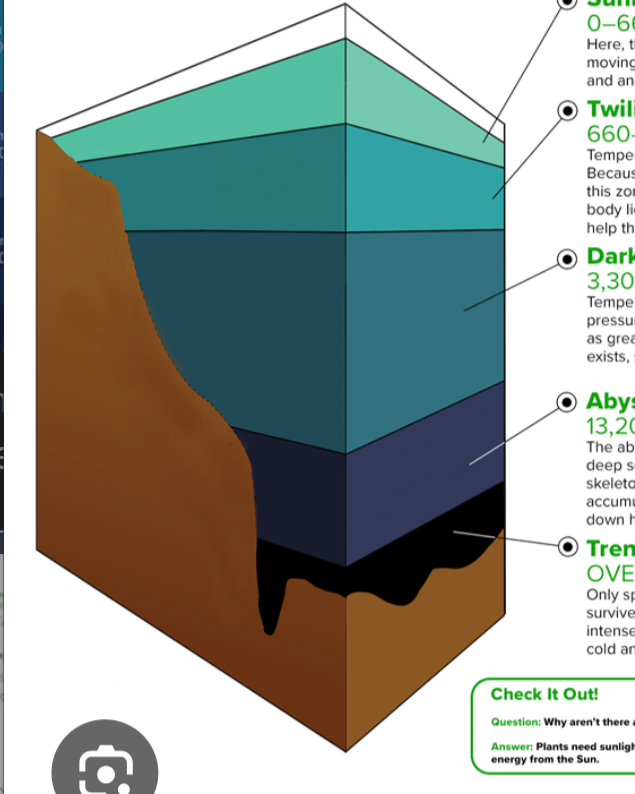
\includegraphics[width=\linewidth]{pptx_figures/image11.png}
    \caption{אזורי עומק אוקיינוס: טמפרטורה, לחץ ומליחות משתנים עם העומק,
             ומניעים שינויים במהירות הקול לאורך עמוד המים.}
  \end{subfigure}\hfill
  \begin{subfigure}[t]{0.45\textwidth}
    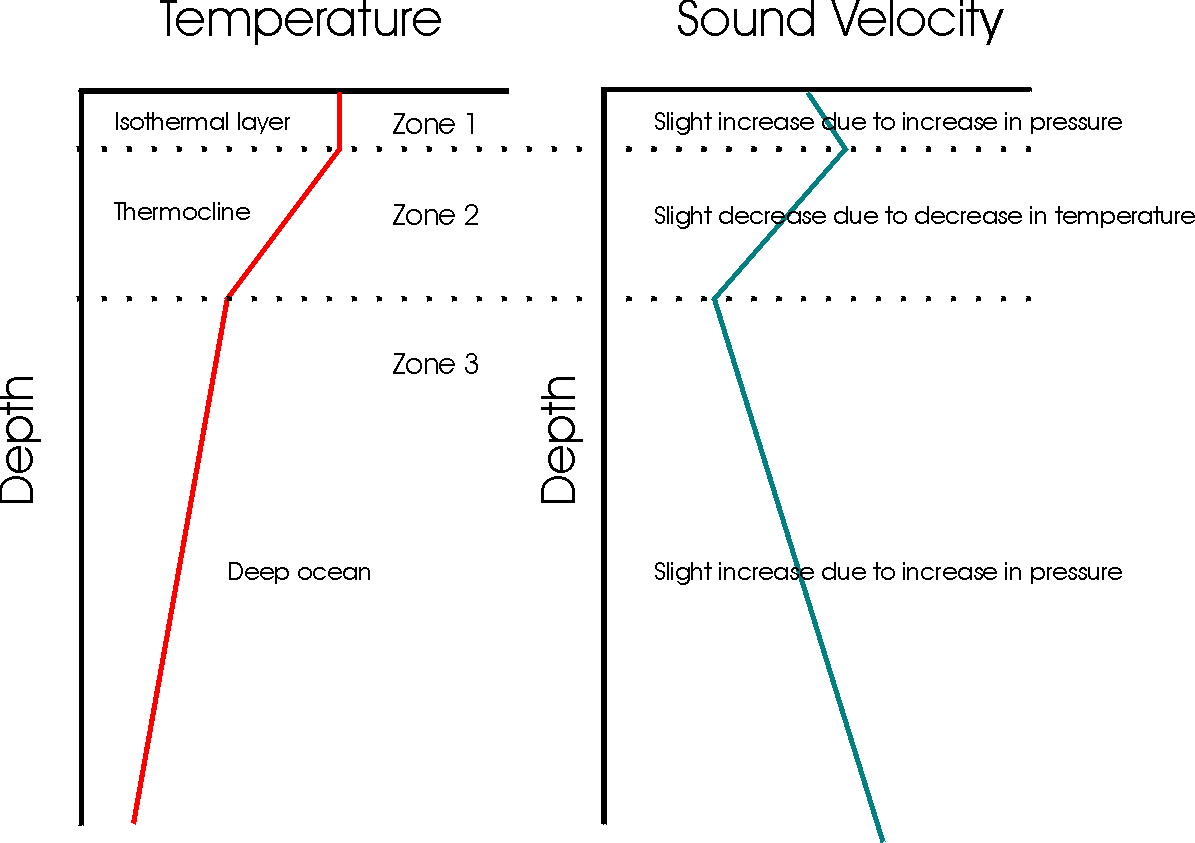
\includegraphics[width=\linewidth]{pptx_figures/image8.png}
    \caption{פרופיל SVP טיפוסי (קיץ): קביעת ציר ערוץ הקול (\textenglish{SOFAR})
             כנקודת מינימום סביב 1000~מ'.}
  \end{subfigure}
  \caption{הים כמדיום אקוסטי שכבתי: מבנה פרופיל SVP ואפקט ה-\textenglish{SOFAR}.}
  \label{fig:ocean_layers}
\end{figure}

% ─────────────────────────────────────────
\subsection{התפשטות גלים אקוסטיים ומודל \textenglish{Bellhop}}
\label{sec:bellhop}

\begin{english}
The acoustic field in the ocean is described by the Helmholtz equation in a
cylindrically symmetric ($r$-$z$) geometry:
\end{english}
\begin{equation}
  \nabla^2 p + k^2(r,z)\,p = -S(r,z), \quad k = \frac{2\pi f}{c(r,z)},
\end{equation}
\begin{english}
where $p$ is the complex pressure amplitude, $f$ is frequency, $c(r,z)$ is the
local sound speed, and $S$ is the source term.
Transmission loss is defined as:
\end{english}
\begin{equation}
  \TL(r,z) = -20\log_{10}\!\left(\frac{|p(r,z)|}{|p_{\mathrm{ref}}|}\right) \quad [\text{dB}].
\end{equation}
\begin{english}
\textenglish{Bellhop}~\cite{porter1987bellhop} solves this equation in the Gaussian
beam approximation: acoustic energy propagates along rays, each carrying a Gaussian
amplitude envelope that handles diffraction without the near-singularity of simple
geometric optics.
The model handles sea-floor reflections, surface reflections, and refraction through
the sound-speed gradient automatically.
\end{english}

\begin{figure}[H]
  \centering
  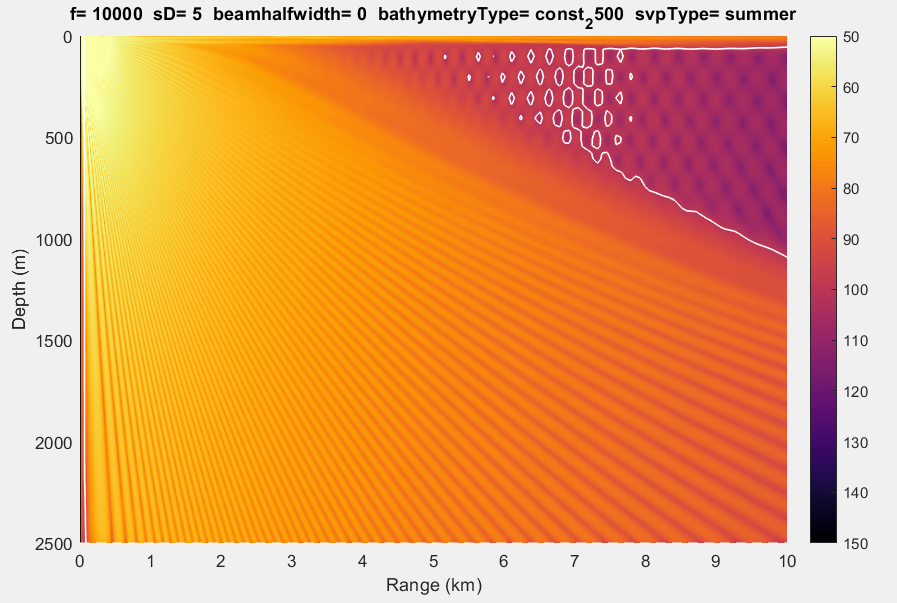
\includegraphics[width=0.80\textwidth]{pptx_figures/image7.png}
  \caption{\textenglish{Bellhop} כקופסה שחורה: כניסות (SVP, גיאומטריה, תדר, מאפייני קרקע)
           ויציאות (שדה TL, תרשים קרנים). הקרנים הגאוסיאניות מטפלות
           בהחזרות, שבירות ועדשות אקוסטיות.}
  \label{fig:bellhop_blackbox}
\end{figure}

% ─────────────────────────────────────────
\subsection{משוואת הסונאר וציון ההצלחה}
\label{sec:sonar_equation}

\begin{english}
The passive sonar equation links transmitter, medium, and receiver:
\end{english}
\begin{equation}
  \mathrm{SNR} = \mathrm{SL} - \TL - (\mathrm{NL} - \mathrm{DI})
\end{equation}
\begin{english}
Detection occurs when $\mathrm{SNR} > \mathrm{DT}$ (detection threshold).
Rearranging gives the \emph{Figure of Merit} (FOM):
\end{english}
\begin{equation}
  \mathrm{FOM} = \mathrm{SL} - \mathrm{NL} + \mathrm{DI} - \mathrm{DT}.
\end{equation}
\begin{english}
Detection is possible at a given $(r,z)$ pixel if and only if $\TL(r,z) < \mathrm{FOM}$.
In a stochastic environment, this becomes a probability:
\end{english}
\begin{equation}
  \Pshadow(\mathbf{x}) = P\!\bigl(\TL(\mathbf{x};\boldsymbol{\theta}) > \mathrm{FOM}\bigr).
\end{equation}
\begin{english}
This shadow probability $\Pshadow$ is the primary UQ output of interest.
\end{english}

% ─────────────────────────────────────────
\subsection{תופעות התפשטות: אזורי התכנסות והחזרות קרקע}
\label{sec:propagation_phenomena}

\begin{english}
Two acoustic propagation phenomena dominate at long range in deep water:
\end{english}
\begin{itemize}
  \item \begin{english}
          \textbf{Convergence zones (CZ)}: the sound-channel focusing mechanism
          produces periodic arcs of low TL (high energy) at multiples of the CZ range
          ($\sim$55\,km for a typical deep-water SVP).
          CZ position is highly sensitive to the near-surface SVP: a 5\% SVP
          perturbation can shift the CZ arc by $\pm$5--10\,km and change CZ gain
          by $\pm$5--10\,dB.
        \end{english}
  \item \begin{english}
          \textbf{Sea-floor reflections}: in shallow water and slope environments,
          acoustic energy bounces between the surface and the bottom, creating
          Lloyd's mirror interference patterns whose spatial period scales
          with $\lambda/2$ and which are highly sensitive to source depth $z_S$.
        \end{english}
\end{itemize}

\begin{figure}[H]
  \centering
  \begin{subfigure}[t]{0.48\textwidth}
    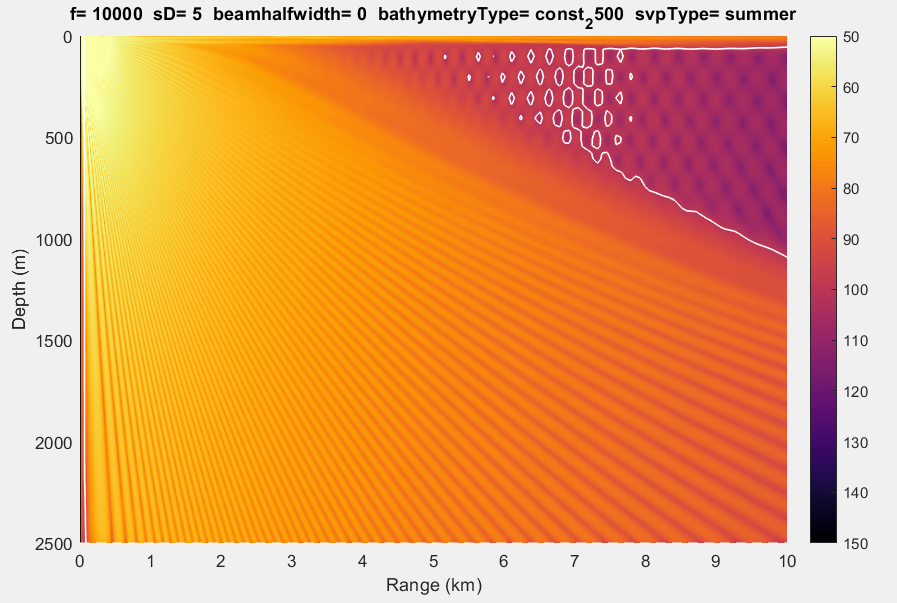
\includegraphics[width=\linewidth]{pptx_figures/image7.png}
    \caption{הגדרת הגיאומטריה}
  \end{subfigure}\hfill
  \begin{subfigure}[t]{0.48\textwidth}
    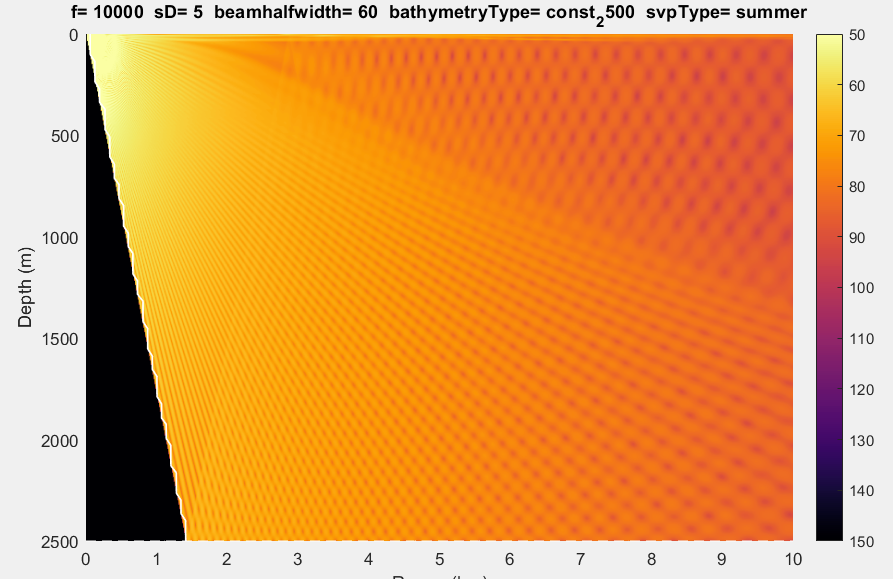
\includegraphics[width=\linewidth]{pptx_figures/image26.png}
    \caption{אזורי CZ ואזורי הצל}
  \end{subfigure}
  \caption{תופעות התפשטות אקוסטית בטווח ארוך: CZ והחזרות.}
  \label{fig:propagation}
\end{figure}

% ─────────────────────────────────────────
\subsection{ההרחבה הסטוכסטית: מדוע אי-ודאות חשובה}
\label{sec:stochastic}

\begin{english}
A single deterministic TL map $\TL(\mathbf{x};\boldsymbol{\theta}_0)$ computed at
the nominal parameter vector $\boldsymbol{\theta}_0 = (\bar{f},\bar{z}_S, \overline{\mathrm{SVP}})$
is insufficient for operational sonar planning for two reasons:

\begin{enumerate}
  \item \textbf{Measurement uncertainty.} The true environmental parameters are never
        known exactly; temperature profiles have $\pm$0.1--0.3$^\circ$C measurement
        uncertainty, source depths are uncertain by $\pm$5--10\,m, and carrier
        frequency can drift by $\pm$1\%{}.
  \item \textbf{Temporal variability.} The ocean SVP changes on time scales from hours
        (tidal mixing) to months (seasonal cycle); a TL map computed from a morning
        BT drop may be 5--10\,dB wrong by afternoon.
\end{enumerate}

The stochastic extension models each uncertain parameter as an independent Gaussian
random variable: $\theta_k \sim \mathcal{N}(\mu_k, \sigma_k^2)$ where $\sigma_k$
is a known percentage of $\mu_k$ (1\%, 5\%, or 10\% in our experiments).
The goal of UQ is to propagate these input distributions through the nonlinear
Bellhop operator to obtain the output distribution of TL at each pixel, and
thence the shadow probability $\Pshadow$.
\end{english}

% ─────────────────────────────────────────
\subsection{אימות אנליטי של \textenglish{Bellhop}}
\label{sec:analytical_validation}

\begin{english}
Before using \textenglish{Bellhop} as the stochastic forward model, we validated its
accuracy against two analytical solutions.
\end{english}

\subsubsection{מרחב חצי-אינסופי}

\begin{english}
For an isovelocity half-space (constant sound speed, pressure-release surface,
penetrable flat bottom), the exact TL is given by the Pekeris waveguide solution.
\textenglish{Bellhop} agrees to within $<$0.5\,dB over the full propagation range.
\end{english}

\begin{figure}[H]
  \centering
  \begin{subfigure}[t]{0.48\textwidth}
    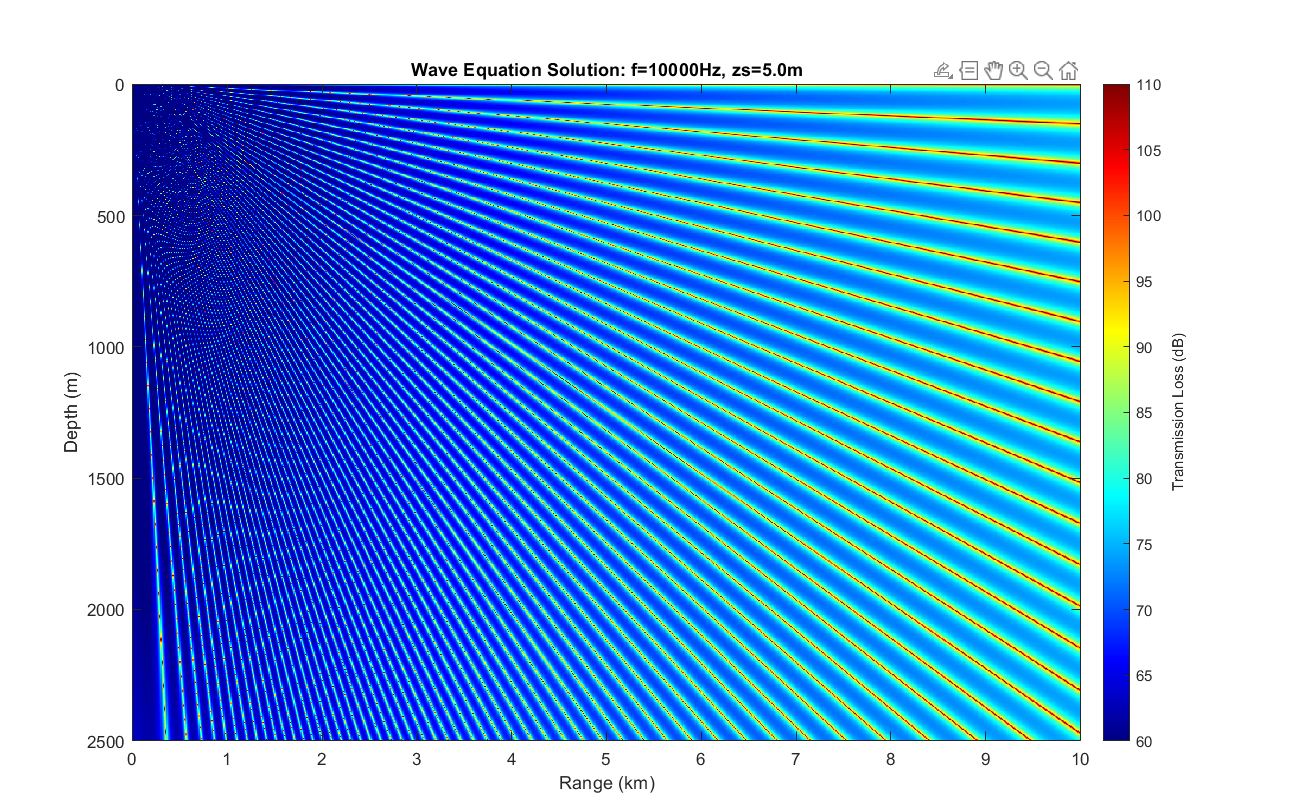
\includegraphics[width=\linewidth]{pptx_figures/image29.png}
    \caption{מרחב חצי-אינסופי}
  \end{subfigure}\hfill
  \begin{subfigure}[t]{0.48\textwidth}
    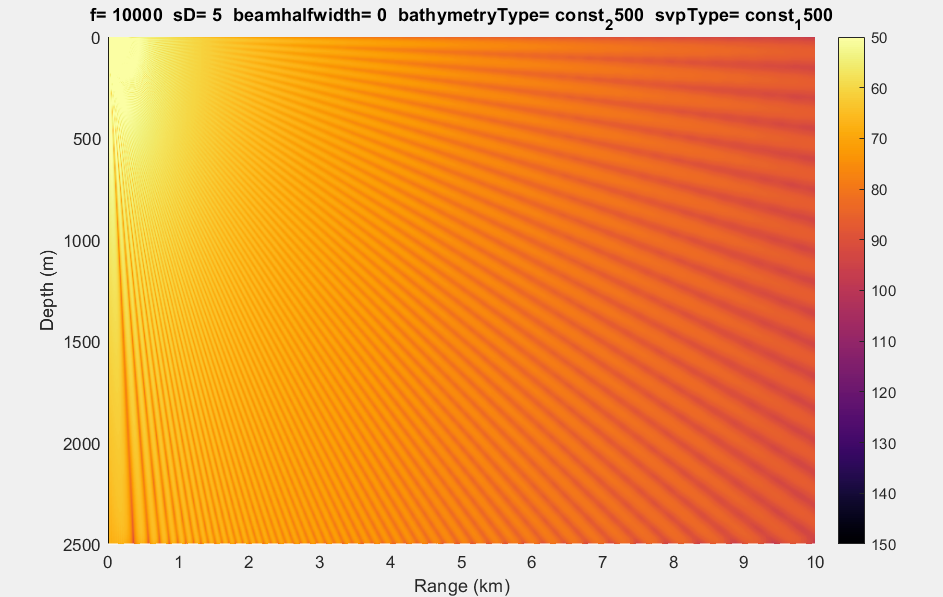
\includegraphics[width=\linewidth]{pptx_figures/image36.png}
    \caption{שגיאת TL לעומת ייחוס אנליטי}
  \end{subfigure}
  \caption{אימות \textenglish{Bellhop}: מרחב חצי-אינסופי (פתרון \textenglish{Pekeris}).}
  \label{fig:val_halfspace}
\end{figure}

\subsubsection{גלידה מהדי — מודים נורמליים}

\begin{english}
For a Pekeris waveguide with a rigid bottom boundary, the exact pressure field is
given by the normal-mode series.
\textenglish{Bellhop} matches the normal-mode solution with $<$1\,dB mean error at
frequencies $>$150\,Hz, confirming its adequacy as the forward model.
\end{english}

\begin{figure}[H]
  \centering
  \begin{subfigure}[t]{0.48\textwidth}
    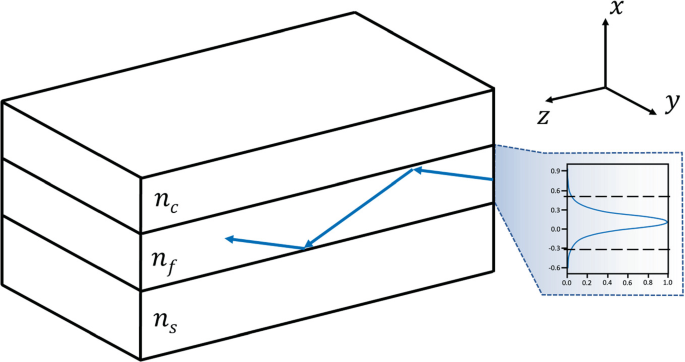
\includegraphics[width=\linewidth]{pptx_figures/image19.png}
    \caption{דיאגרמת גלידה מהדי (מודים)}
  \end{subfigure}\hfill
  \begin{subfigure}[t]{0.48\textwidth}
    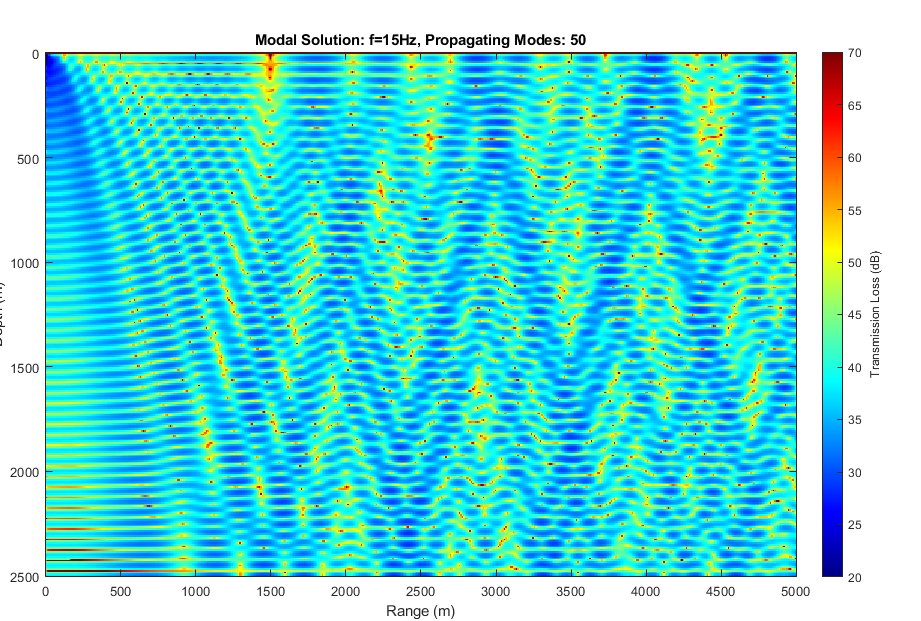
\includegraphics[width=\linewidth]{pptx_figures/image20.png}
    \caption{\textenglish{Bellhop} vs.\ מודים נורמליים}
  \end{subfigure}
  \caption{אימות \textenglish{Bellhop}: גלידה מהדי — מודים נורמליים.}
  \label{fig:val_waveguide}
\end{figure}

% ─────────────────────────────────────────
\subsection{רגישות TL לפרמטרים פיזיקליים}
\label{sec:sensitivity}

\begin{english}
Before performing full stochastic analysis, we visualise the qualitative sensitivity
of the TL field to each uncertain parameter by comparing TL maps computed at
$\theta_0 - \delta$, $\theta_0$, and $\theta_0 + \delta$.
SVP perturbation produces the most dramatic spatial redistribution of TL,
particularly at CZ boundaries.
Source depth and frequency produce more modest, qualitatively distinct patterns.
\end{english}

\begin{figure}[H]
  \centering
  \begin{subfigure}[t]{0.32\textwidth}
    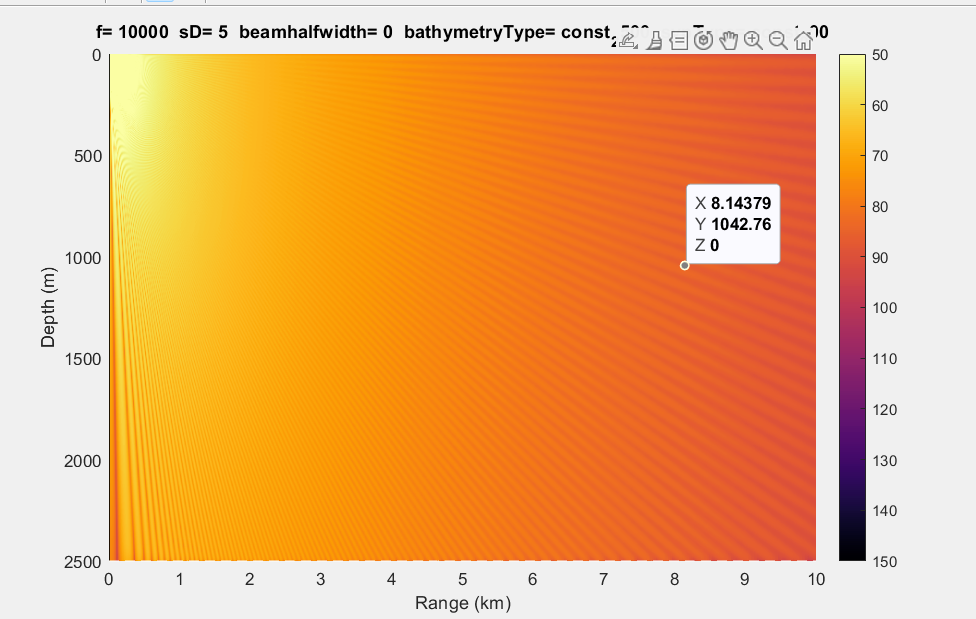
\includegraphics[width=\linewidth]{pptx_figures/image17.png}
    \caption{SVP $-\delta$}
  \end{subfigure}\hfill
  \begin{subfigure}[t]{0.32\textwidth}
    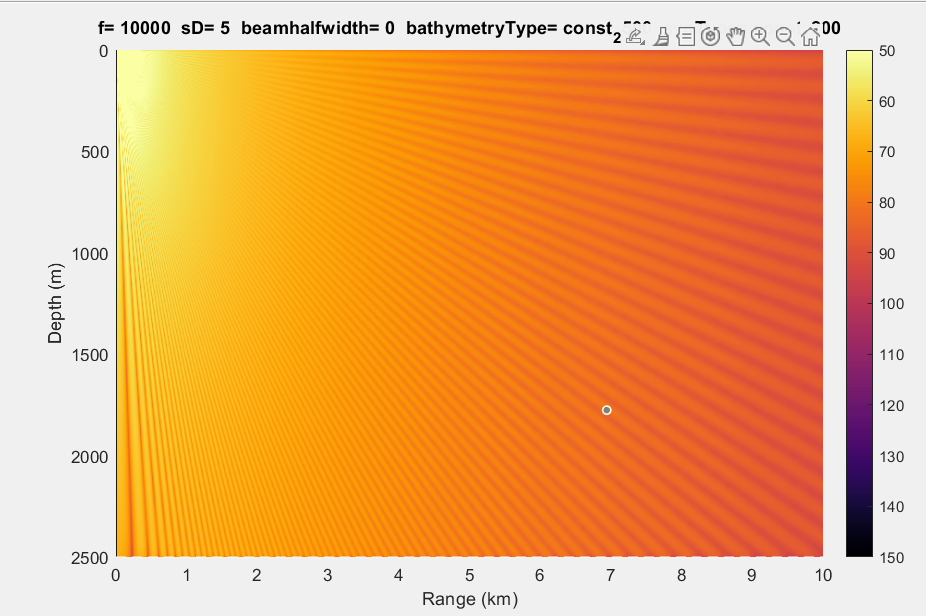
\includegraphics[width=\linewidth]{pptx_figures/image22.png}
    \caption{SVP $\mu$ (נומינלי)}
  \end{subfigure}\hfill
  \begin{subfigure}[t]{0.32\textwidth}
    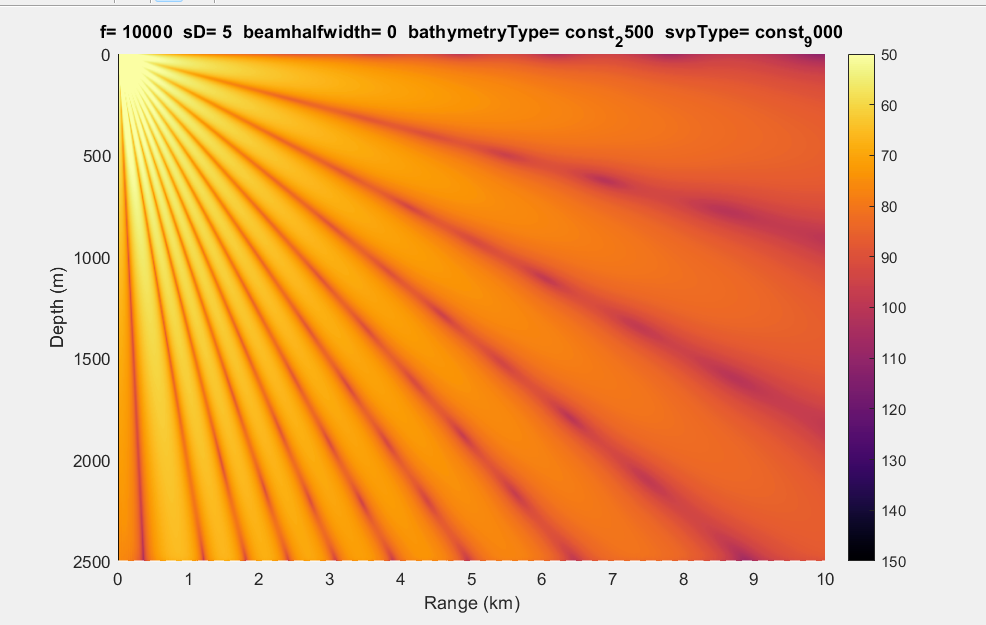
\includegraphics[width=\linewidth]{pptx_figures/image30.png}
    \caption{SVP $+\delta$}
  \end{subfigure}
  \caption{רגישות TL לשינויים ב-SVP: שלושה ערכי פרמטר.}
  \label{fig:svp_sensitivity}
\end{figure}

\begin{figure}[H]
  \centering
  \begin{subfigure}[t]{0.48\textwidth}
    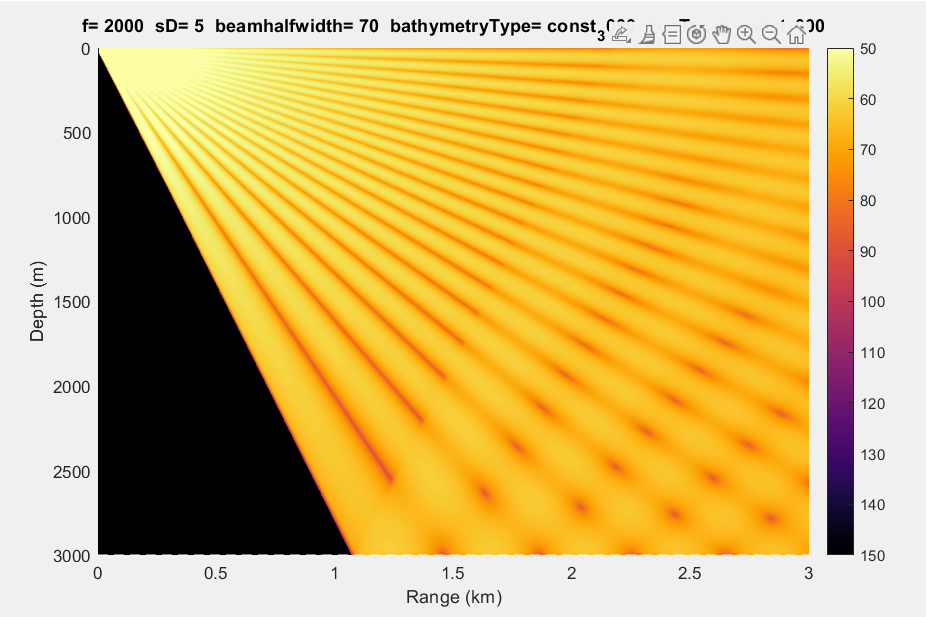
\includegraphics[width=\linewidth]{pptx_figures/image33.png}
    \caption{תדר נמוך}
  \end{subfigure}\hfill
  \begin{subfigure}[t]{0.48\textwidth}
    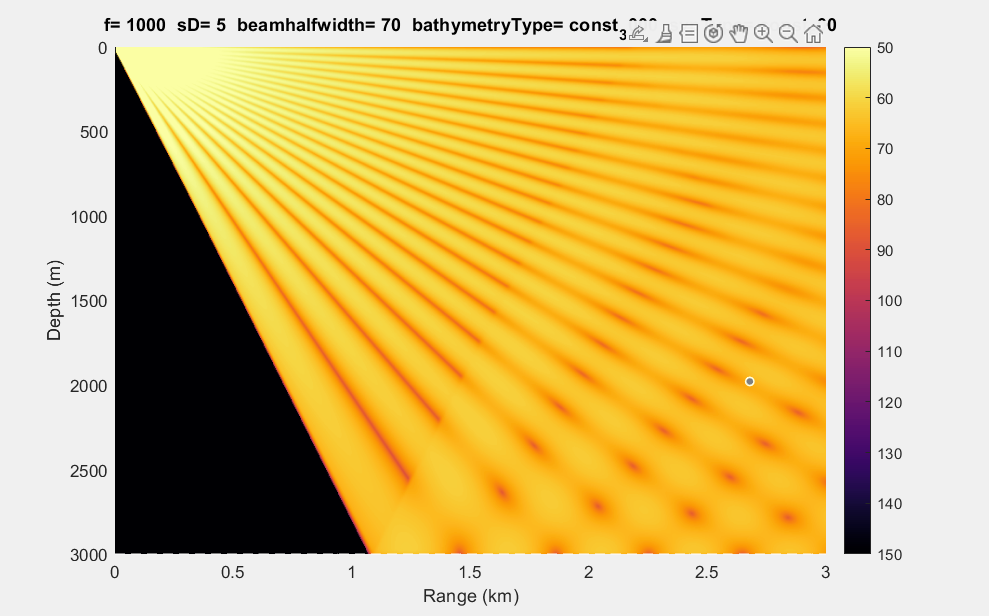
\includegraphics[width=\linewidth]{pptx_figures/image32.png}
    \caption{תדר גבוה}
  \end{subfigure}
  \caption{רגישות TL לשינויים בתדר.}
  \label{fig:freq_sensitivity}
\end{figure}

\begin{figure}[H]
  \centering
  \begin{subfigure}[t]{0.32\textwidth}
    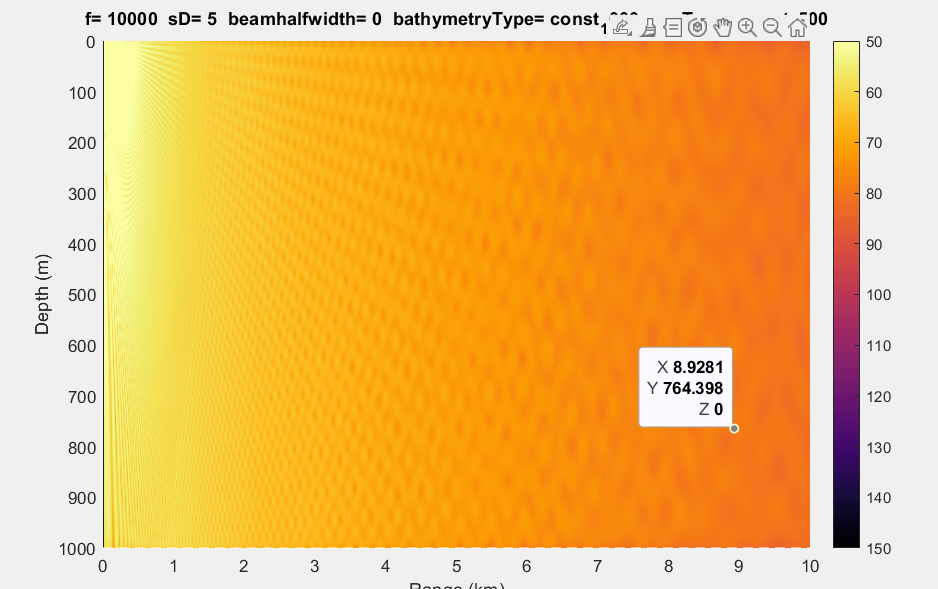
\includegraphics[width=\linewidth]{pptx_figures/image21.png}
    \caption{$z_S$ רדוד}
  \end{subfigure}\hfill
  \begin{subfigure}[t]{0.32\textwidth}
    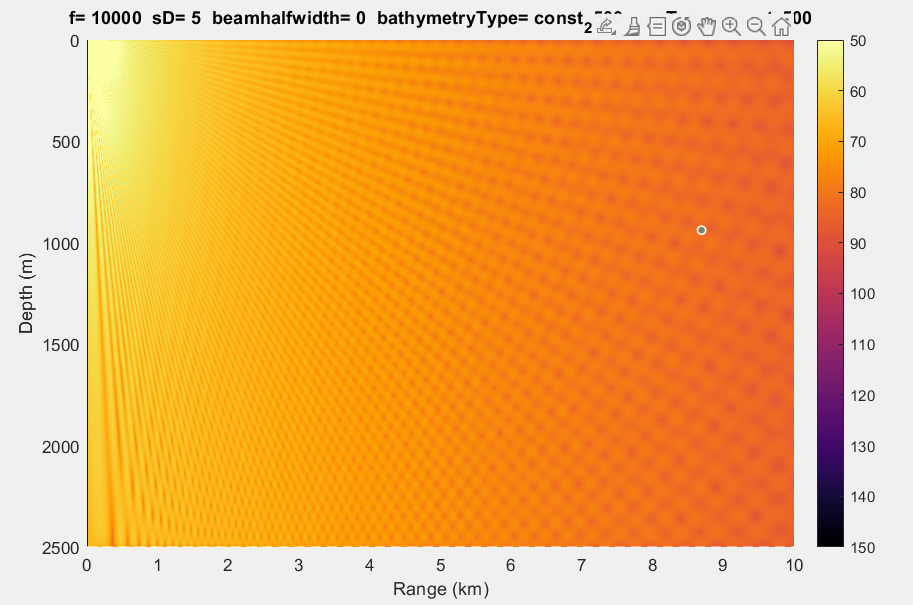
\includegraphics[width=\linewidth]{pptx_figures/image37.png}
    \caption{$z_S$ נומינלי}
  \end{subfigure}\hfill
  \begin{subfigure}[t]{0.32\textwidth}
    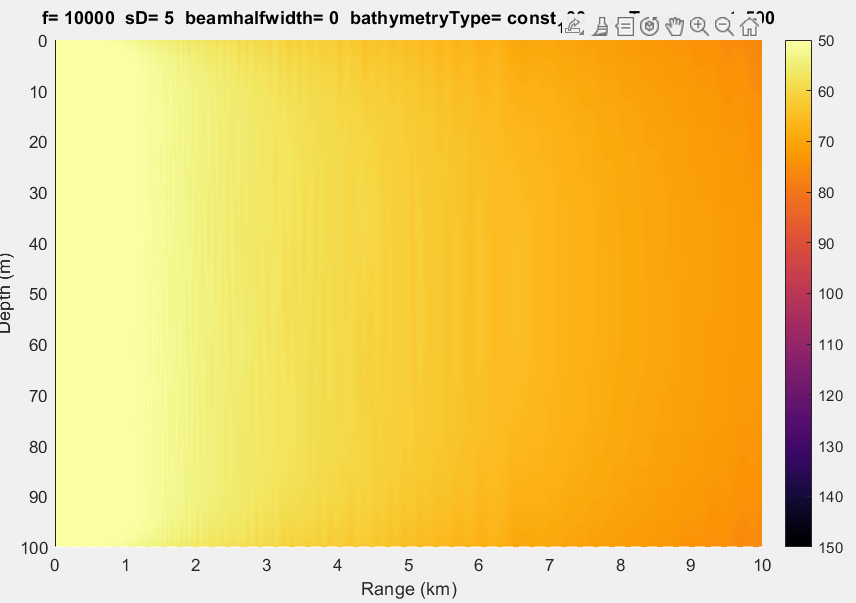
\includegraphics[width=\linewidth]{pptx_figures/image35.png}
    \caption{$z_S$ עמוק}
  \end{subfigure}
  \caption{רגישות TL לעומק מקור $z_S$.}
  \label{fig:zs_sensitivity}
\end{figure}

\begin{figure}[H]
  \centering
  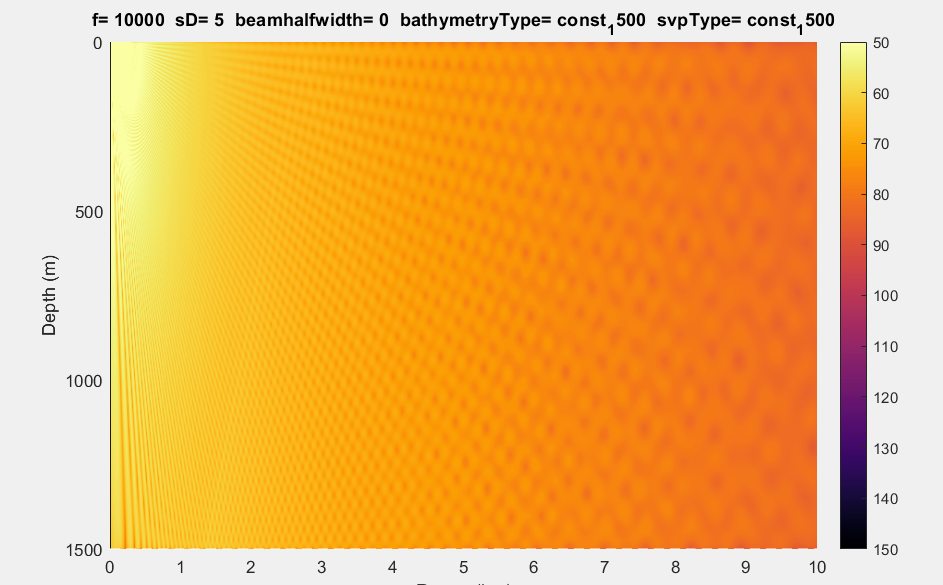
\includegraphics[width=0.60\textwidth]{pptx_figures/image24.png}
  \caption{משטר גלים: TL בתחום תדרים נמוכים מול גבוהים.}
  \label{fig:wavelength_regime}
\end{figure}

% ============================================================
%  2.  תוצאות
% ============================================================
\section{תוצאות}
\label{sec:results}

% ─────────────────────────────────────────
\subsection{גלריית תוצאות עיקריות}
\label{sec:gallery}

\begin{english}
The figures below show representative outputs from each UQ method for the deep-water /
Normal\,5\% scenario.
Each figure is discussed in detail in the corresponding subsection; the gallery is
structured so that each pair of maps can be compared side by side at full resolution.
\end{english}

\begin{figure}[H]
  \centering
  \begin{subfigure}[t]{0.48\textwidth}
    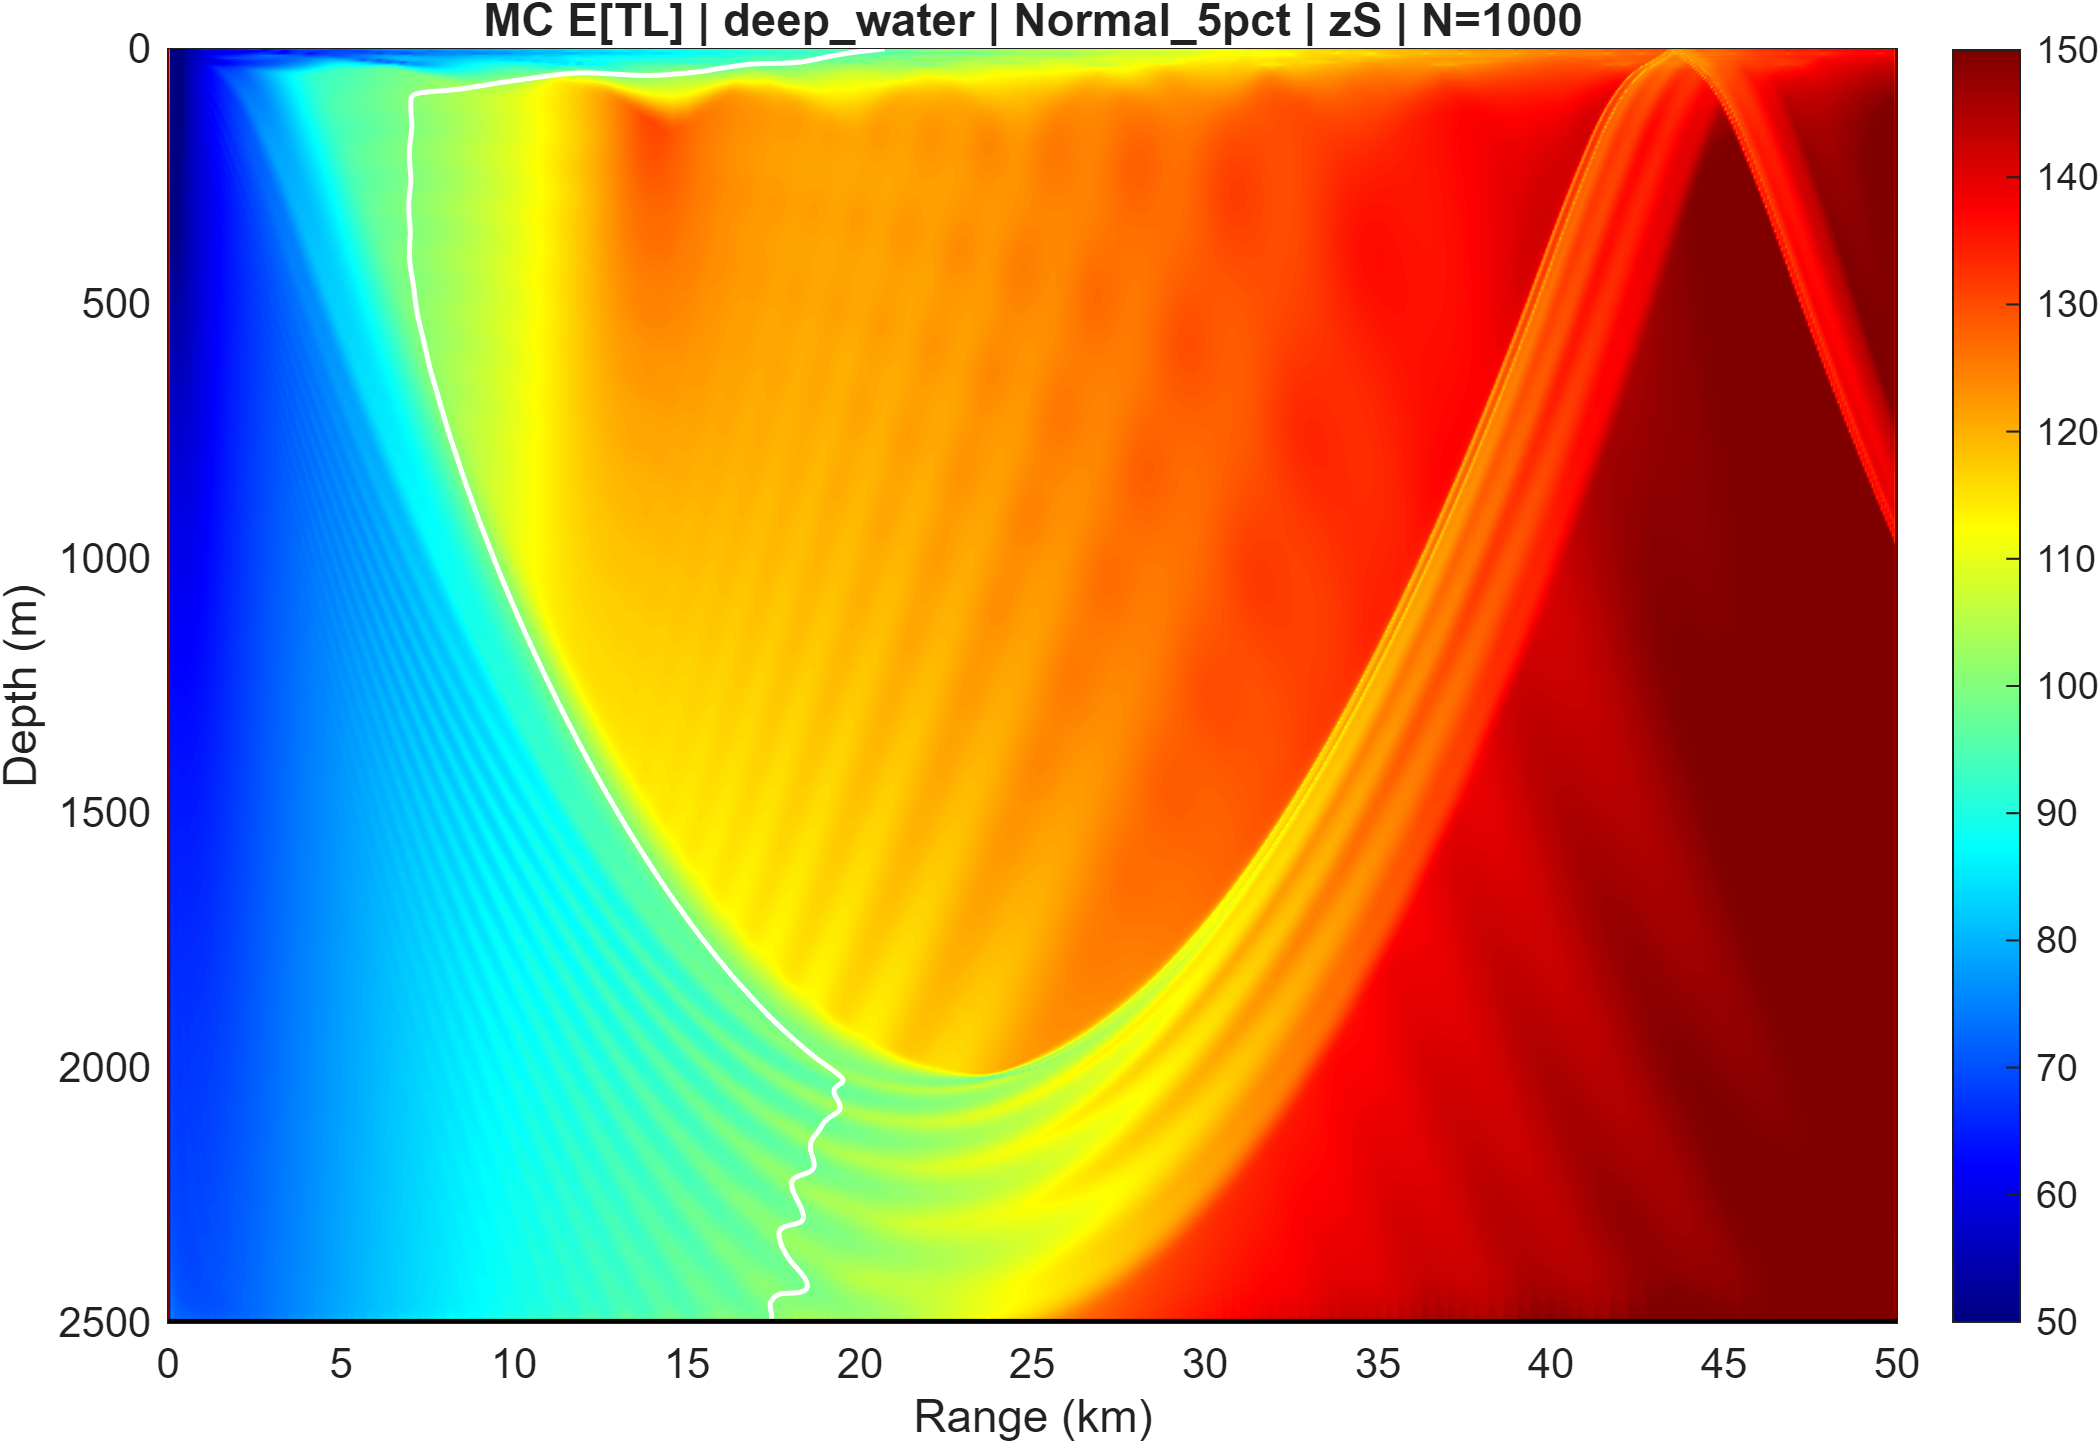
\includegraphics[width=\linewidth]{deep_water/Normal_5pct/figures/TL_zS.png}
    \caption{\textbf{ממוצע TL MC} תחת הפרעה ב-$z_S$ (נורמלי 5\%{}).
             כחול = TL נמוך (אות חזק); אדום = TL גבוה (אזור צל).
             קשת ה-CZ ב-$\sim$55~ק"מ נראית בברור.}
  \end{subfigure}\hfill
  \begin{subfigure}[t]{0.48\textwidth}
    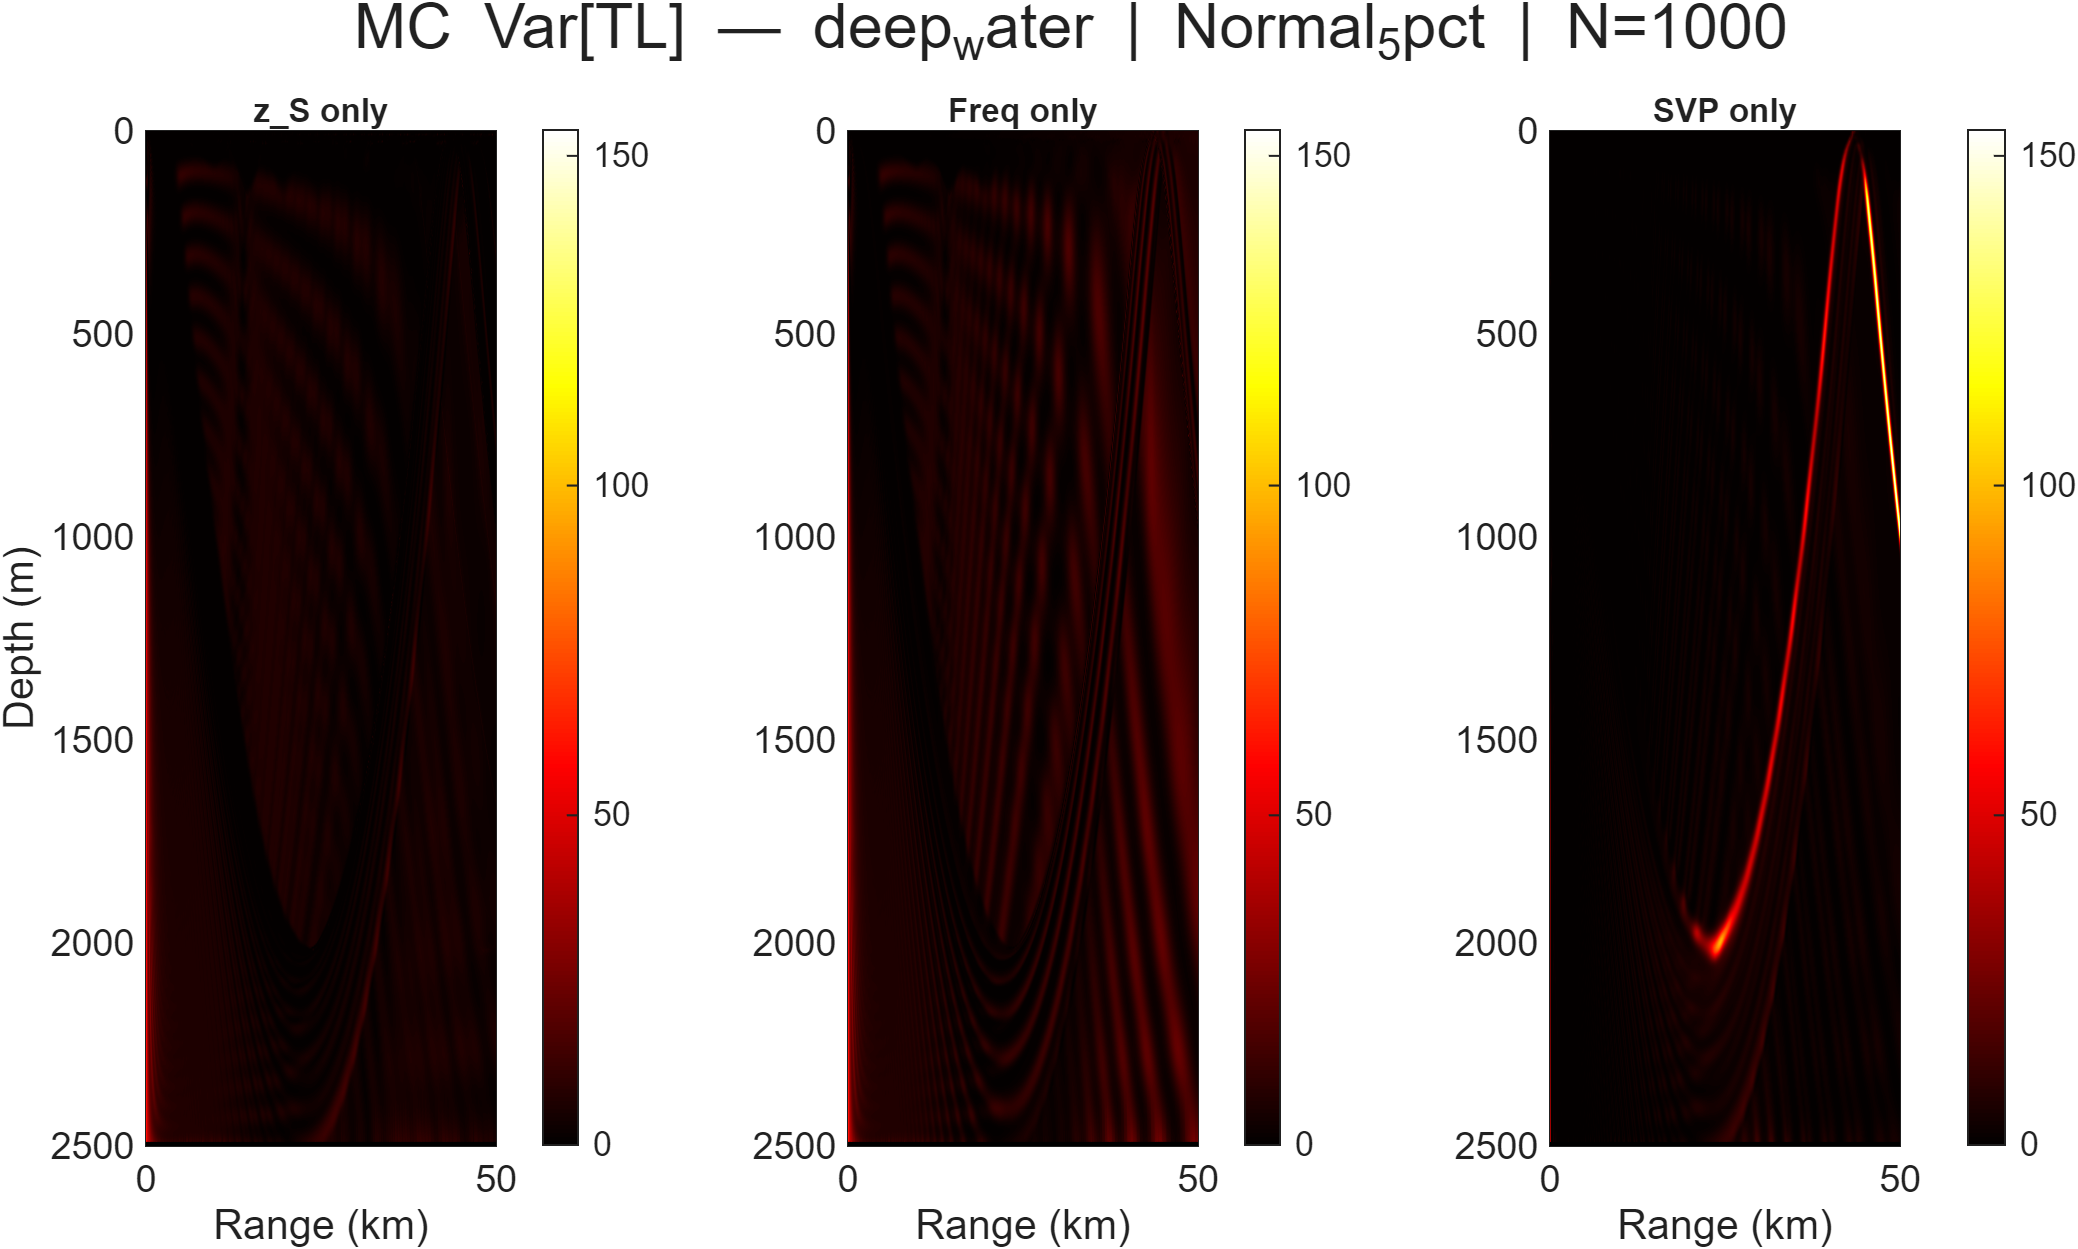
\includegraphics[width=\linewidth]{deep_water/Normal_5pct/figures/combined_Var.png}
    \caption{\textbf{מפות שונות MC} לשלושת הפרמטרים האי-ודאיים
             (\textenglish{freq, $z_S$, SVP}), בסקאלת צבע משותפת.
             SVP מייצר שונות מרחבית הטרוגנית ביותר.}
  \end{subfigure}
  \caption{מפות ייחוס MC למים עמוקים / נורמלי 5\%{}.
           שמאל: ממוצע $\EX[\TL]$ תחת הפרעת עומק מקור.
           ימין: שונות $\Var[\TL]$ לכל הפרמטרים.}
  \label{fig:gallery_mc}
\end{figure}

\begin{figure}[H]
  \centering
  \begin{subfigure}[t]{0.48\textwidth}
    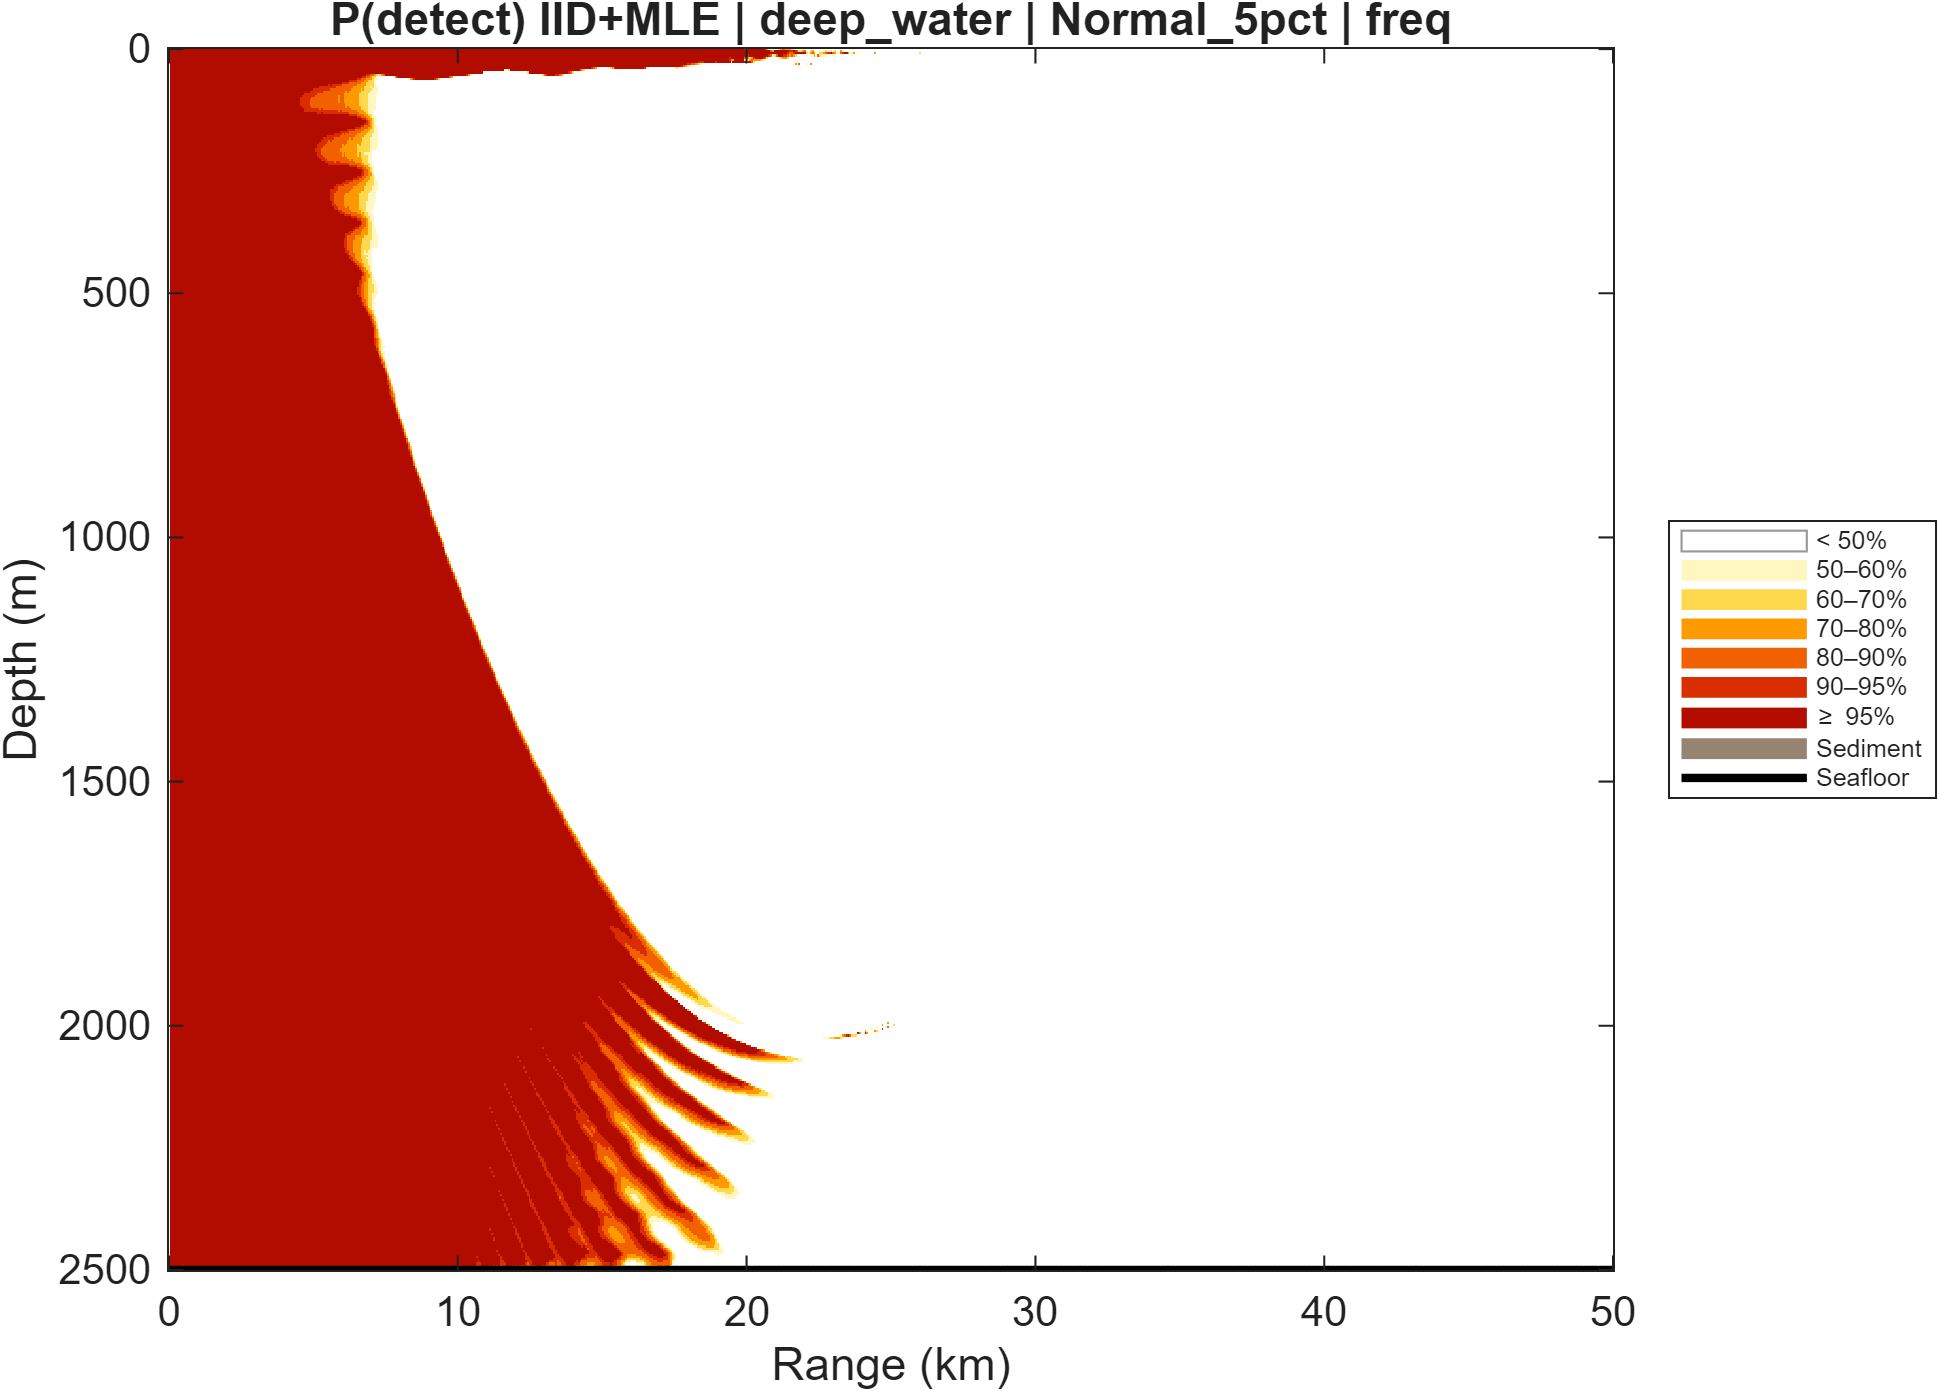
\includegraphics[width=\linewidth]{deep_water/Normal_5pct/figures/detect_mle_freq.png}
    \caption{\textbf{הסתברות צל מ-LN3 MLE} (הפרעת תדר).
             $P(\TL > \mathrm{FOM})$ בכל פיקסל, עוקפת את הצורך במדגם MC גדול.}
  \end{subfigure}\hfill
  \begin{subfigure}[t]{0.48\textwidth}
    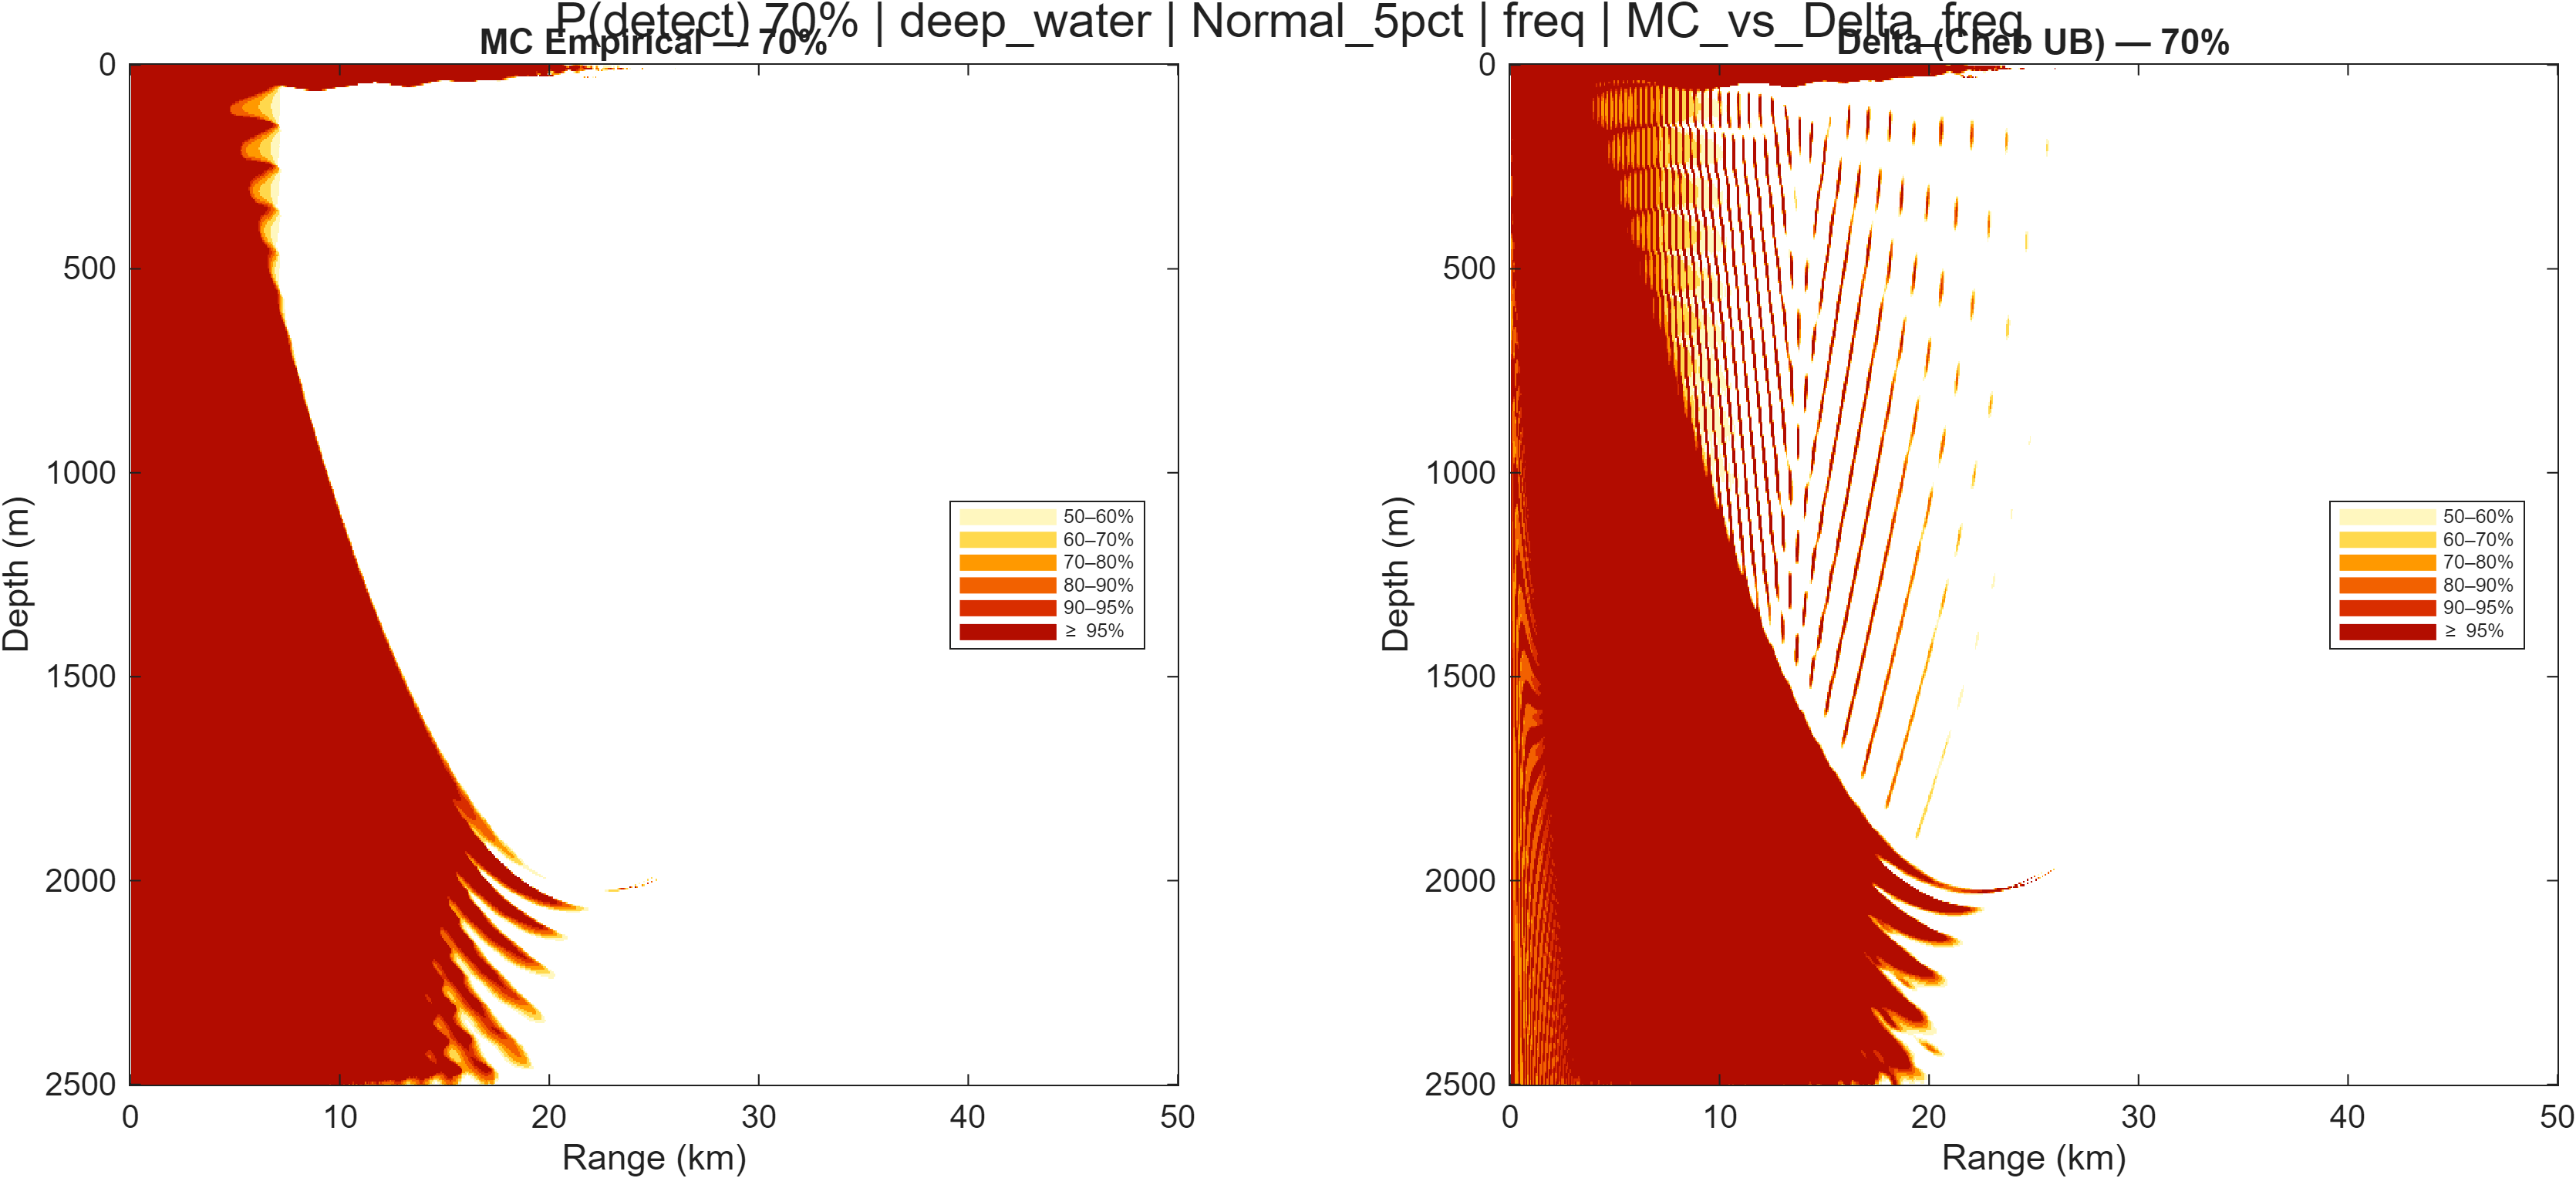
\includegraphics[width=\linewidth]{deep_water/Normal_5pct/figures/shadow_70_MC_vs_Delta_freq.png}
    \caption{\textbf{השוואת MC vs.\ Delta} להסתברות צל (הפרעת תדר).
             חצי שמאל: MC אמפירי; חצי ימין: קירוב $\Delta$-LN3.
             הסכמה קרובה מאשרת את $\Delta$ בתרחיש מים עמוקים.}
  \end{subfigure}
  \caption{מפות הסתברות גילוי עבור מים עמוקים / נורמלי 5\%{} / תדר.
           שמאל: הסתברות צל LN3-MLE. ימין: השוואת MC vs.\ Delta.}
  \label{fig:gallery_shadow}
\end{figure}

\begin{figure}[H]
  \centering
  \begin{subfigure}[t]{0.48\textwidth}
    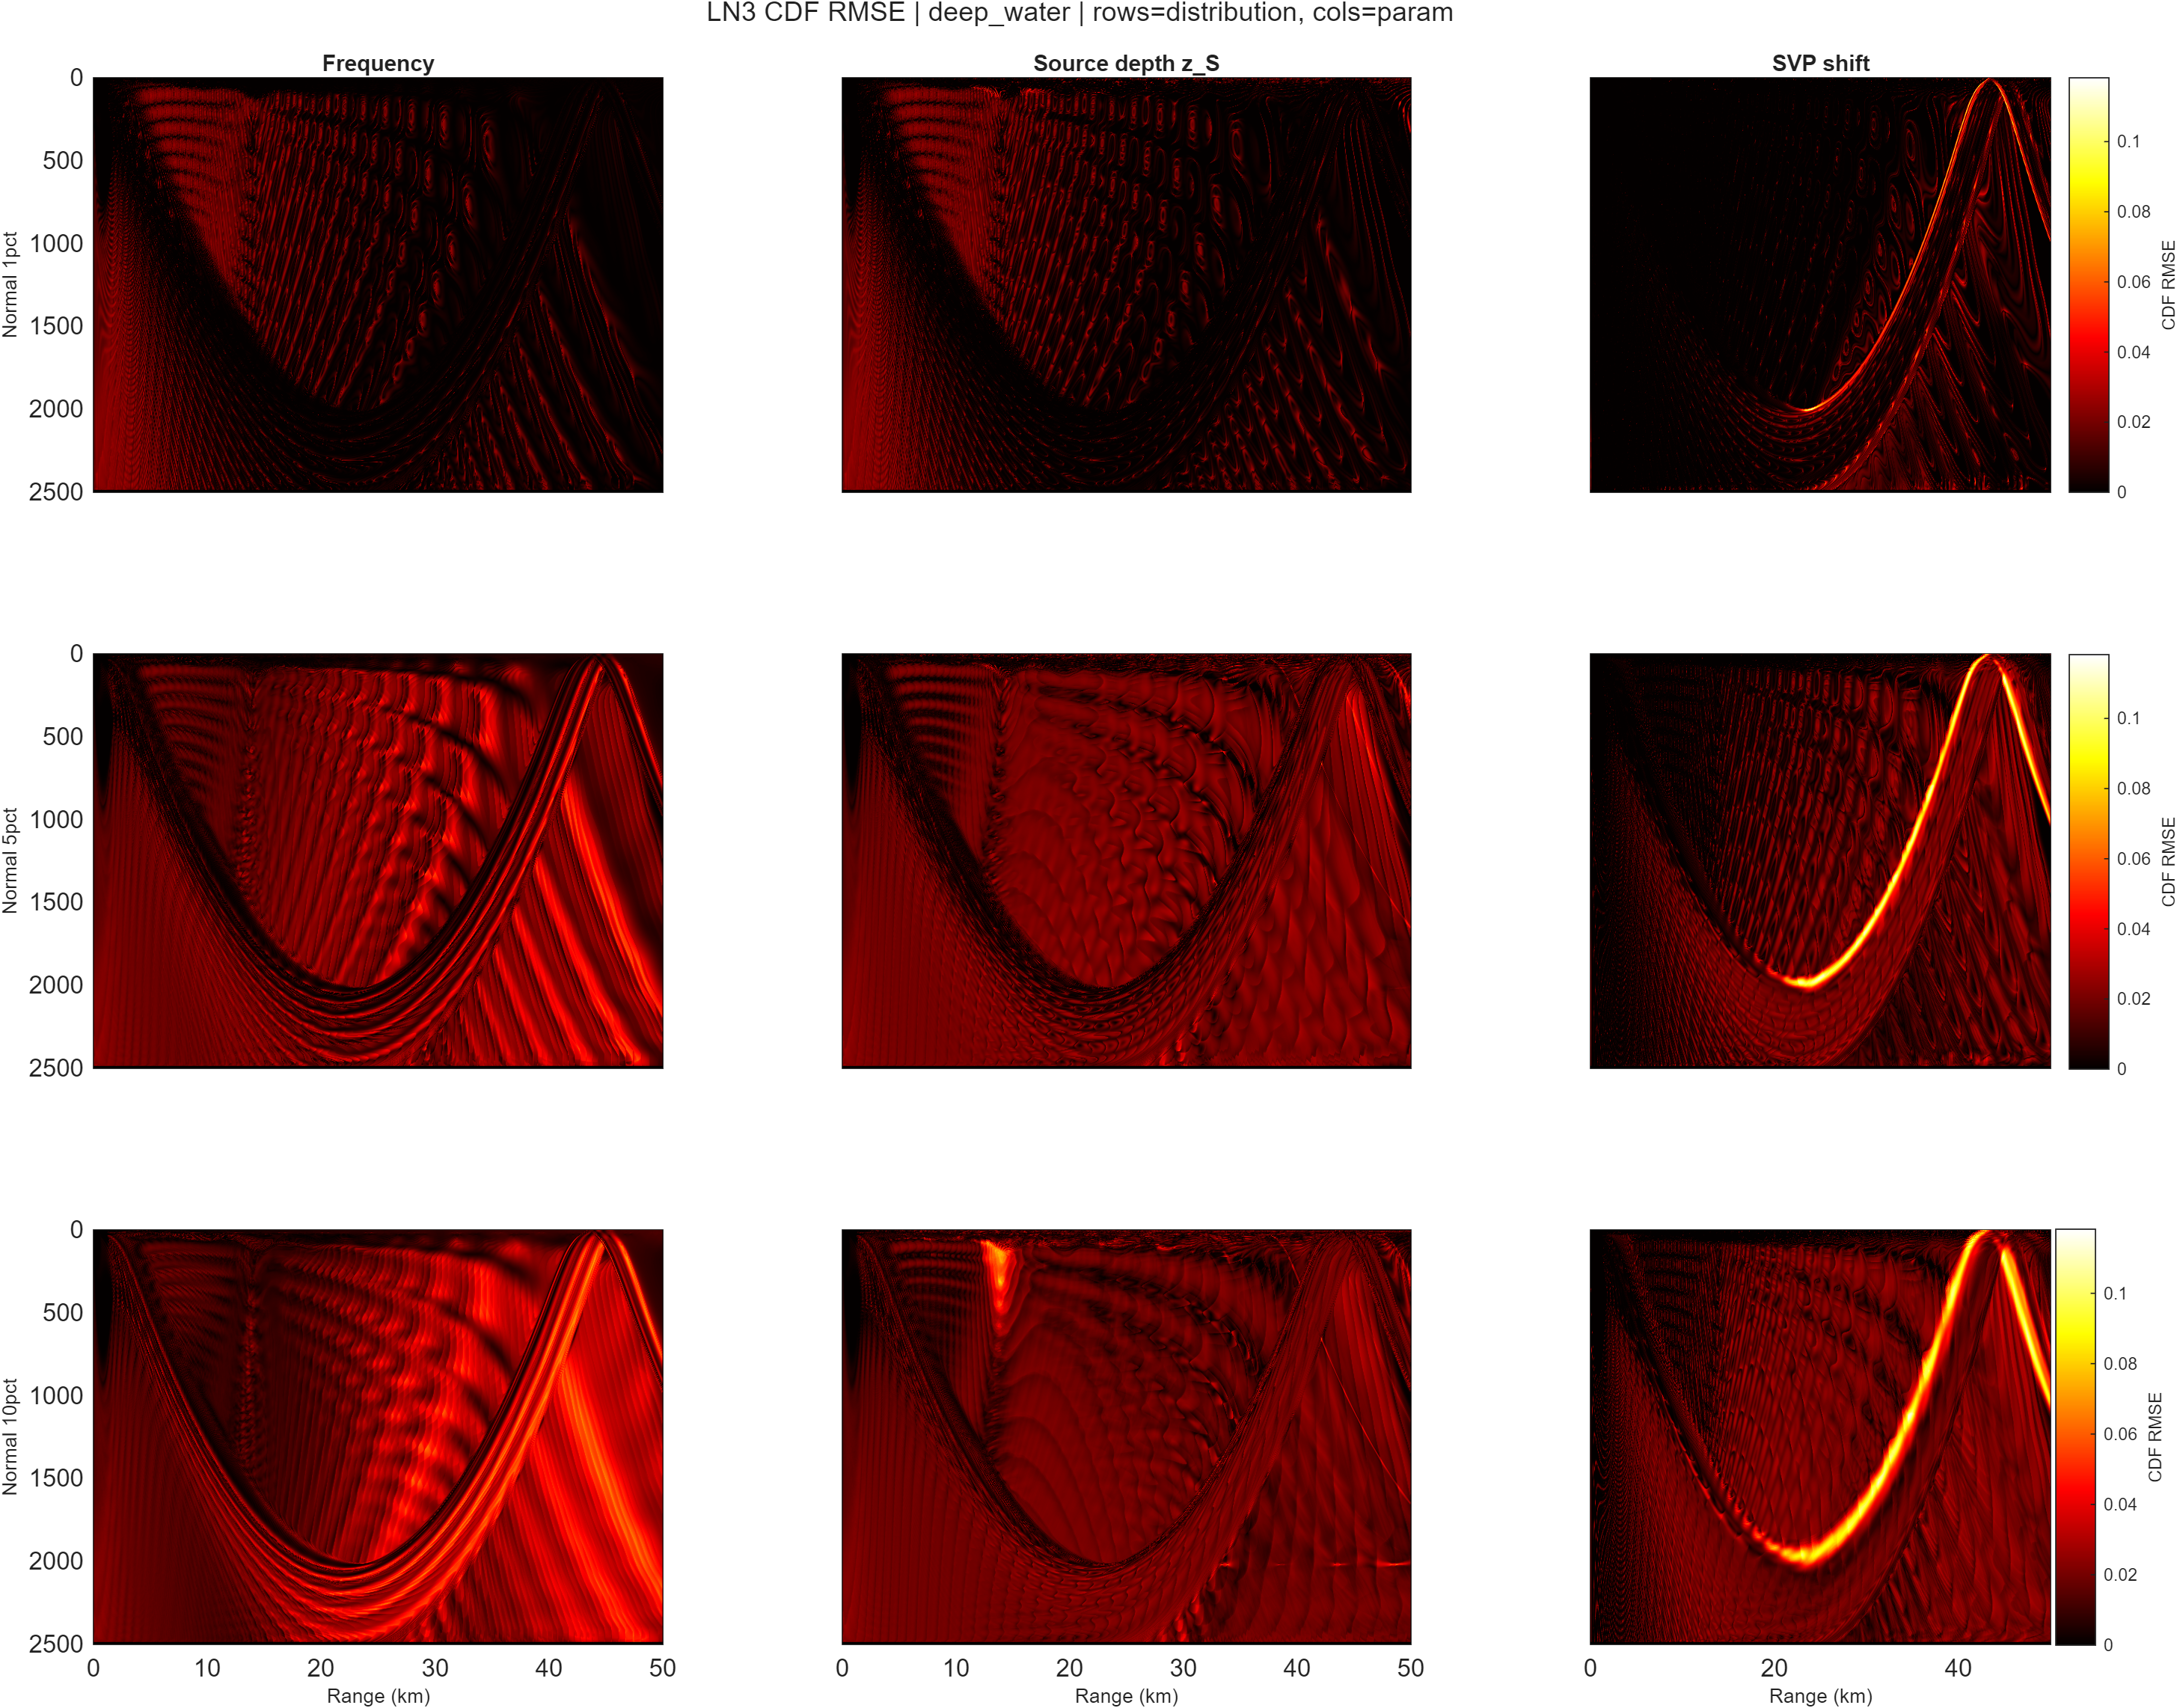
\includegraphics[width=\linewidth]{deep_water/figures/LN3_RMSE_all.png}
    \caption{\textbf{מפת RMSE של CDF ב-LN3} לכל ההתפלגויות והפרמטרים.
             שורות: נורמלי 1\%{}/5\%{}/10\%{}.
             עמודות: \textenglish{freq, $z_S$, SVP}.
             כהה = התאמה טובה; בהיר = התאמה גרועה.}
  \end{subfigure}\hfill
  \begin{subfigure}[t]{0.48\textwidth}
    
\includegraphics[width=\linewidth]{deep_water/Normal_5pct/figures/pce_order_relevance.png}
    \caption{\textbf{עקומת רלוונטיות סדר PCE} למים עמוקים / נורמלי 5\%{}.
             כל עקומה עולה מ-0\%{} ל-100\%{} בסדר האופטימלי $K^*$.
             שלושת הפרמטרים דורשים התפשטויות מסדר בינוני.}
  \end{subfigure}
  \caption{איכות התאמת LN3 ובחירת סדר PCE למים עמוקים / נורמלי 5\%{}.}
  \label{fig:gallery_ln3_pce}
\end{figure}

\begin{figure}[H]
  \centering
  \begin{subfigure}[t]{0.48\textwidth}
    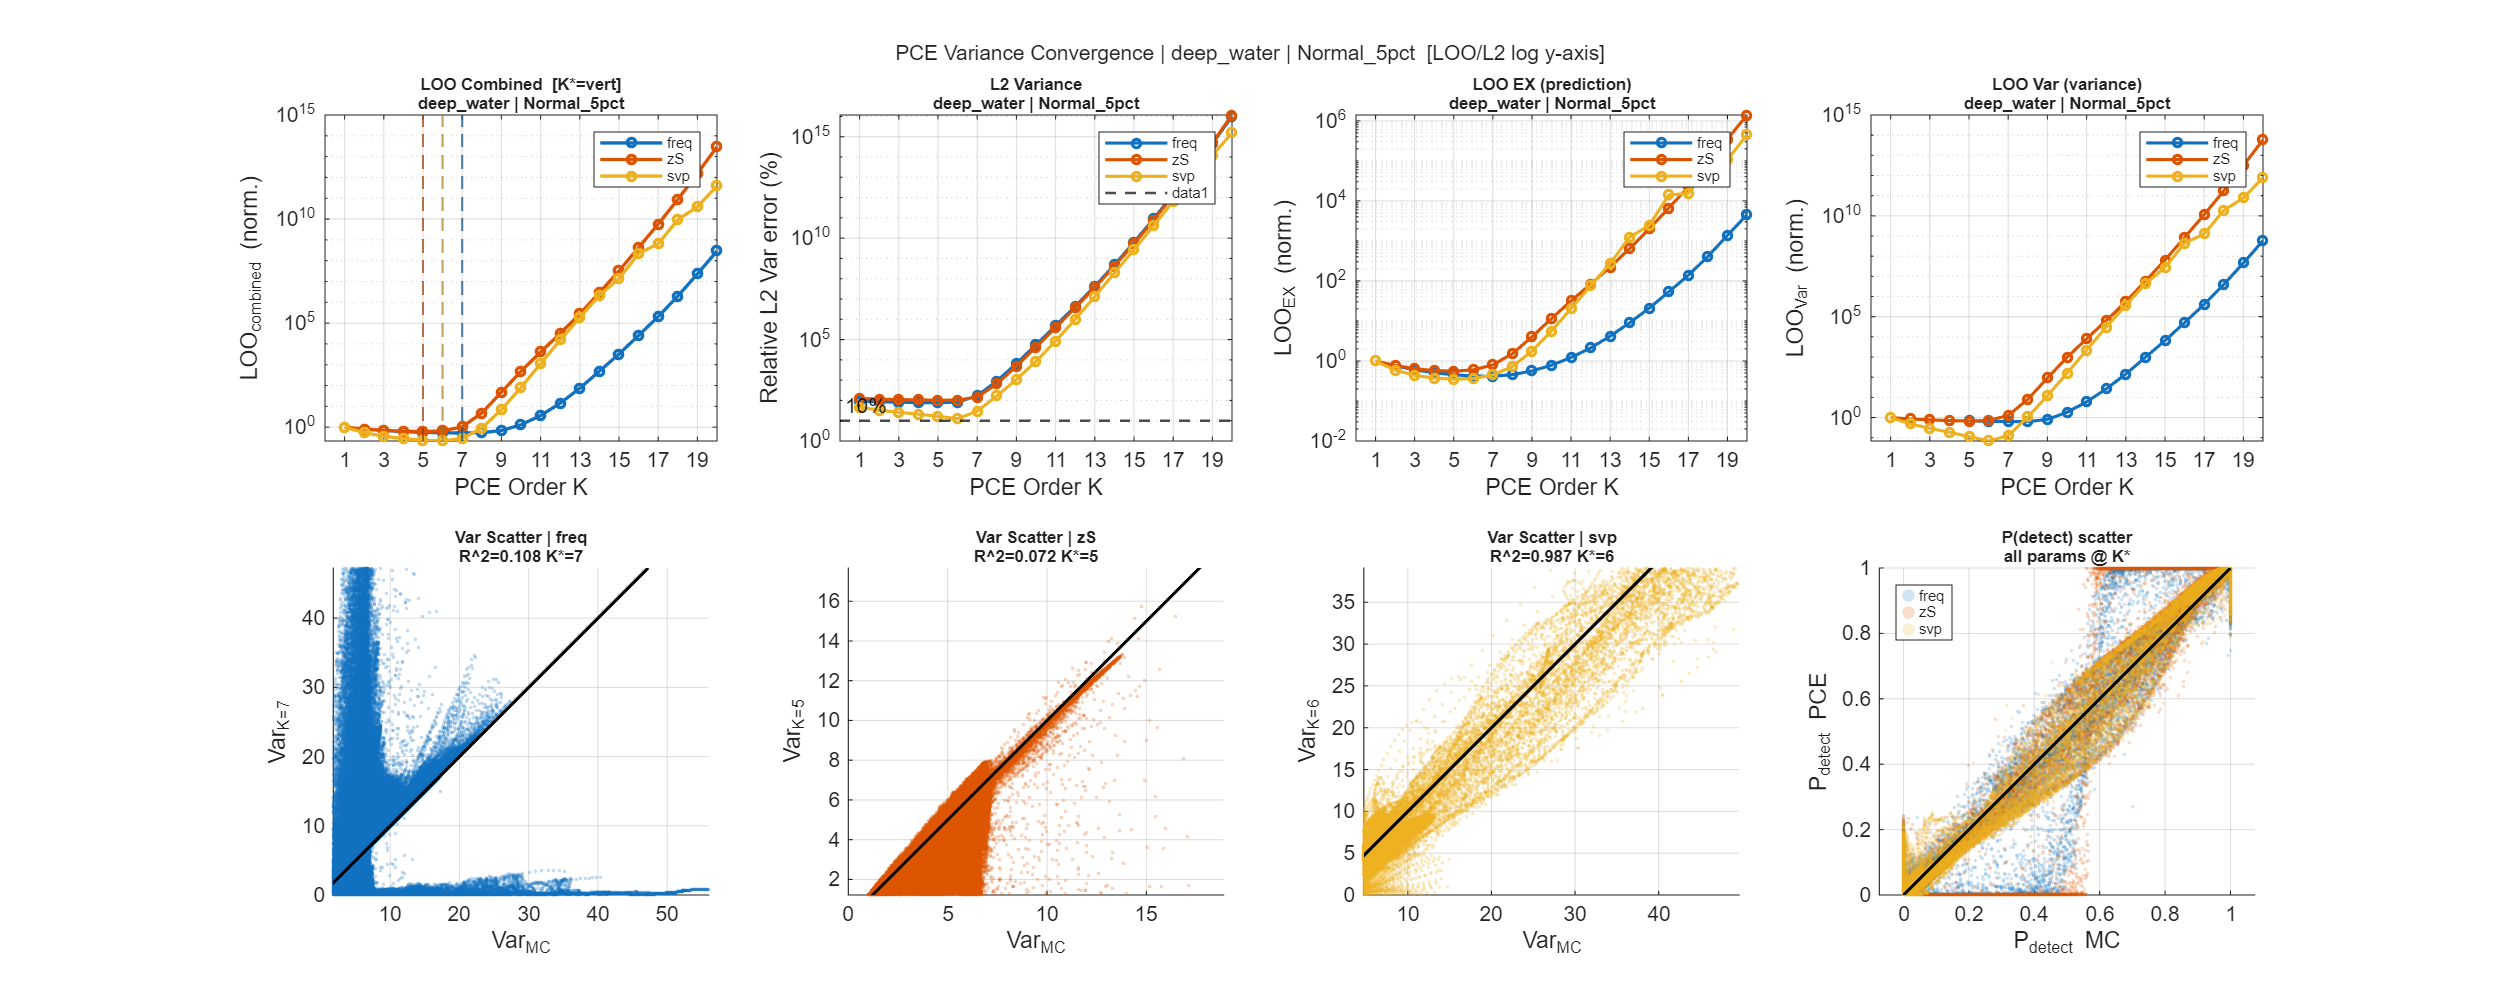
\includegraphics[width=\linewidth]{deep_water/Normal_5pct/figures/pce_convergence_deep_water_Normal_5pct.png}
    \caption{\textbf{התכנסות שגיאת L2 PCE} (מים עמוקים / נורמלי 5\%{}).
             כל קו הוא פרמטר אי-ודאי אחד.
             קו מקווקוו: סף 10\%{}.}
  \end{subfigure}\hfill
  \begin{subfigure}[t]{0.48\textwidth}
    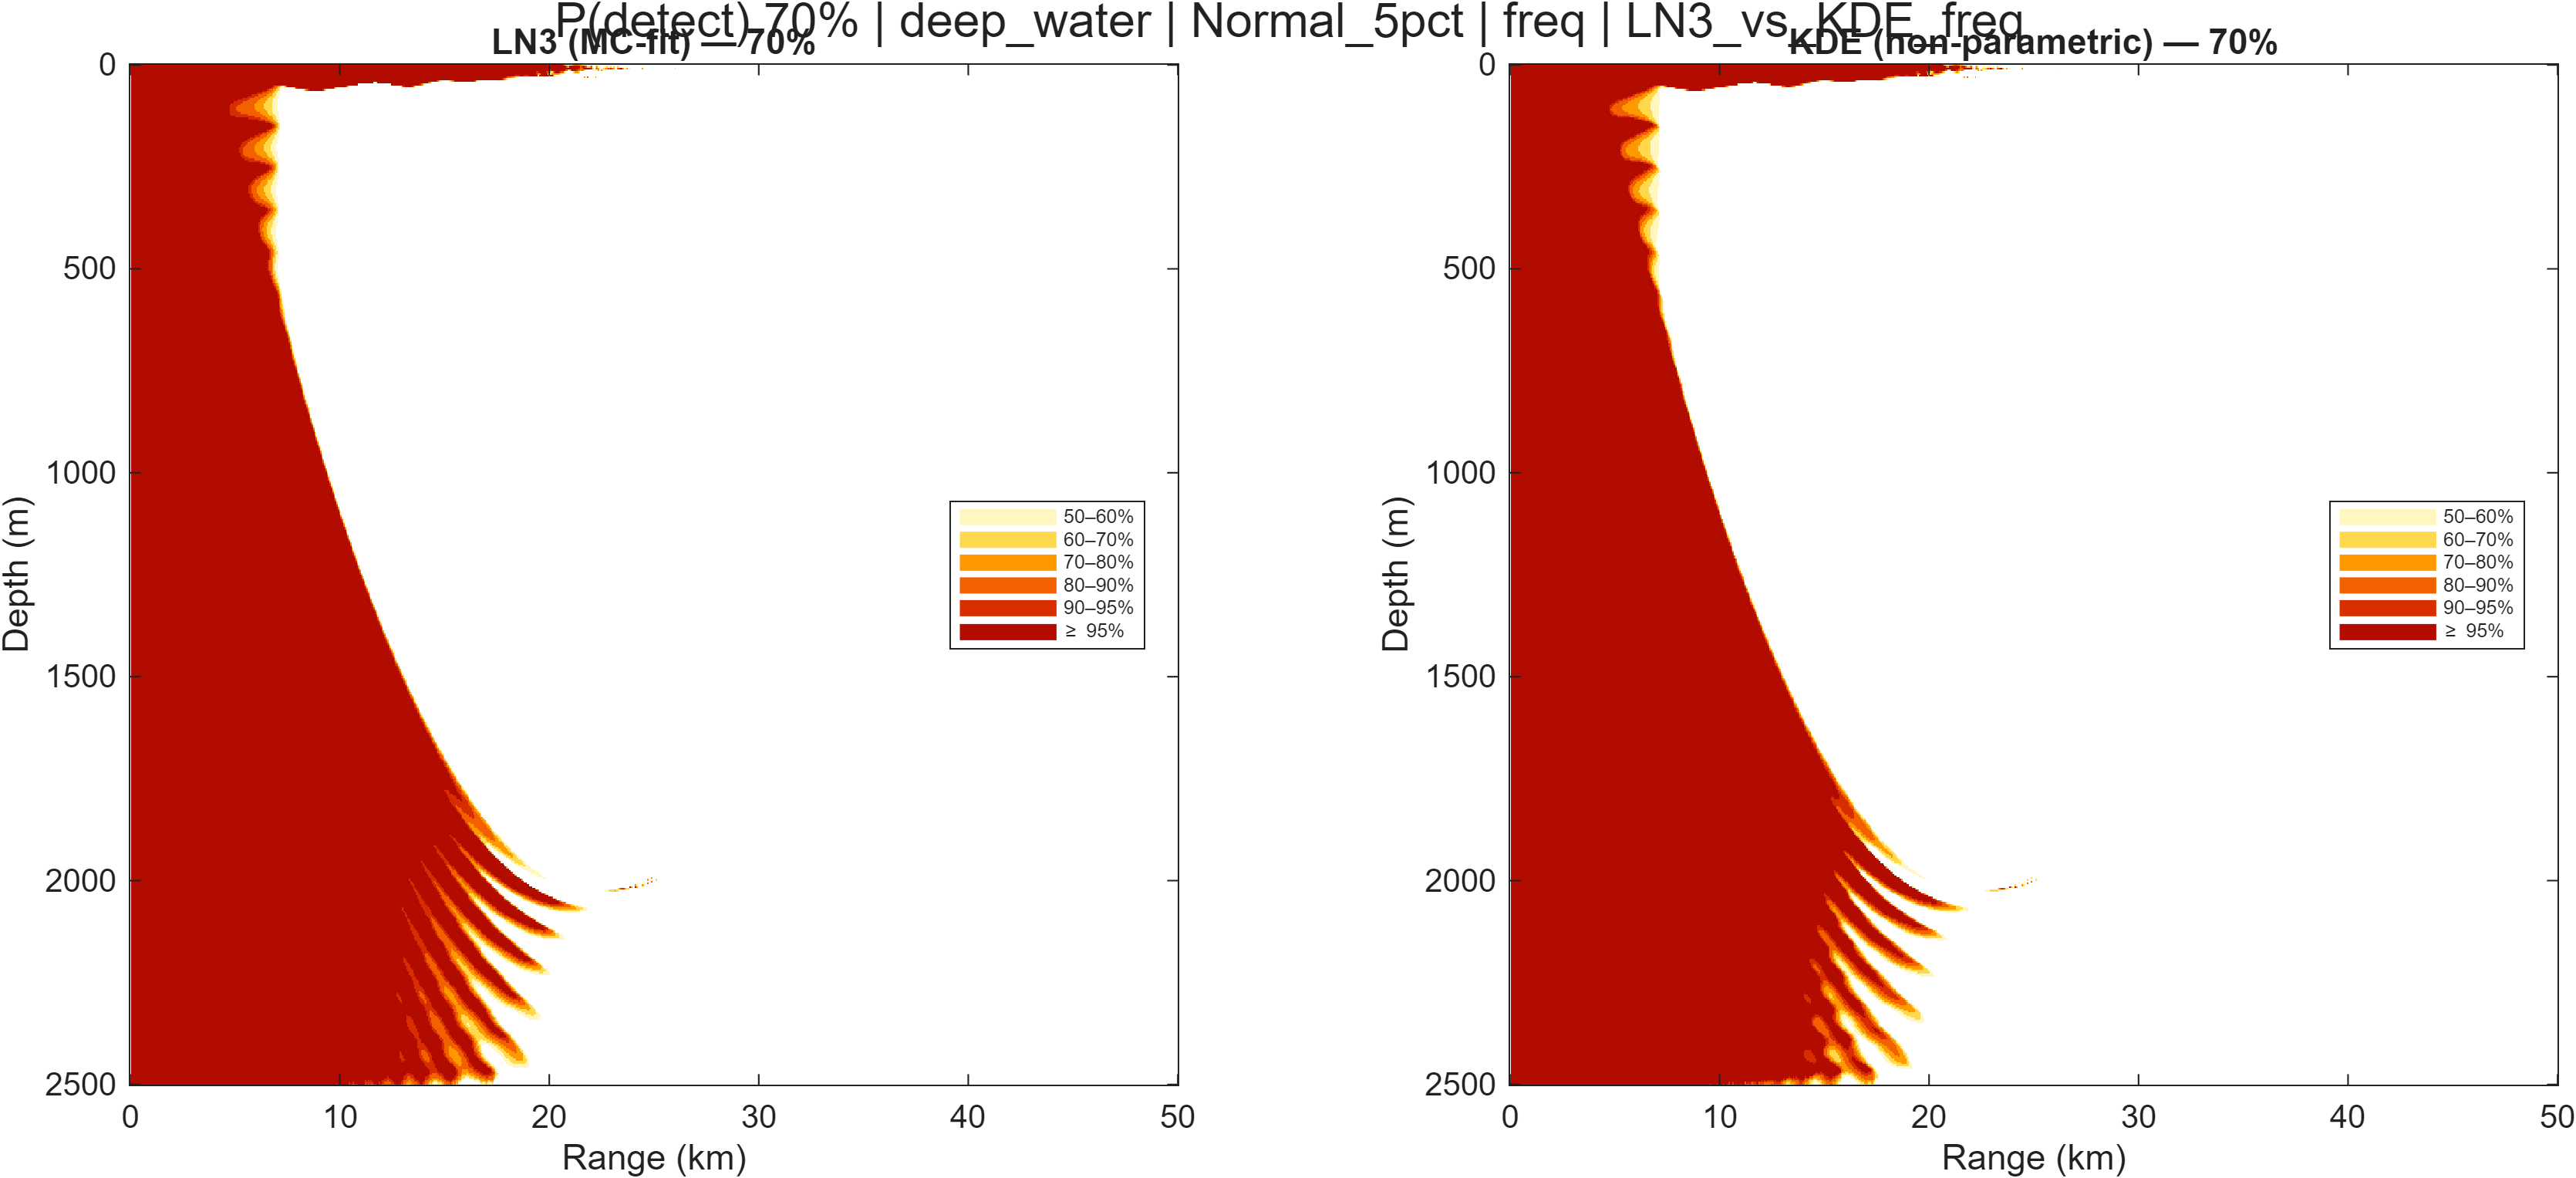
\includegraphics[width=\linewidth]{deep_water/Normal_5pct/figures/shadow_70_LN3_vs_KDE_freq.png}
    \caption{\textbf{LN3 vs.\ KDE הסתברות צל} (הפרעת תדר).
             KDE עוקב מקרוב יותר אחרי ה-MC האמפירי בגבולות CZ
             שבהם LN3 מזלזל בתרומת הזנב הדו-מודלי.}
  \end{subfigure}
  \caption{התכנסות PCE והשוואת מפות גילוי למים עמוקים / נורמלי 5\%{}.}
  \label{fig:gallery_pce_kde}
\end{figure}

% ─────────────────────────────────────────
\subsection{סטטיסטיקת ייחוס מונטה קרלו}
\label{sec:mc}

\begin{english}
Monte Carlo (MC) simulations use \textbf{two complementary sample sets}, each with
$N=1000$ samples per scenario/distribution/parameter combination:
\begin{itemize}
  \item \textbf{LHS set} ($N=1000$ Latin Hypercube samples): provides
        $\hat\EX[\TL]$, $\hat\Var[\TL]$, empirical $\hat P_{\text{det}}$, KDE,
        and the MOM-fitted LN3 reference.
        LHS stratification ensures full coverage of the input space.
  \item \textbf{IID set} ($N=1000$ i.i.d.\ samples): used exclusively for
        MLE-based LN3 fitting, since MLE requires the i.i.d.\ assumption.
\end{itemize}
Both sets are cached at \texttt{Cache/<scenario>/<dist>/} (LHS) and
\texttt{Cache/<scenario>/<dist>\_iid/} (IID), yielding
$4\times3\times3\times2\times1000 = 72\,000$ total Bellhop evaluations.
\end{english}

\begin{figure}[H]
  \centering
  \begin{subfigure}[t]{0.48\textwidth}
    
\includegraphics[width=\linewidth]{shallow_water/Normal_5pct/figures/TL_zS.png}
    \caption{מים רדודים (שטוח, 50~מ')}
  \end{subfigure}\hfill
  \begin{subfigure}[t]{0.48\textwidth}
    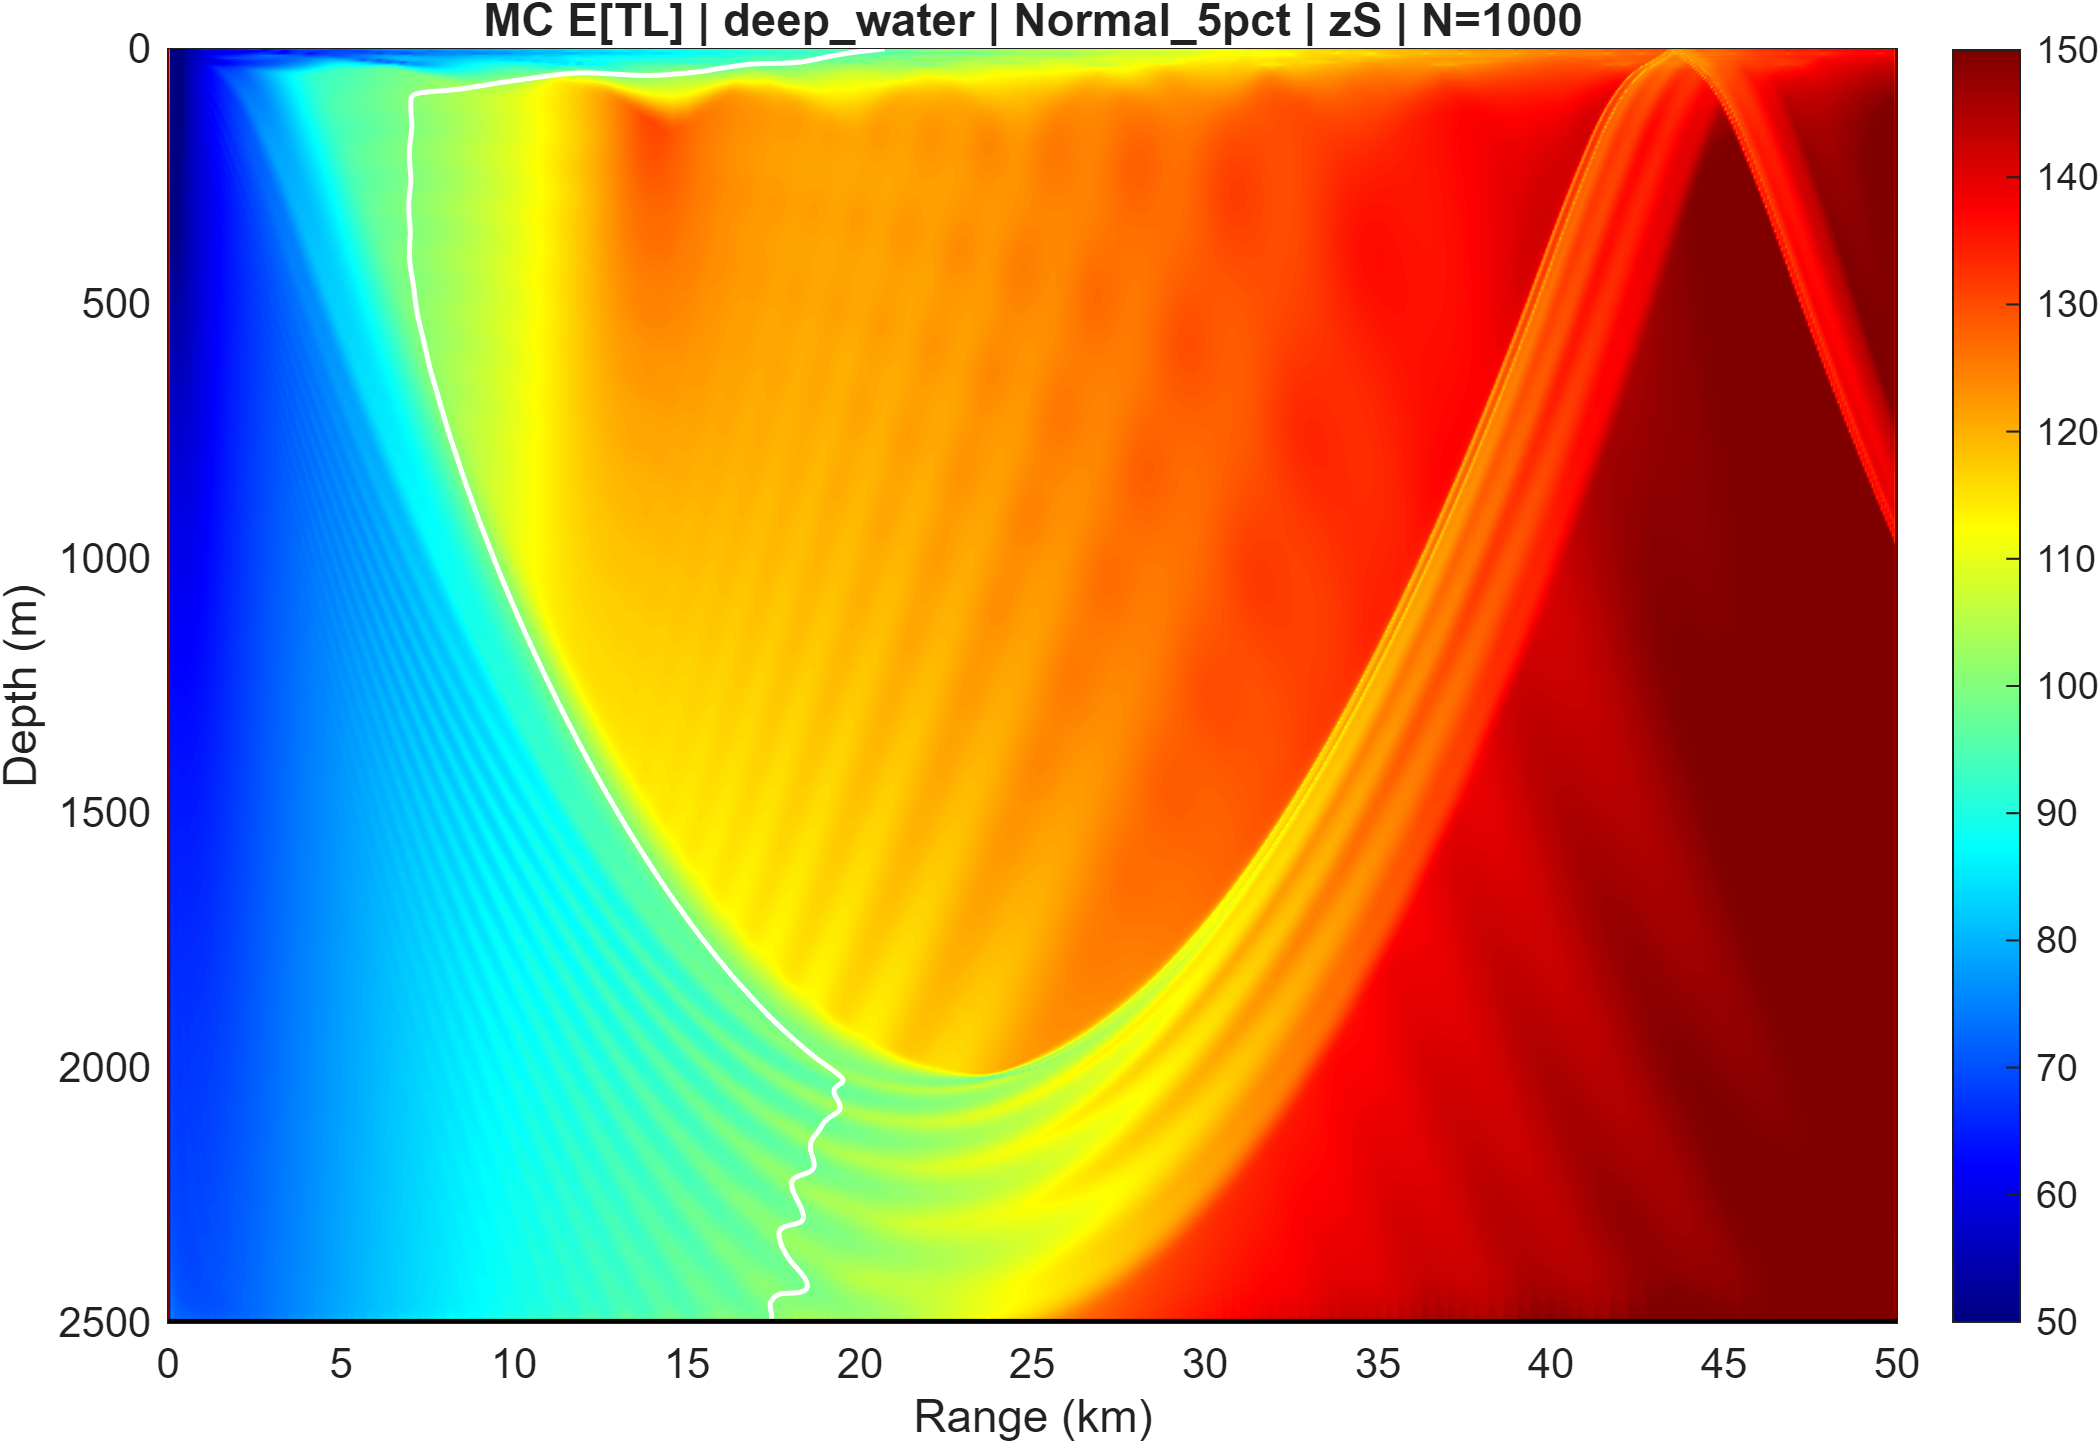
\includegraphics[width=\linewidth]{deep_water/Normal_5pct/figures/TL_zS.png}
    \caption{מים עמוקים (שטוח, 2500~מ')}
  \end{subfigure}\\[8pt]
  \begin{subfigure}[t]{0.48\textwidth}
    
\includegraphics[width=\linewidth]{downslope/Normal_5pct/figures/TL_zS.png}
    \caption{מדרון יורד (50→550~מ'): אזור הצל ממיפוי קרקע בטווח בינוני.}
  \end{subfigure}\hfill
  \begin{subfigure}[t]{0.48\textwidth}
    
\includegraphics[width=\linewidth]{upslope/Normal_5pct/figures/TL_zS.png}
    \caption{מדרון עולה (550→50~מ'): קרקעית עולה לוכדת אנרגיה.}
  \end{subfigure}
  \caption{ממוצע TL של MC $\EX[\TL]$ (dB) להפרעת $z_S$ נורמלי 5\%{} בארבעת התרחישים.}
  \label{fig:mc_ex_var}
\end{figure}

\subsubsection{פרופילי SVP שנדגמו ומודל ההפרעה}
\label{sec:svp_ensemble}

\begin{english}
\paragraph{Physical motivation for the SVP perturbation model.}
The ocean sound-speed profile is not uniform in depth, and its uncertainty is not
uniform either.
The near-surface mixed layer (0--100\,m in summer) is actively stirred by wind and
solar heating; it is nearly isothermal within the mixing depth but its temperature
varies significantly with season and weather.
Below the thermocline, water temperature falls to $\approx 1$--$4\,^\circ$C and
remains essentially constant year-round.
This asymmetry justifies the one-dimensional SVP perturbation model: a scalar shift
$\Delta c$ applied only to the surface mixed layer, coupled to a mixed-layer depth
perturbation $\Delta\mathrm{MLD} = k_{\mathrm{MLD}}\,\Delta c$
($k_{\mathrm{MLD}} = 5\,$m\,s/m, $\mathrm{MLD}_0 = 30\,$m).
The deep SVP gradient ($z > 180\,$m) is held constant because deep-water temperature
variability is an order of magnitude smaller than mixed-layer variability on seasonal
time scales.
\end{english}

\begin{figure}[H]
  \centering
  \begin{subfigure}[t]{0.48\textwidth}
    
\includegraphics[width=\linewidth]{deep_water/Normal_5pct/figures/svp_ensemble.png}
    \caption{נורמלי 5\%{}: $\sigma_{\Delta T}=0.15\,^\circ$C, $\sigma_\mathrm{MLD}=0.75$~מ'.
             ההפרעה מוגבלת לשכבה השטחית מעל $\sim$180~מ'.}
  \end{subfigure}\hfill
  \begin{subfigure}[t]{0.48\textwidth}
    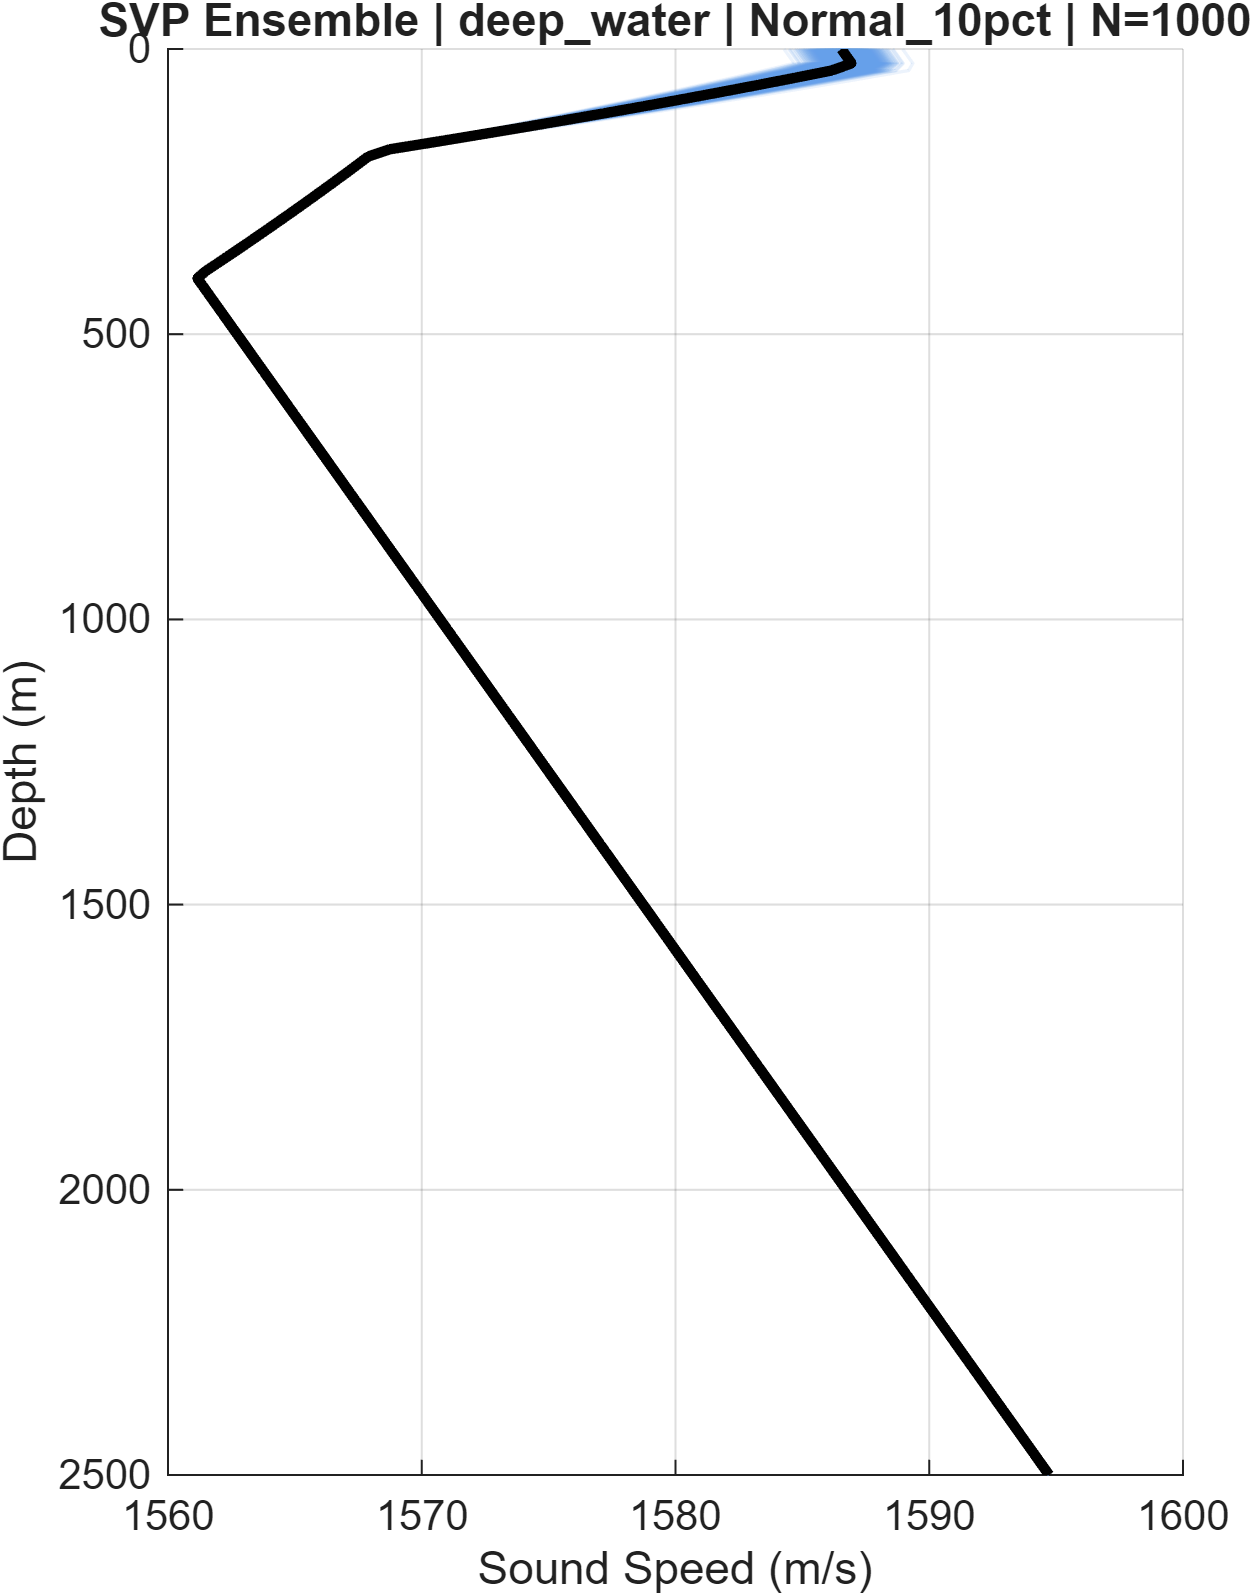
\includegraphics[width=\linewidth]{deep_water/Normal_10pct/figures/svp_ensemble.png}
    \caption{נורמלי 10\%{}: $\sigma_{\Delta T}=0.30\,^\circ$C, $\sigma_\mathrm{MLD}=1.5$~מ'.
             רצועה כחולה רחבה יותר ליד המשטח; פרופיל עמוק לא משתנה.}
  \end{subfigure}
  \caption{אנסמבל SVP ($N=1000$) לתרחיש מים עמוקים.
           עקבות כחולות: פרופילים שנדגמו ב-MC; שחור עבה: פרופיל נומינלי.}
  \label{fig:svp_ensemble}
\end{figure}

\subsubsection{התכנסות מאמד MC}
\label{sec:mc_conv}

\begin{english}
For a scalar random variable $Y$ with finite variance, the sample mean
$\bar Y_N$ converges to $\mu_Y$ at the classical CLT rate
$\mathrm{RMSE}(\bar Y_N) = \sigma_Y / \sqrt{N}$.
The sample variance $S_N^2$ converges at the same asymptotic rate but with a
larger prefactor:
\end{english}
\begin{equation}
  \mathrm{Var}(S_N^2) \;=\; \frac{2\sigma_Y^4}{N-1},
  \label{eq:var_of_var}
\end{equation}
\begin{english}
so the relative error of $S_N^2$ is $\sqrt{2/(N-1)}/C_V^2$ where
$C_V=\sigma_Y/\mu_Y$ is the coefficient of variation.
At $N=1000$ and for the broadest distribution (Normal\,10\%), the relative RMSE
of the sample variance estimator is $\approx 4.5\%$, within the $\lesssim 5\%$
target.
\end{english}

\begin{figure}[H]
  \centering
  \begin{subfigure}[t]{0.48\textwidth}
    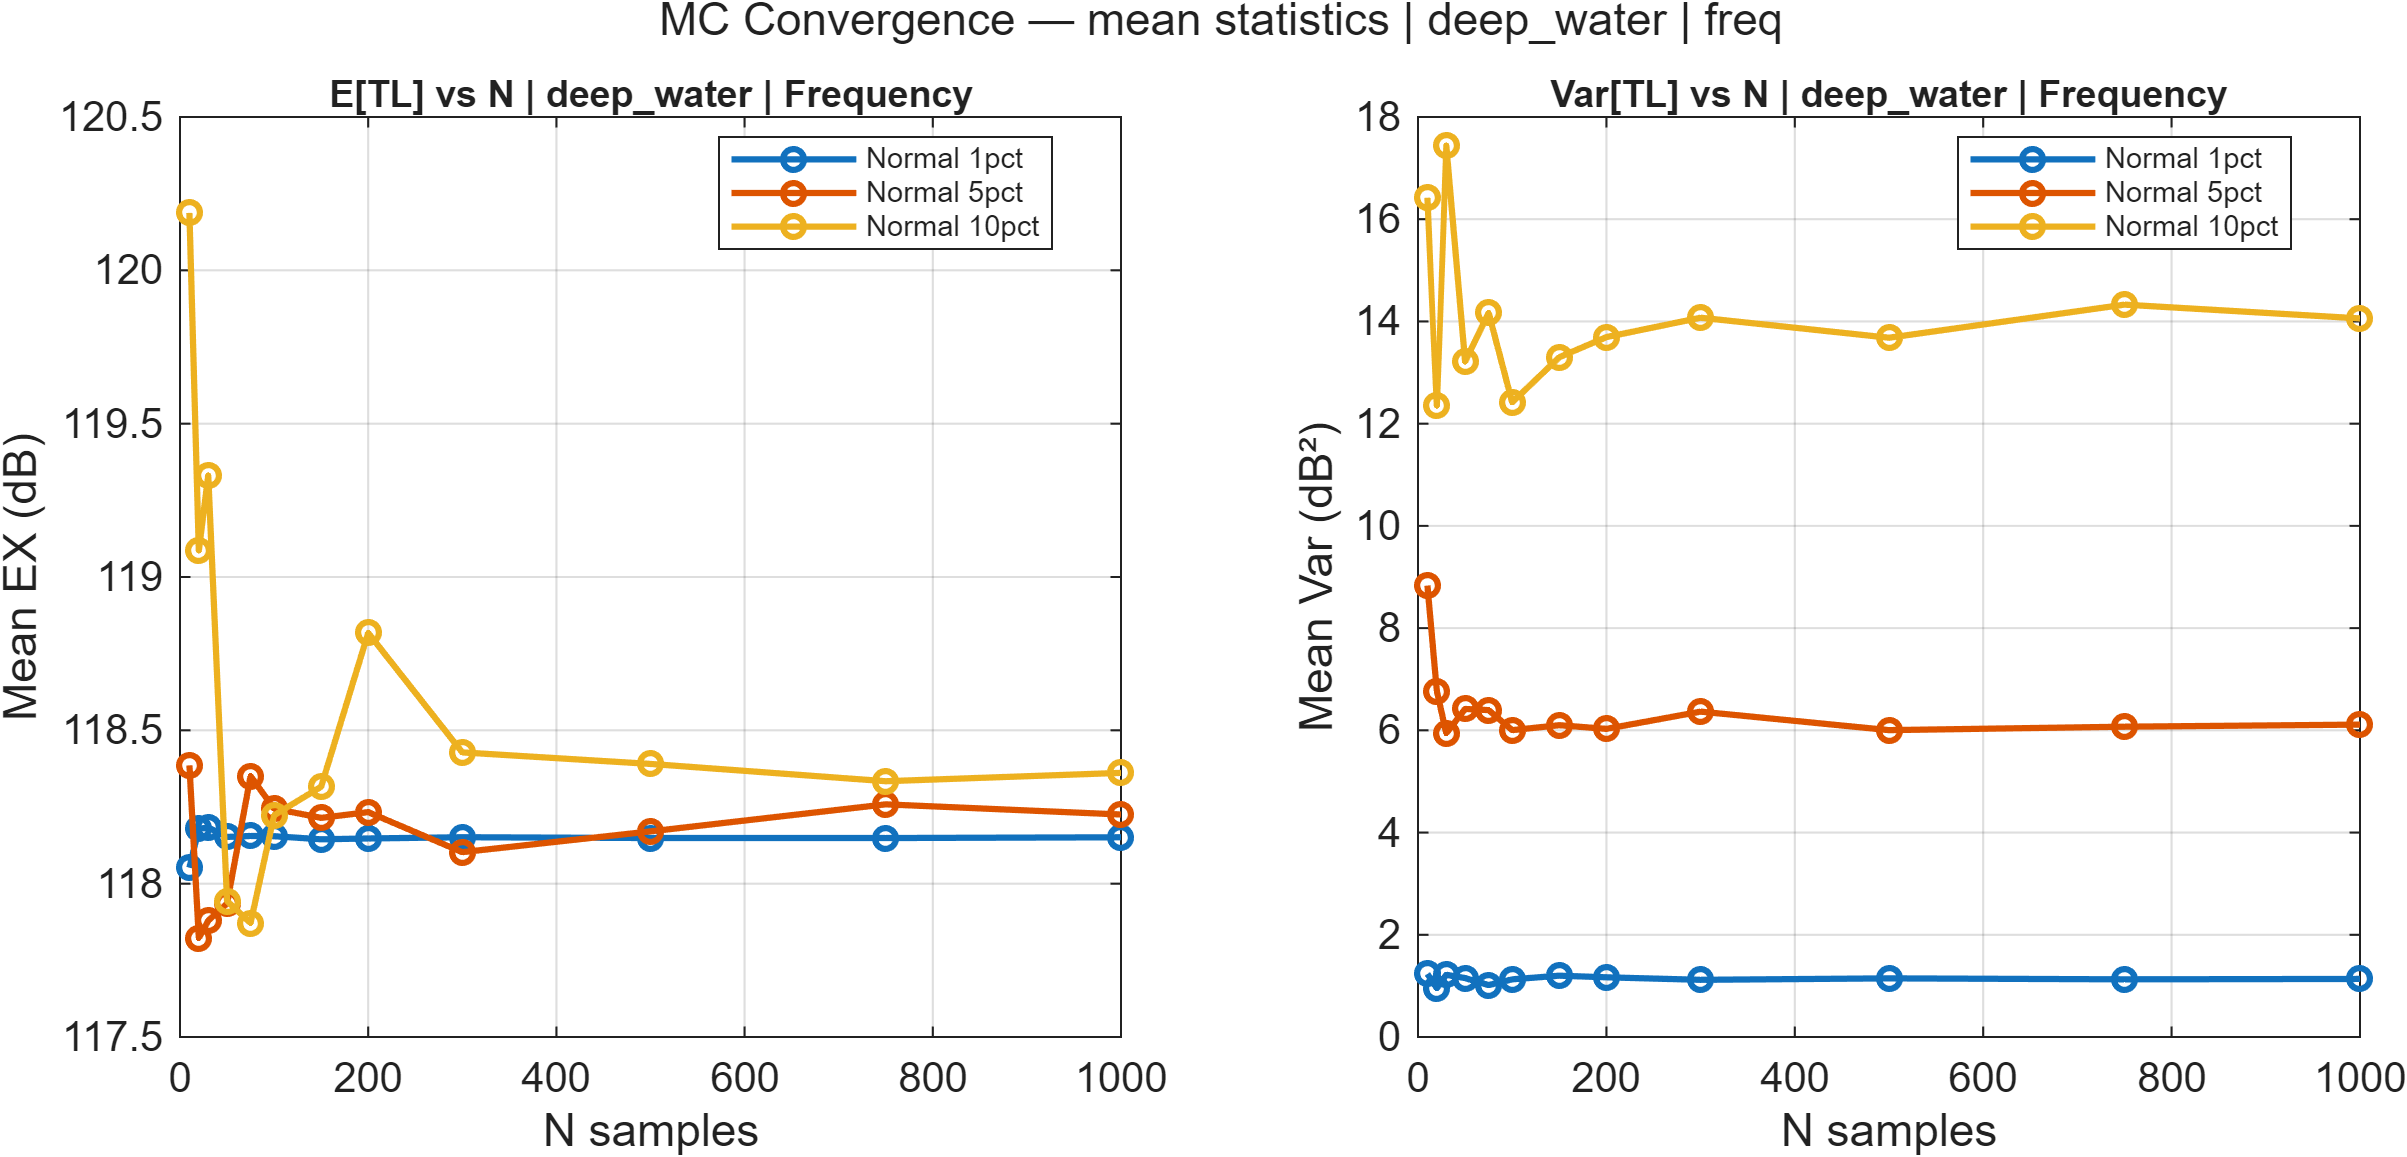
\includegraphics[width=\linewidth]{deep_water/figures/mc_conv_mean_freq.png}
    \caption{תדר: $\hat\EX[\TL]$ ו-$\hat\Var[\TL]$ מול $N$.}
  \end{subfigure}\hfill
  \begin{subfigure}[t]{0.48\textwidth}
    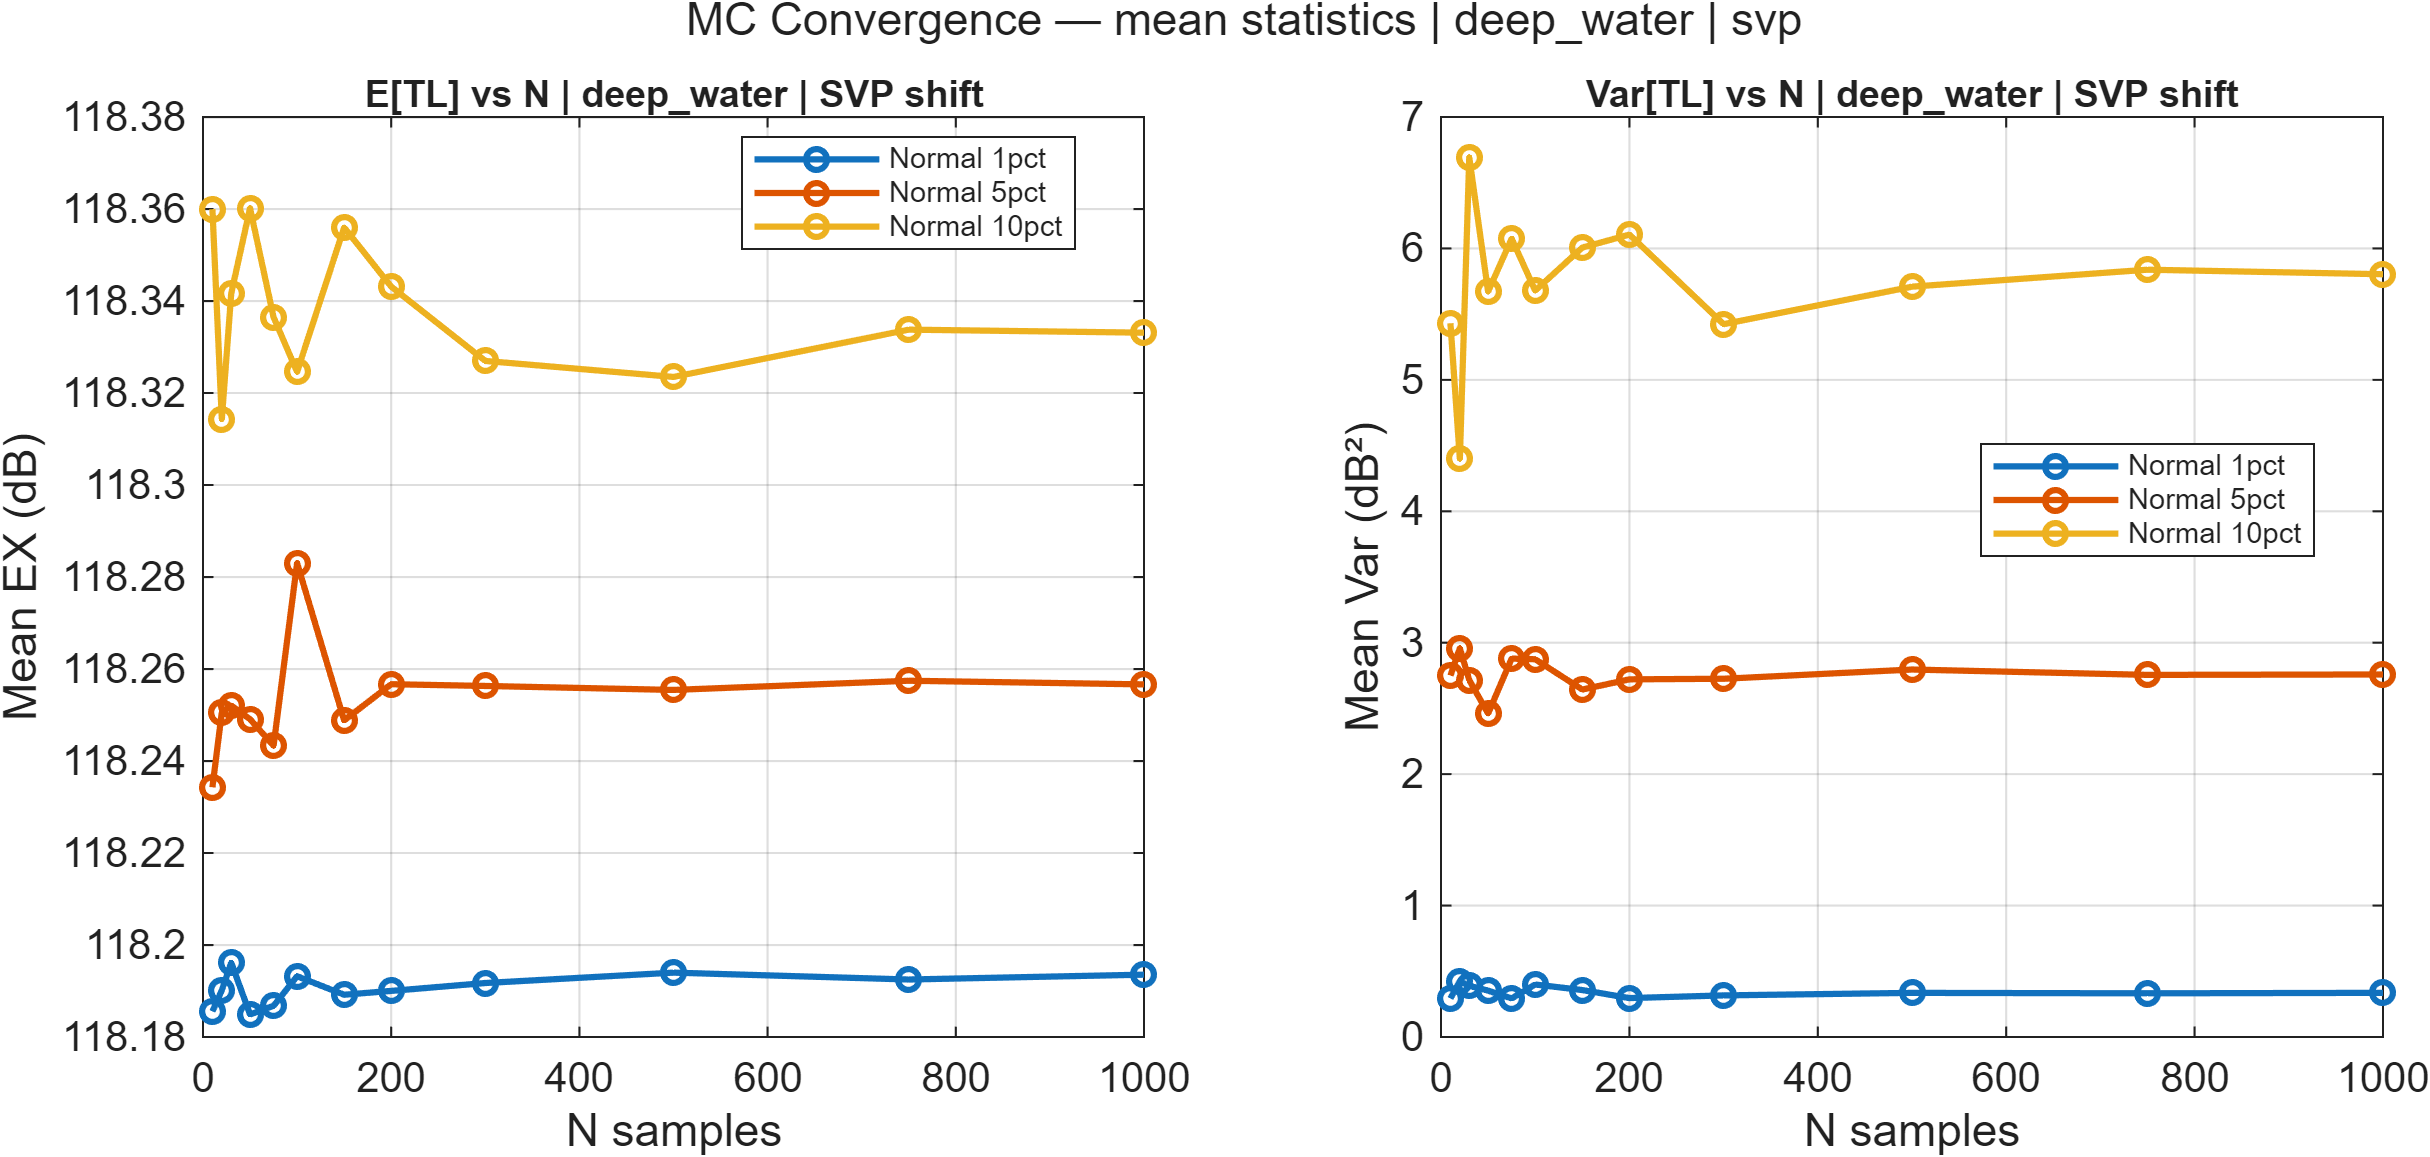
\includegraphics[width=\linewidth]{deep_water/figures/mc_conv_mean_svp.png}
    \caption{SVP: $\hat\EX[\TL]$ ו-$\hat\Var[\TL]$ מול $N$.}
  \end{subfigure}
  \caption{התכנסות מאמד MC לתרחיש מים עמוקים ($N=10$ עד $1000$).
           ממוצע מתכנס מהר יותר משונות, בהתאם למשוואה~\ref{eq:var_of_var}.}
  \label{fig:mc_conv}
\end{figure}

% ─────────────────────────────────────────
\subsection{שיטת דלתא מסדר ראשון: דיוק ומצבי כשל}
\label{sec:delta}

\begin{english}
\paragraph{Terminology note.}
The term \emph{Delta method} here refers to linearisation via perturbation calculus
(first-order Taylor expansion of the model output around the nominal parameter vector),
also known as FOSM (First-Order Second-Moment method) in structural reliability
and as GUM linearisation in metrology.

The 1st-order Delta method approximates variance as:
\end{english}
\begin{equation}
  \Var_1[\TL] \;\approx\; \sum_{i} J_i^2 \,\sigma_i^2,
  \qquad J_i = \frac{\partial \TL}{\partial \theta_i}\bigg|_{\boldsymbol{\theta}_0},
  \label{eq:delta1}
\end{equation}
\begin{english}
where Jacobians $J_i$ are computed via central finite differences.
The 2nd-order extension adds Hessian correction terms
$\tfrac{1}{2} H_{ii}^2 \kappa_i$ where $\kappa_i = \EX[\delta\theta_i^4]/\sigma_i^4 - 1$
is the excess kurtosis.
\end{english}

\subsubsection{היכן שיטת דלתא מצליחה}

\begin{english}
For the \textbf{shallow-water} and \textbf{deep-water} scenarios under small
perturbations ($\leq$1\% uncertainty), the Delta method achieves relative $L_1$
errors below 10\% in the variance maps.
The shadow-probability maps computed via the Delta--LN3 hybrid agree closely with
empirical MC shadow probabilities in these scenarios.
\end{english}

\begin{figure}[H]
  \centering
  \begin{subfigure}[t]{0.48\textwidth}
    
\includegraphics[width=\linewidth]{shallow_water/Normal_1pct/figures/shadow_70_MC_vs_Delta_zS.png}
    \caption{MC vs.\ Delta}
  \end{subfigure}\hfill
  \begin{subfigure}[t]{0.48\textwidth}
    
\includegraphics[width=\linewidth]{shallow_water/Normal_1pct/figures/shadow_70_MC_vs_DeltaLN3_zS.png}
    \caption{MC vs.\ Delta--LN3}
  \end{subfigure}\\[8pt]
  \begin{subfigure}[t]{0.48\textwidth}
    
\includegraphics[width=\linewidth]{shallow_water/Normal_1pct/figures/shadow_70_MC_vs_LN3_zS.png}
    \caption{MC vs.\ LN3}
  \end{subfigure}
  \caption{השוואת Delta vs.\ MC vs.\ Delta--LN3 הסתברות צל ($P(\TL > 70$~dB$)$)
           שבה השיטות האנליטיות \emph{מסכימות} עם MC
           (מים רדודים, נורמלי 1\%{}, הפרעת $z_S$).
           בכל פאנל: MC אמפירי — חצי שמאל; קירוב אנליטי — חצי ימין.}
  \label{fig:shadow_good}
\end{figure}

\subsubsection{היכן שיטת דלתא נכשלת}

\begin{english}
For \textbf{slope scenarios} (upslope, downslope) and large perturbations
($\geq$5\%), the 1st-order approximation breaks down significantly.
The 2nd-order correction is equally unable to recover the variance:
the Hessian correction term $|\kappa H^2|/V_1$ exceeds 100\% for SVP perturbations
in both slope scenarios, indicating that the Taylor series has not converged at
2nd order.
\end{english}

\begin{figure}[H]
  \centering
  \begin{subfigure}[t]{0.48\textwidth}
    
\includegraphics[width=\linewidth]{downslope/Normal_5pct/figures/shadow_70_MC_vs_Delta_svp.png}
    \caption{MC vs.\ Delta}
  \end{subfigure}\hfill
  \begin{subfigure}[t]{0.48\textwidth}
    
\includegraphics[width=\linewidth]{downslope/Normal_5pct/figures/shadow_70_MC_vs_DeltaLN3_svp.png}
    \caption{MC vs.\ Delta--LN3}
  \end{subfigure}\\[8pt]
  \begin{subfigure}[t]{0.48\textwidth}
    
\includegraphics[width=\linewidth]{downslope/Normal_5pct/figures/shadow_70_MC_vs_LN3_svp.png}
    \caption{MC vs.\ LN3}
  \end{subfigure}
  \caption{השוואת הסתברות צל שבה Delta מסדר 1 \emph{נכשל}
           (מדרון יורד, נורמלי 5\%{}, הפרעת SVP).
           אי-הסכמה בולטת בגבול אזור ההצל מאשרת כי סדרת טיילור לא התכנסה.}
  \label{fig:shadow_bad}
\end{figure}

\begin{table}[H]
  \centering
  \caption{תיקון ממוצע מסדר 2:
           $\langle|\kappa H^2|/(J^2\sigma^2 + |\kappa H^2|)\rangle$ [\%].
           ערכים $>$50\%{} מצביעים על כך שהקירוב מסדר 1 אינו מספיק.}
  \label{tab:2nd_order_correction}
  \begin{english}
  \begin{tabular}{lcccccc}
    \toprule
    & \multicolumn{2}{c}{Normal 5\%} & \multicolumn{2}{c}{Normal 10\%}
    & \multicolumn{2}{c}{Normal 10\%} \\
    \cmidrule(lr){2-3}\cmidrule(lr){4-5}\cmidrule(lr){6-7}
    Scenario & Total & SVP & Total & SVP & Total & SVP \\
    \midrule
    Shallow water & 96.6 & 98.2 & 99.1 & 99.5 & 99.5 & 99.8 \\
    Deep water    & 97.0 & 51.7 & 99.2 & 81.1 & 99.6 & 88.9 \\
    Upslope       & 97.5 & 73.0 & 99.4 & 91.5 & 99.7 & 95.3 \\
    Downslope     & 96.1 & 81.1 & 99.0 & 94.5 & 99.5 & 97.0 \\
    \bottomrule
  \end{tabular}
  \end{english}
\end{table}

\subsubsection{סינתזת תוצאות שיטת דלתא}

\begin{english}
The Delta method results reveal a two-factor failure mode governed by
\emph{perturbation magnitude} and \emph{bathymetric complexity}:

\begin{itemize}
  \item \textbf{Small perturbations ($\sigma\leq$1\%), flat bathymetry.}
        The 1st-order Taylor linearisation is valid; shadow-probability maps from
        the Delta--LN3 hybrid agree closely with MC.

  \item \textbf{Moderate-to-large perturbations ($\sigma\geq$5\%), flat bathymetry.}
        The 2nd-order Hessian correction term already exceeds the 1st-order term for
        all scenarios except deep-water SVP at 5\%.
        The Taylor series has \emph{not converged} at order~2 in almost all cases.

  \item \textbf{Slope environments (upslope, downslope), any perturbation.}
        The bathymetric gradient introduces refraction-driven shadow zones whose
        spatial location depends sensitively on the uncertain parameters.
        Even at $\sigma=1\%$, the Delta--LN3 shadow maps exhibit significant spatial
        mismatch relative to MC.
\end{itemize}

\textbf{Practical implication.} The Delta method is only trustworthy for sonar
planning in flat-bottom environments under $\leq$1\% uncertainty in each parameter.
For 5--10\% uncertainty or any slope environment, either PCE or direct MC is required.
\end{english}

% ─────────────────────────────────────────
\subsection{אמידת הסתברות הצל — LN3}
\label{sec:ln3}

\begin{english}
\paragraph{A priori motivation for the LN3 model.}
The choice of a three-parameter lognormal distribution for TL is motivated by
physical arguments:

First, TL is already expressed on a logarithmic (dB) scale:
$\mathrm{TL} = -20\log_{10}(|p|/p_0)$.
Any multiplicative structure in the pressure field therefore maps to an additive
structure in TL, favouring distributions from the lognormal family.

Second, in a multi-mode waveguide the received pressure is a coherent sum of $M$
normal-mode contributions; for large $M$ the CLT suggests that $|p|$ is approximately
Rayleigh-distributed, which converts to approximately lognormal TL.

Third, TL has a physical lower bound: geometric spreading imposes a minimum loss
$\mathrm{TL}_{\min} > 0\,\mathrm{dB}$.
The three-parameter lognormal
\end{english}
\begin{equation}
  X - \gamma \sim \mathrm{LN2}, \quad \gamma = 0.95\,\min(\text{samples}),
\end{equation}
\begin{english}
explicitly encodes this physical floor through the shift parameter $\gamma$.
Parameters $(\hat\mu, \hat\sigma)$ are estimated by MLE via \texttt{lognfit}
(superior to MOM, which is typically 10--30\% less efficient):
\end{english}
\begin{equation}
  \hat{P}_{\mathrm{shadow}}^{\mathrm{LN3}}(\mathbf{x})
  = \Phi\!\left(\frac{\ln(\mathrm{FOM}-\hat\gamma)-\hat\mu}{\hat\sigma}\right).
\end{equation}

\subsubsection{שגיאת RMSE של CDF בשלושה תרחישים}

\begin{figure}[H]
  \centering
  \begin{subfigure}[b]{0.48\textwidth}
    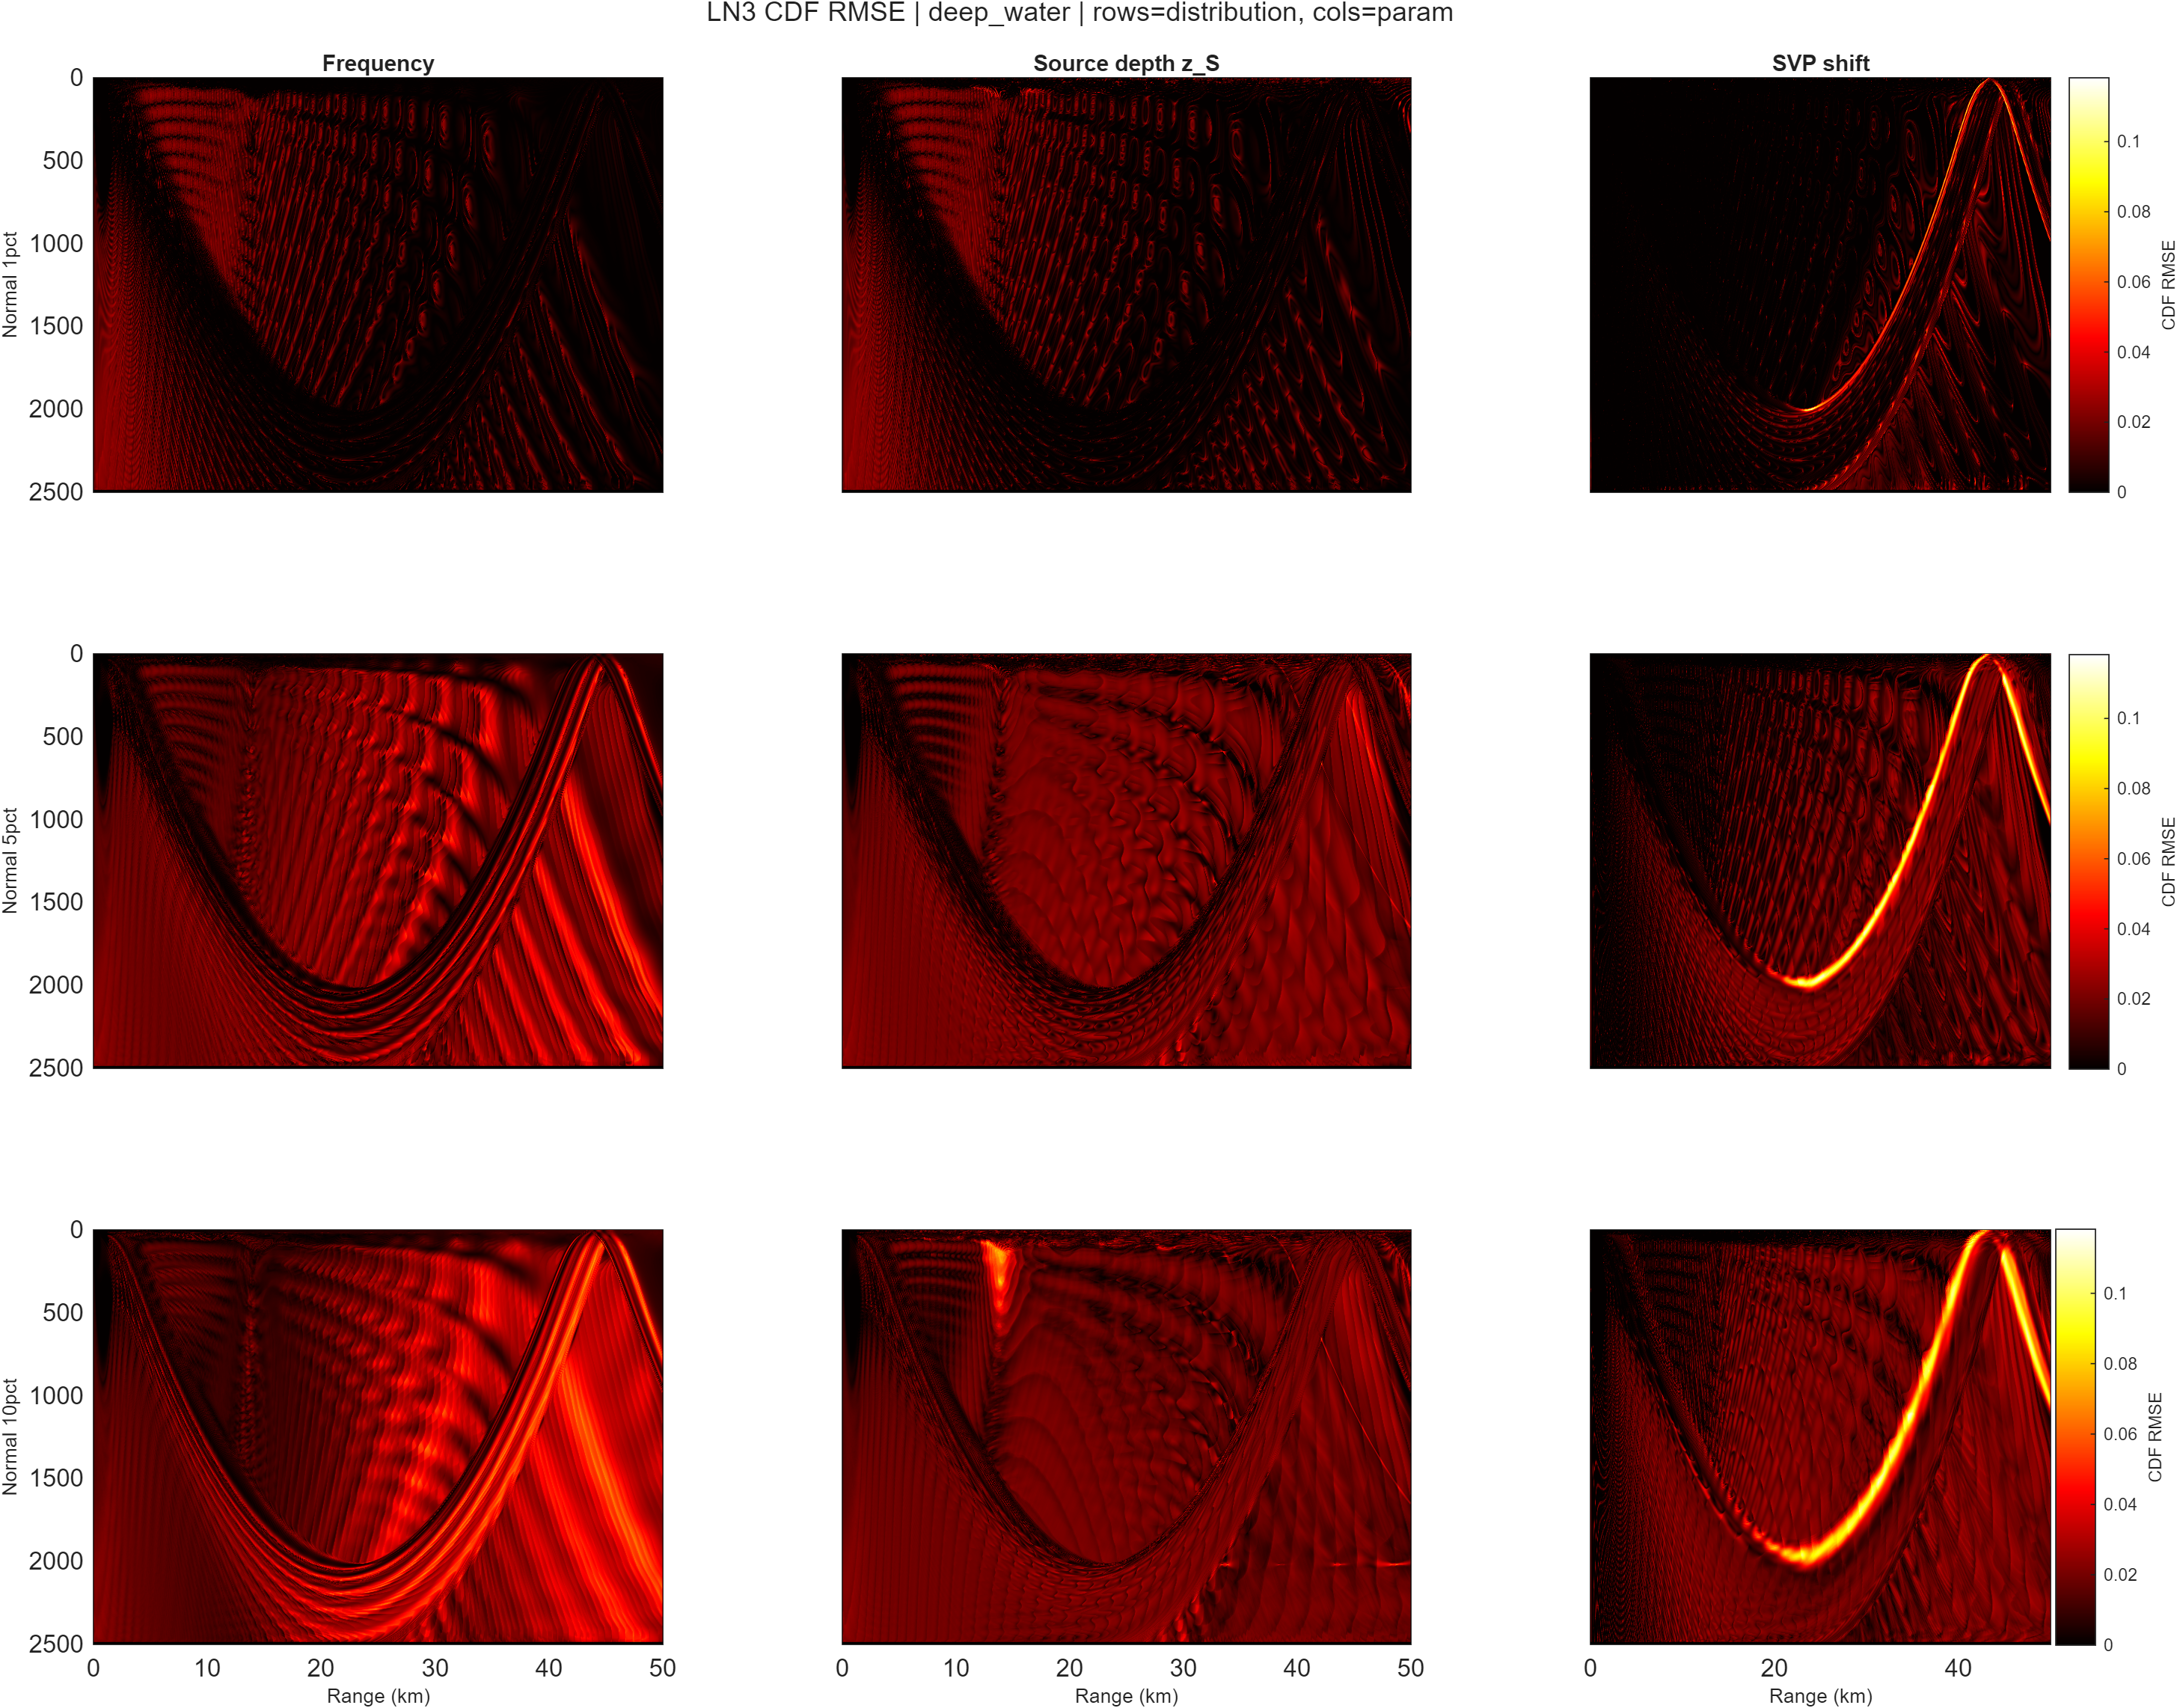
\includegraphics[width=\linewidth]{deep_water/figures/LN3_RMSE_all.png}
    \caption{מים עמוקים}
  \end{subfigure}\hfill
  \begin{subfigure}[b]{0.48\textwidth}
    
\includegraphics[width=\linewidth]{shallow_water/figures/LN3_RMSE_all.png}
    \caption{מים רדודים}
  \end{subfigure}\\[0.4em]
  \begin{subfigure}[b]{0.48\textwidth}
    
\includegraphics[width=\linewidth]{upslope/figures/LN3_RMSE_all.png}
    \caption{מדרון עולה}
  \end{subfigure}\hfill
  \begin{subfigure}[b]{0.48\textwidth}
    
\includegraphics[width=\linewidth]{downslope/figures/LN3_RMSE_all.png}
    \caption{מדרון יורד}
  \end{subfigure}
  \caption{שגיאת RMSE של CDF LN3 (בין LN3 ל-MC) בארבעת התרחישים
           ושלוש רמות האי-ודאות.
           שורות: נורמלי 1\%{}/5\%{}/10\%{}. עמודות: \textenglish{freq, $z_S$, SVP}.
           כהה = התאמה טובה; בהיר = כשל ב-CZ.}
  \label{fig:ln3_rmse}
\end{figure}

\subsubsection{כשל דו-מודלי בגבולות CZ}

\begin{english}
At pixels near convergence-zone boundaries, the TL distribution becomes bimodal:
the acoustic field switches between a focused (low TL) and defocused (high TL) state
as SVP varies, and no unimodal lognormal can capture both modes simultaneously.
\end{english}

\begin{figure}[H]
  \centering
  \includegraphics[width=0.85\textwidth]%
    {deep_water/Normal_5pct/figures/bimodal_histogram_svp.png}
  \caption{היסטוגרמה דו-מודלית של TL בפיקסל בעל השונות המרבית
           (מים עמוקים 5\%{}, SVP).
           כחול: מדגמי MC; כתום: LN3 המותאם; קו אדום: רמת FOM.
           LN3 חד-שיאי לא מצליח לתאר את שני השיאים.}
  \label{fig:bimodal}
\end{figure}

\begin{english}
\textbf{Practical note.} In bimodal regimes (CZ, shadow boundaries) neither MLE nor
MOM resolves the fit failure; a mixture-of-lognormals model would be required
regardless of estimator.
The shift parameter $\gamma = 0.95\min(\mathrm{samples})$ remains a heuristic ---
full 3-parameter MLE would require nonlinear optimisation per pixel (computationally
prohibitive at $\sim$440\,000 pixels $\times$ 12 combos).
\end{english}

\subsubsection{MLE מול MOM — השוואת גרזן}

\begin{english}
MLE fits have been compared against MOM estimates across all scenarios.
MLE is systematically more efficient: lower bias and 10--30\% lower RMSE in both
$\hat\mu$ and $\hat\sigma$ estimates. The MOM estimates are used only as a
cross-check.
\end{english}

\begin{figure}[H]
  \centering
  \IfFileExists{deep_water/Normal_5pct/figures/LN3_MOM_vs_MLE_scatter_freq.png}{%
    \includegraphics[width=0.7\textwidth]%
      {deep_water/Normal_5pct/figures/LN3_MOM_vs_MLE_scatter_freq.png}%
  }{\fbox{\parbox[c][3cm][c]{0.7\textwidth}{\centering\small
    LN3 MOM vs MLE scatter — טרם נוצר}}}
  \caption{פיזור MOM מול MLE לפרמטר $\hat\mu$ (מים עמוקים, 5\%{}, תדר).
           מדגים כי MLE עקבי ויעיל יותר.}
  \label{fig:ln3_mom_mle}
\end{figure}

% ─────────────────────────────────────────
\subsection{אימות KDE של הסתברות גילוי}
\label{sec:kde_validation}

\begin{english}
Kernel Density Estimation (KDE) provides a non-parametric approximation of the TL
CDF at each pixel using the Parzen--Rosenblatt window:
\end{english}
\begin{equation}
  \hat{P}_{\mathrm{shadow}}^{\mathrm{KDE}}(\mathbf{x})
  = \frac{1}{N}\sum_{i=1}^N \Phi\!\left(\frac{\mathrm{FOM}-\TL^{(i)}(\mathbf{x})}{h}\right),
\end{equation}
\begin{english}
where the bandwidth $h$ is set by Silverman's rule: $h = 1.06\,\hat\sigma_{\TL}\,N^{-1/5}$.
The three-column KDE validation figures show: (i) MC empirical $\Pshadow$,
(ii) KDE estimate, and (iii) pixel-wise difference map.
\end{english}

\begin{figure}[H]
  \centering
  \begin{subfigure}[b]{0.32\textwidth}
    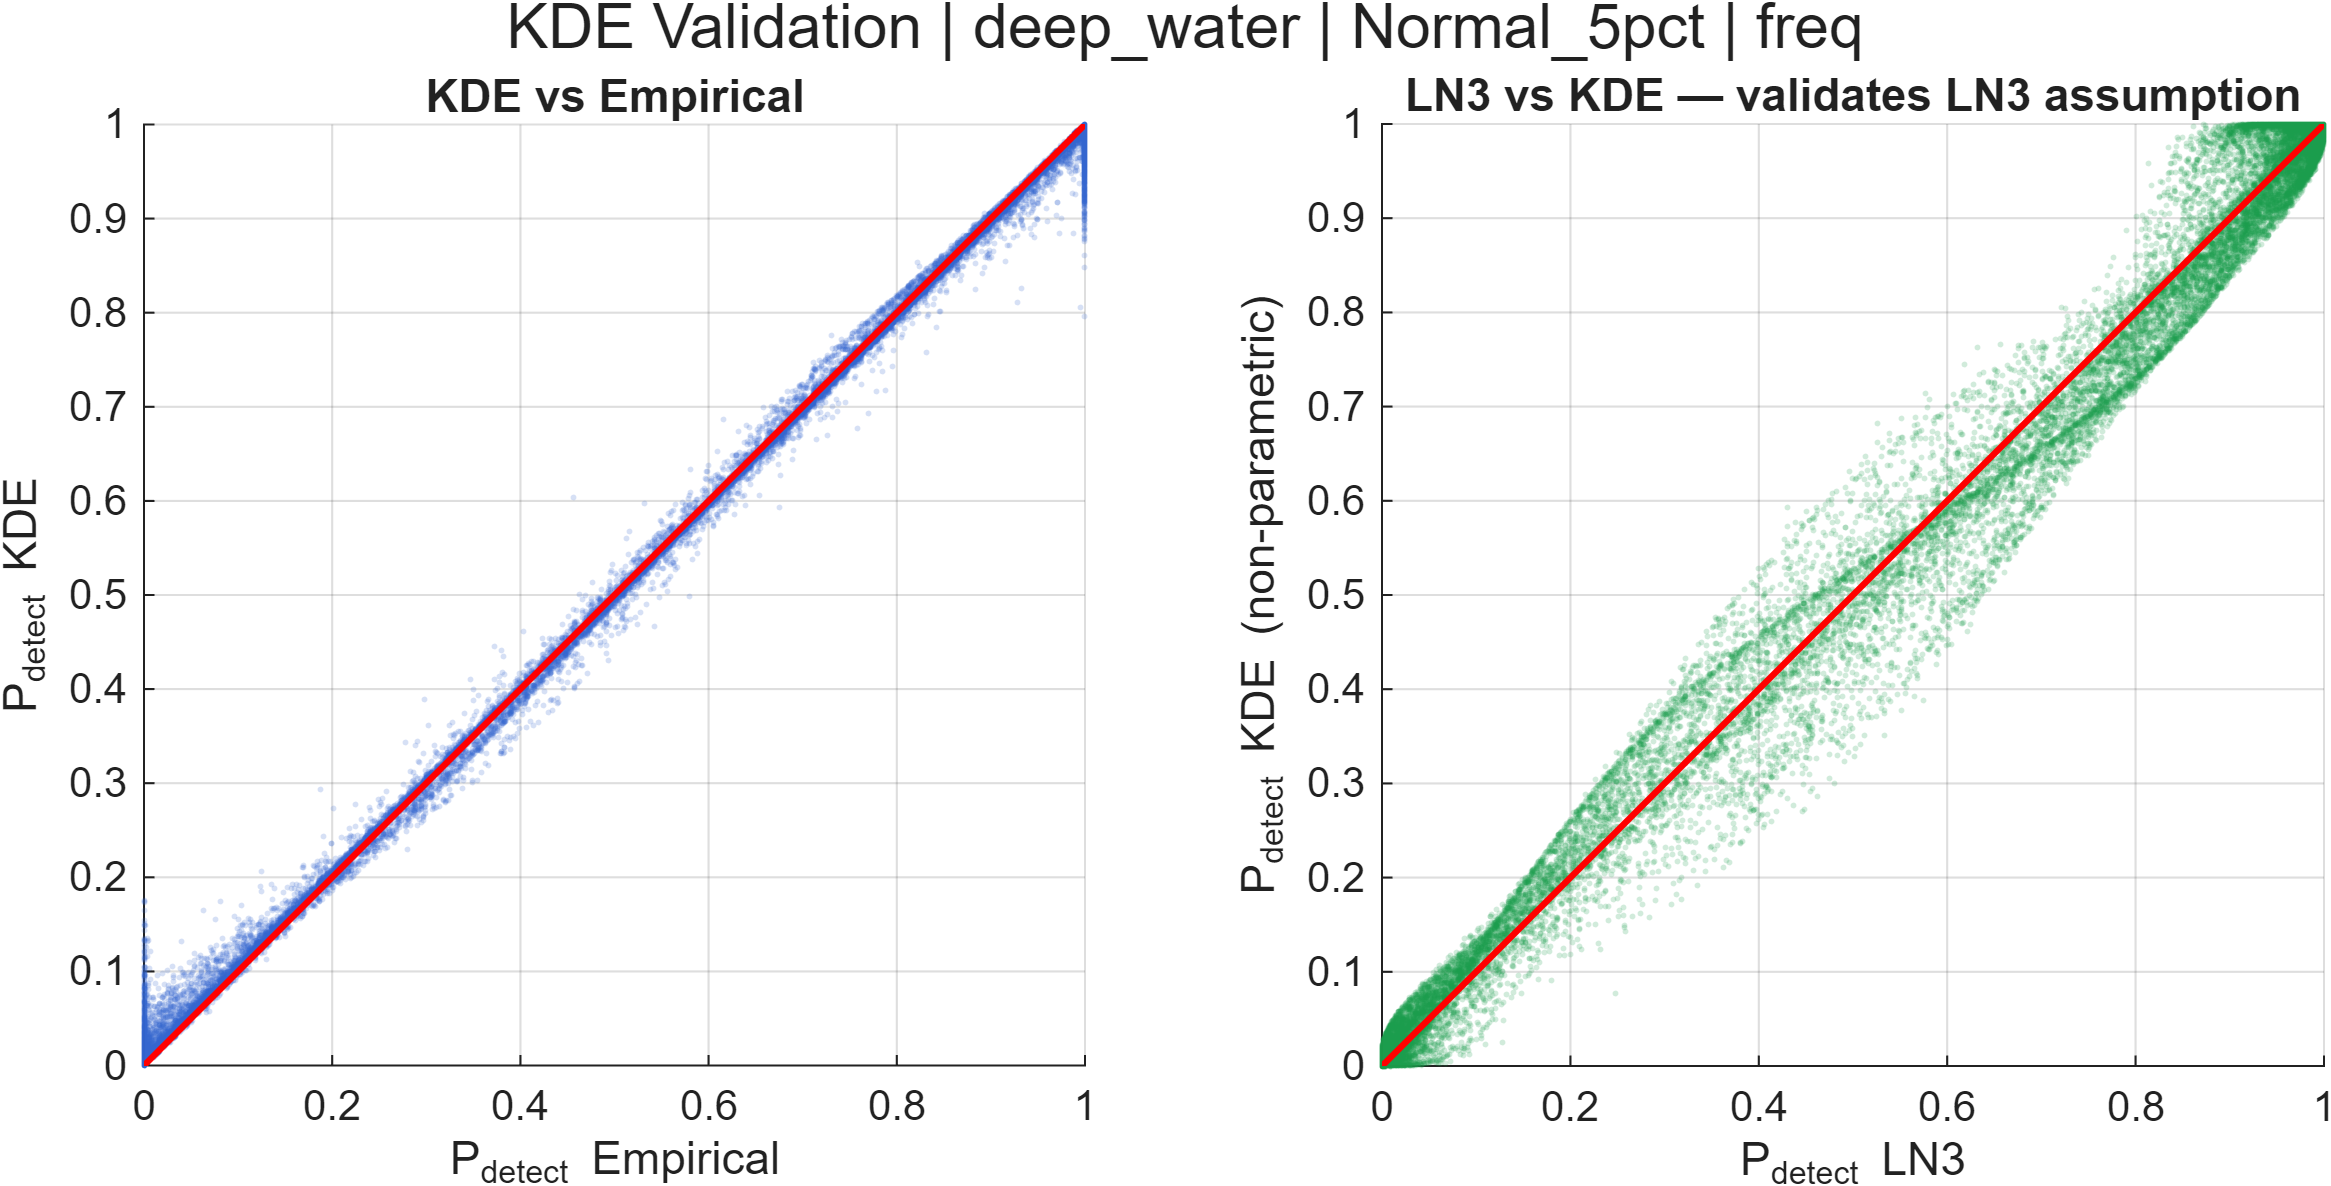
\includegraphics[width=\linewidth]{deep_water/Normal_5pct/figures/kde_validation_freq.png}
    \caption{תדר — מים עמוקים}
  \end{subfigure}\hfill
  \begin{subfigure}[b]{0.32\textwidth}
    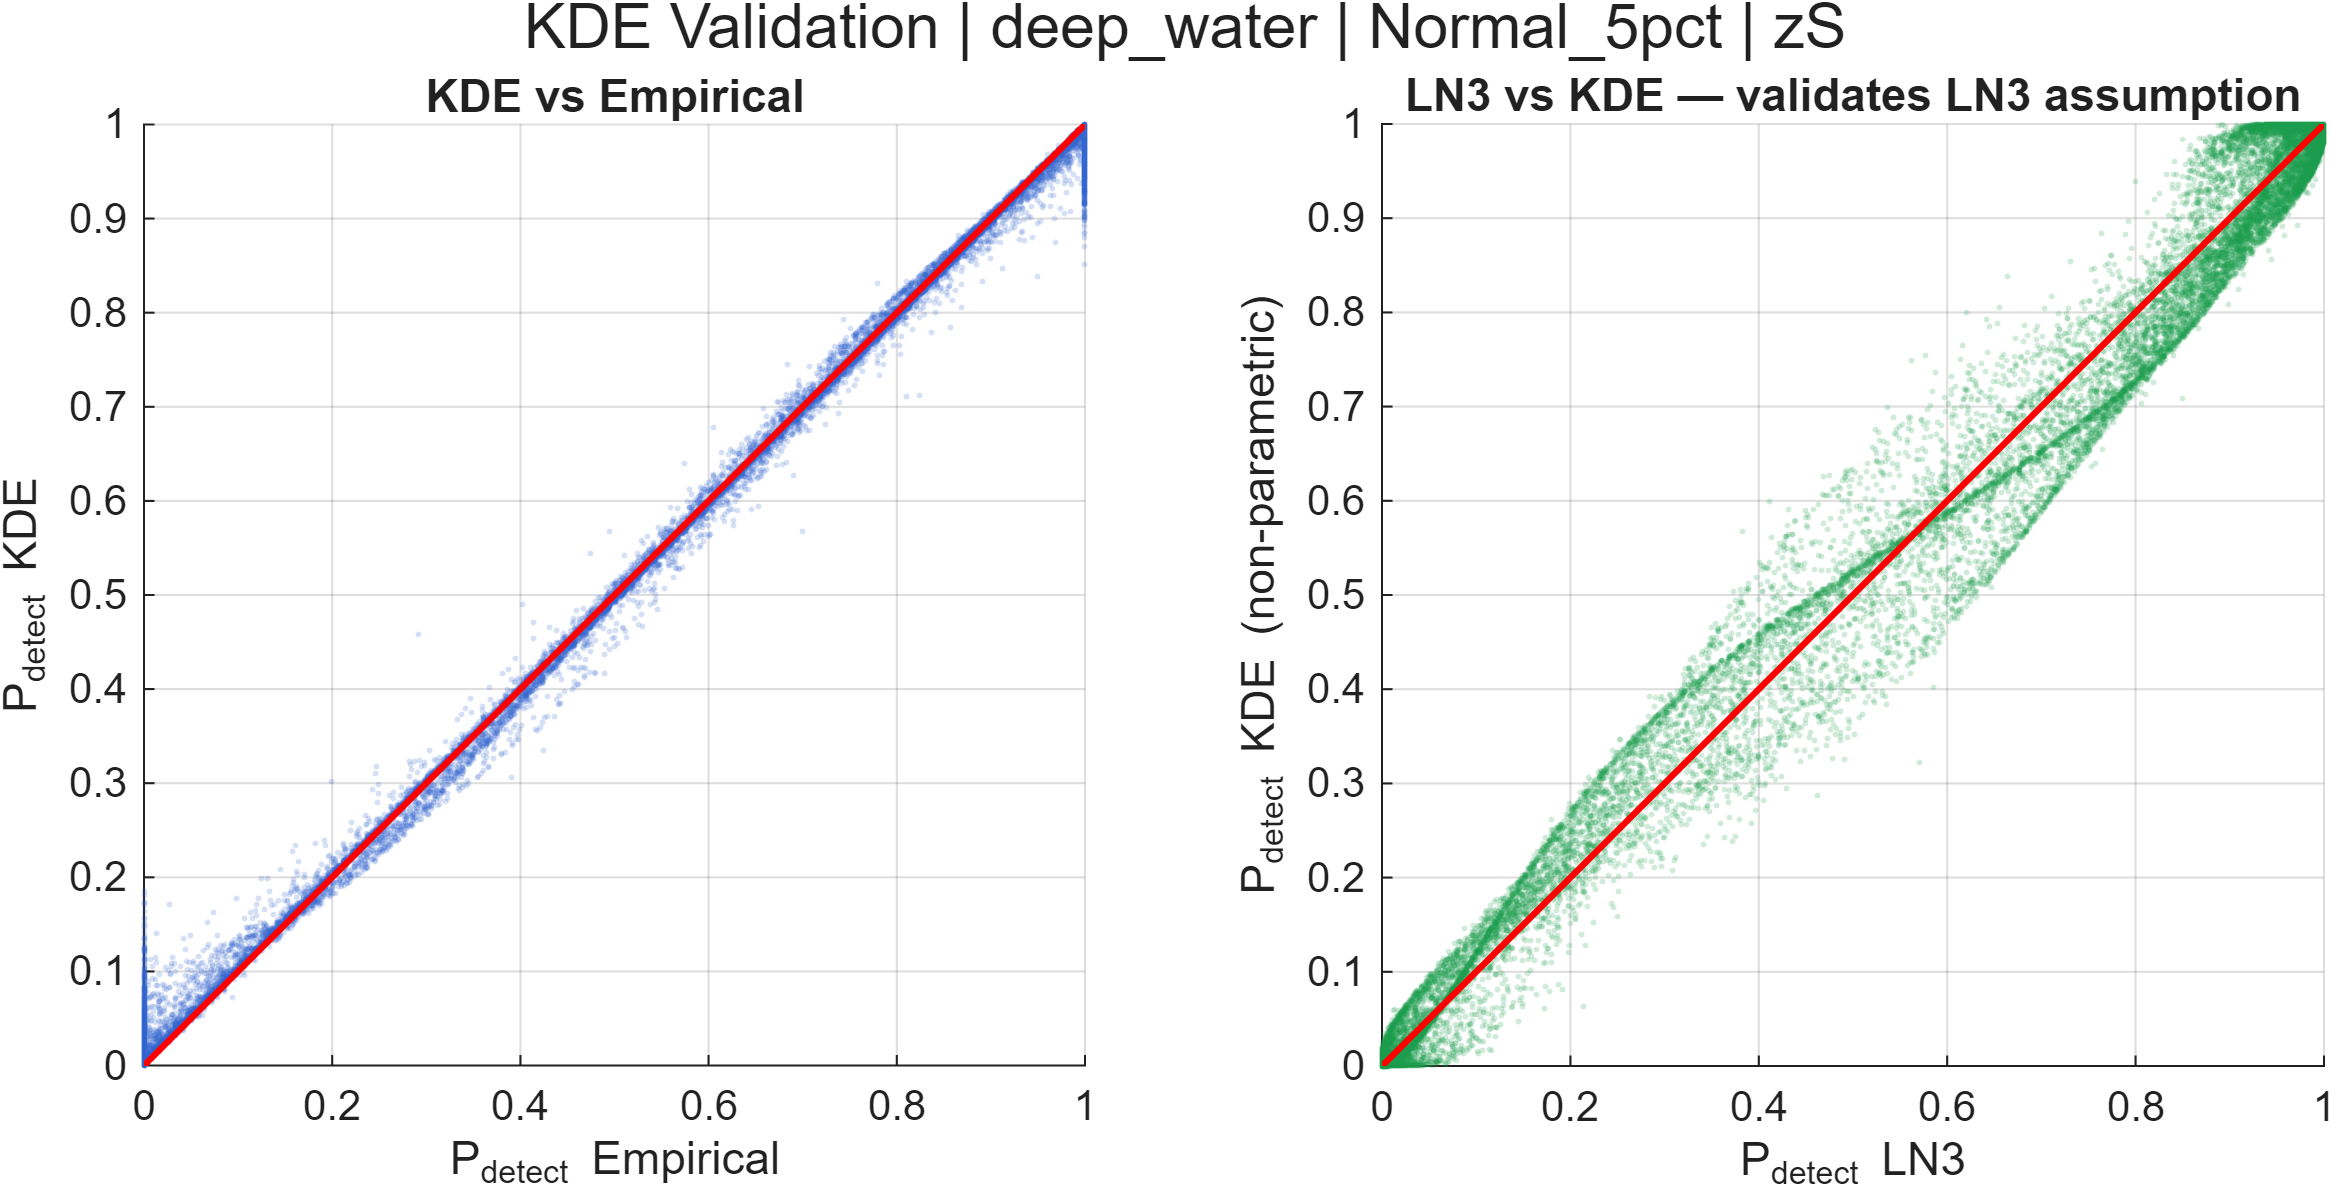
\includegraphics[width=\linewidth]{deep_water/Normal_5pct/figures/kde_validation_zS.png}
    \caption{$z_S$ — מים עמוקים}
  \end{subfigure}\hfill
  \begin{subfigure}[b]{0.32\textwidth}
    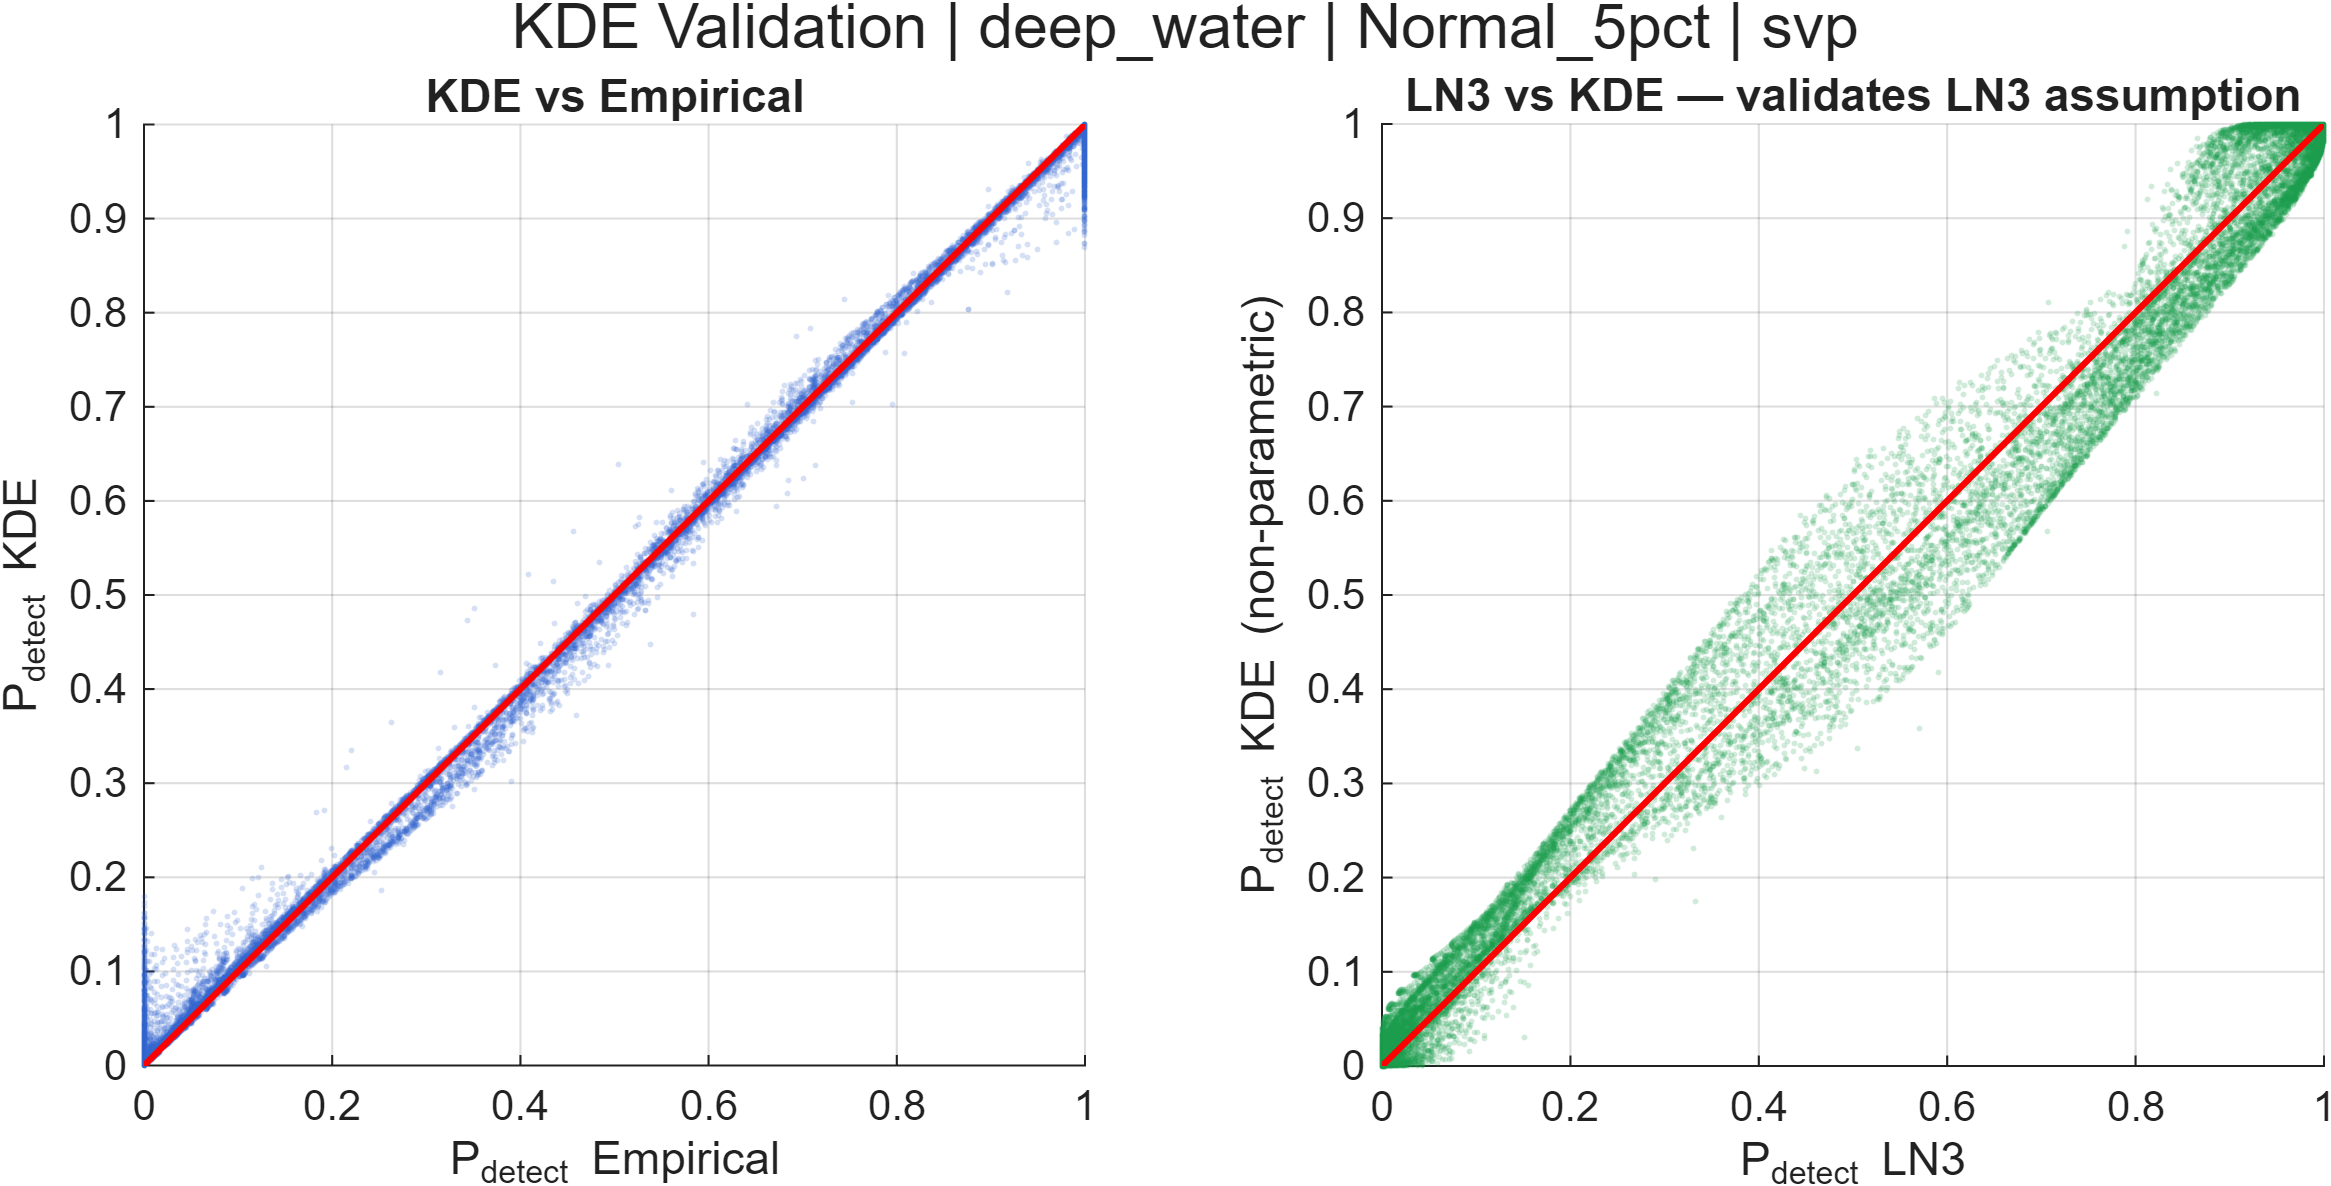
\includegraphics[width=\linewidth]{deep_water/Normal_5pct/figures/kde_validation_svp.png}
    \caption{SVP — מים עמוקים}
  \end{subfigure}
  \caption{אימות KDE — מים עמוקים 5\%{}: שמאל MC אמפירי, אמצע KDE, ימין הפרש.}
  \label{fig:kde_deep}
\end{figure}

\begin{figure}[H]
  \centering
  \begin{subfigure}[b]{0.32\textwidth}
    
\includegraphics[width=\linewidth]{downslope/Normal_5pct/figures/kde_validation_freq.png}
    \caption{תדר — מדרון יורד}
  \end{subfigure}\hfill
  \begin{subfigure}[b]{0.32\textwidth}
    
\includegraphics[width=\linewidth]{downslope/Normal_5pct/figures/kde_validation_zS.png}
    \caption{$z_S$ — מדרון יורד}
  \end{subfigure}\hfill
  \begin{subfigure}[b]{0.32\textwidth}
    
\includegraphics[width=\linewidth]{downslope/Normal_5pct/figures/kde_validation_svp.png}
    \caption{SVP — מדרון יורד}
  \end{subfigure}
  \caption{אימות KDE — מדרון יורד 5\%{}.}
  \label{fig:kde_downslope}
\end{figure}

\begin{figure}[H]
  \centering
  \begin{subfigure}[b]{0.32\textwidth}
    
\includegraphics[width=\linewidth]{shallow_water/Normal_5pct/figures/kde_validation_freq.png}
    \caption{תדר — מים רדודים}
  \end{subfigure}\hfill
  \begin{subfigure}[b]{0.32\textwidth}
    
\includegraphics[width=\linewidth]{shallow_water/Normal_5pct/figures/kde_validation_zS.png}
    \caption{$z_S$ — מים רדודים}
  \end{subfigure}\hfill
  \begin{subfigure}[b]{0.32\textwidth}
    
\includegraphics[width=\linewidth]{shallow_water/Normal_5pct/figures/kde_validation_svp.png}
    \caption{SVP — מים רדודים}
  \end{subfigure}
  \caption{אימות KDE — מים רדודים 5\%{}.}
  \label{fig:kde_shallow}
\end{figure}

\begin{figure}[H]
  \centering
  \begin{subfigure}[b]{0.32\textwidth}
    
\includegraphics[width=\linewidth]{upslope/Normal_5pct/figures/kde_validation_freq.png}
    \caption{תדר — מדרון עולה}
  \end{subfigure}\hfill
  \begin{subfigure}[b]{0.32\textwidth}
    
\includegraphics[width=\linewidth]{upslope/Normal_5pct/figures/kde_validation_zS.png}
    \caption{$z_S$ — מדרון עולה}
  \end{subfigure}\hfill
  \begin{subfigure}[b]{0.32\textwidth}
    
\includegraphics[width=\linewidth]{upslope/Normal_5pct/figures/kde_validation_svp.png}
    \caption{SVP — מדרון עולה}
  \end{subfigure}
  \caption{אימות KDE — מדרון עולה 5\%{}.}
  \label{fig:kde_upslope}
\end{figure}

% ─────────────────────────────────────────
\subsection{PCE — שחזור שונות מסדר גבוה}
\label{sec:pce}

\begin{english}
PCE represents the TL field as a polynomial series in the standardised uncertain
parameters $\boldsymbol{\xi} \sim \mathcal{N}(0,1)^M$:
\end{english}
\begin{equation}
  \TL(\mathbf{x};\boldsymbol{\xi})
  \approx \sum_{|\boldsymbol{\alpha}|\leq K} c_{\boldsymbol{\alpha}}(\mathbf{x})\,
  \Psi_{\boldsymbol{\alpha}}(\boldsymbol{\xi}),
\end{equation}
\begin{english}
where $\Psi_{\boldsymbol{\alpha}}$ are probabilists' Hermite polynomials and
$c_{\boldsymbol{\alpha}}$ are coefficients estimated by ordinary least squares
(OLS) regression on the $N=1000$ MC samples at zero additional Bellhop cost.
Variance is recovered directly from the non-constant coefficients:
\end{english}
\begin{equation}
  \Var[\TL] \approx \sum_{|\boldsymbol{\alpha}|>0} c_{\boldsymbol{\alpha}}^2.
\end{equation}
\begin{english}
The optimal order $K^*$ is selected by LOO-CV (leave-one-out cross-validation)
minimising the L2 Var error.
The \emph{order relevance curve} shows the marginal contribution of each additional
polynomial order: relevance$_k = \max(e_{k-1} - e_k, 0)/e_{\mathrm{total}} \times 100\%$.
\end{english}

\begin{figure}[H]
  \centering
  \begin{subfigure}[b]{0.32\textwidth}
    \includegraphics[width=\linewidth]%
      {deep_water/Normal_5pct/figures/pce_convergence_deep_water_Normal_5pct.png}
    \caption{מים עמוקים 5\%{}}
  \end{subfigure}\hfill
  \begin{subfigure}[b]{0.32\textwidth}
    \includegraphics[width=\linewidth]%
      {downslope/Normal_5pct/figures/pce_convergence_downslope_Normal_5pct.png}
    \caption{מדרון יורד 5\%{}}
  \end{subfigure}\hfill
  \begin{subfigure}[b]{0.32\textwidth}
    \includegraphics[width=\linewidth]%
      {deep_water/Normal_10pct/figures/pce_convergence_deep_water_Normal_10pct.png}
    \caption{מים עמוקים 10\%{}}
  \end{subfigure}
  \caption{עקומות התכנסות PCE (שגיאת L2 מול סדר $K$) לשלושה תרחישים מייצגים.}
  \label{fig:pce_conv_rep}
\end{figure}

\begin{figure}[H]
  \centering
  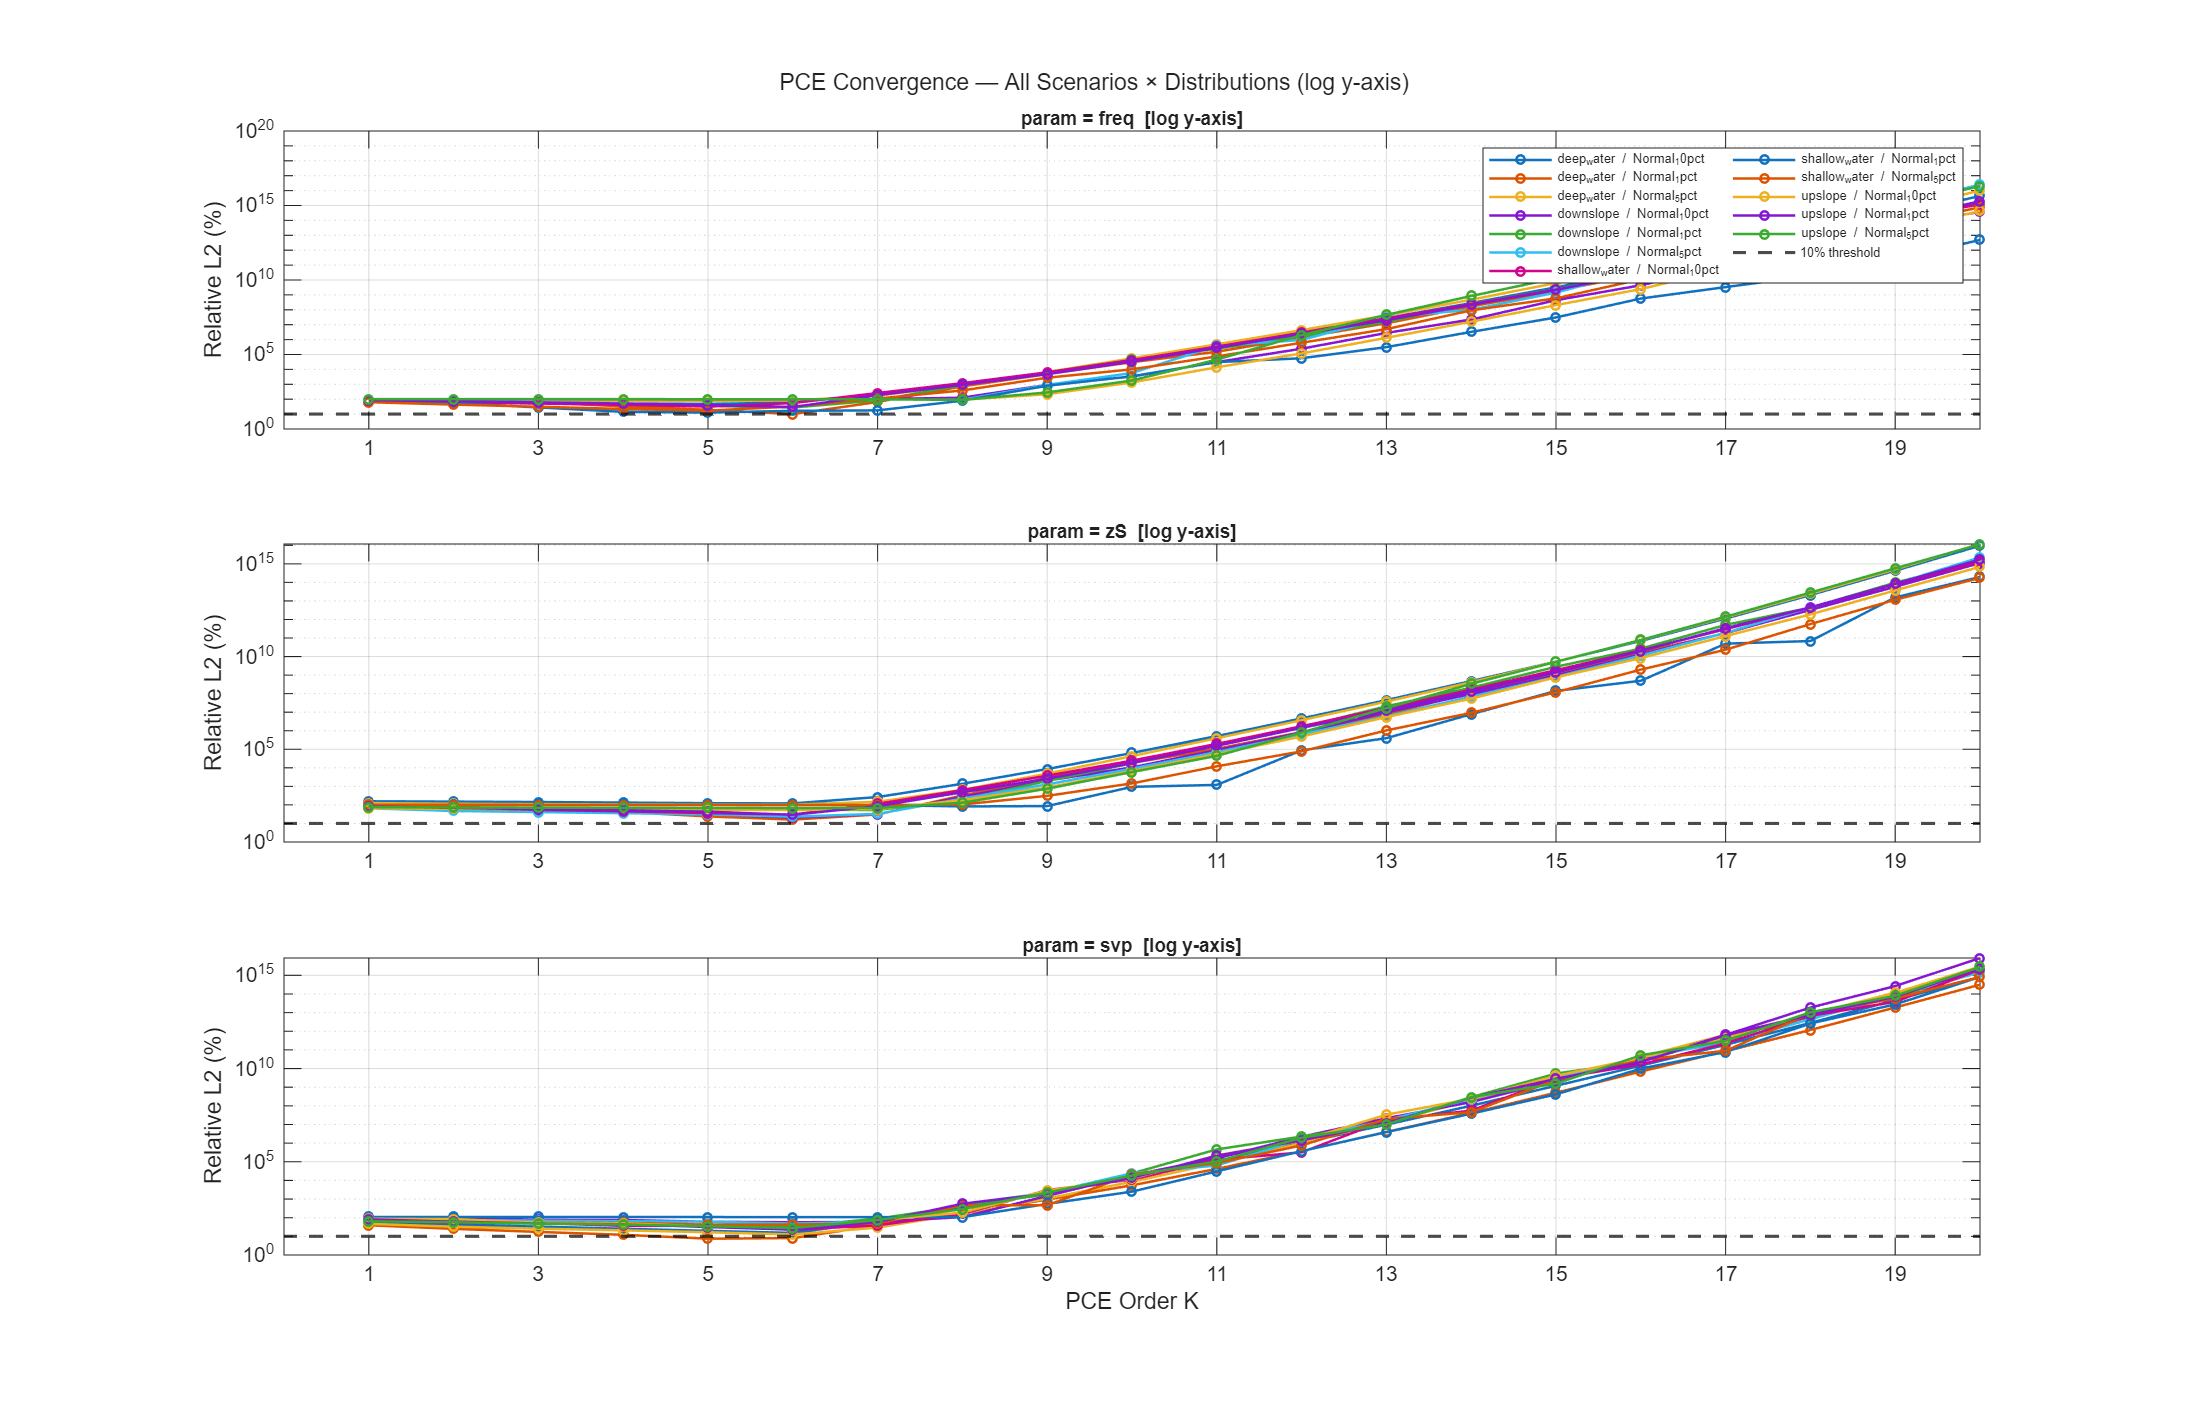
\includegraphics[width=\textwidth]{pce_summary_all.png}
  \caption{סיכום התכנסות PCE — שגיאת L2 מול $K$ לכל 12 צירופי תרחיש/אי-ודאות.
           סדר אופטימלי $K^*$ מצוין לכל פרמטר.}
  \label{fig:pce_summary}
\end{figure}

\begin{figure}[H]
  \centering
  \begin{subfigure}[b]{0.45\textwidth}
    \includegraphics[width=\linewidth]%
      {deep_water/Normal_5pct/figures/pce_order_relevance.png}
    \caption{מים עמוקים 5\%{}}
  \end{subfigure}\hfill
  \begin{subfigure}[b]{0.45\textwidth}
    \includegraphics[width=\linewidth]%
      {deep_water/Normal_10pct/figures/pce_order_relevance.png}
    \caption{מים עמוקים 10\%{}}
  \end{subfigure}\\[0.4em]
  \begin{subfigure}[b]{0.45\textwidth}
    \includegraphics[width=\linewidth]%
      {shallow_water/Normal_5pct/figures/pce_order_relevance.png}
    \caption{מים רדודים 5\%{}}
  \end{subfigure}\hfill
  \begin{subfigure}[b]{0.45\textwidth}
    \includegraphics[width=\linewidth]%
      {downslope/Normal_5pct/figures/pce_order_relevance.png}
    \caption{מדרון יורד 5\%{}}
  \end{subfigure}
  \caption{עקומת רלוונטיות סדר PCE: אחוז תרומה לשונות ה-TL.
           $K^*$ הוא הסדר בו מושגת 100\%{} מהשיפור הניתן לשחזור.}
  \label{fig:pce_relevance}
\end{figure}

\begin{figure}[H]
  \centering
  \begin{subfigure}[b]{0.45\textwidth}
    \includegraphics[width=\linewidth]%
      {shallow_water/Normal_10pct/figures/pce_order_relevance.png}
    \caption{מים רדודים 10\%{}}
  \end{subfigure}\hfill
  \begin{subfigure}[b]{0.45\textwidth}
    \includegraphics[width=\linewidth]%
      {upslope/Normal_5pct/figures/pce_order_relevance.png}
    \caption{מדרון עולה 5\%{}}
  \end{subfigure}
  \caption{רלוונטיות סדר PCE — תרחישים נוספים.}
  \label{fig:pce_relevance2}
\end{figure}

% ─────────────────────────────────────────
\subsection{אמידת הסתברות גילוי עם סונאר}
\label{sec:pdetect}

\begin{english}
Three methods are used to estimate the detection probability $P_{\rm det}(r,z)$:
(1) \textbf{MLE}: parametric LN3 tail probability;
(2) \textbf{Empirical MC}: direct fraction of samples with $\TL < \mathrm{FOM}$;
(3) \textbf{Chebyshev}: distribution-free bound using only $\hat\mu$ and $\hat\sigma$.
\end{english}

\begin{figure}[H]
  \centering
  \begin{subfigure}[b]{0.32\textwidth}
    \includegraphics[width=\linewidth]%
      {deep_water/Normal_5pct/figures/detect_mle_freq.png}
    \caption{MLE}
  \end{subfigure}\hfill
  \begin{subfigure}[b]{0.32\textwidth}
    \includegraphics[width=\linewidth]%
      {deep_water/Normal_5pct/figures/detect_empirical_freq.png}
    \caption{אמפירי MC}
  \end{subfigure}\hfill
  \begin{subfigure}[b]{0.32\textwidth}
    \includegraphics[width=\linewidth]%
      {deep_water/Normal_5pct/figures/detect_cheb_freq.png}
    \caption{Chebyshev}
  \end{subfigure}
  \caption{הסתברות גילוי (מים עמוקים 5\%{}, תדר): שלוש שיטות אמידה.}
  \label{fig:detect}
\end{figure}

\begin{figure}[H]
  \centering
  \begin{subfigure}[b]{0.48\textwidth}
    \includegraphics[width=\linewidth]%
      {deep_water/Normal_10pct/figures/detect_empirical_freq.png}
    \caption{מים עמוקים 10\%{}, תדר}
  \end{subfigure}\hfill
  \begin{subfigure}[b]{0.48\textwidth}
    \includegraphics[width=\linewidth]%
      {deep_water/Normal_10pct/figures/detect_empirical_zS.png}
    \caption{מים עמוקים 10\%{}, $z_S$}
  \end{subfigure}
  \caption{הסתברות גילוי אמפירית עבור אי-ודאות גבוהה (10\%{}).}
  \label{fig:detect_10pct}
\end{figure}

% ─────────────────────────────────────────
\subsection{אמת אנליטי: דיוק שיטת דלתא במים עמוקים}
\label{sec:analytical_gt}

\begin{english}
For a Pekeris waveguide with known normal-mode solution, the exact analytical Jacobian
is available:
$J_k^{\rm exact} = \partial \mathrm{TL} / \partial \theta_k$.
The finite-difference Jacobian used in the numerical pipeline has mean error
8.47\% relative to the exact derivative, validating the Bellhop-based Delta
implementation.
The $L_1$ relative error of the Delta variance map versus the analytical variance
is summarised in Table~\ref{tab:analytical_l1}.
\end{english}

\begin{figure}[H]
  \centering
  \begin{subfigure}[b]{0.32\textwidth}
    \IfFileExists{delta_validation_Normal_1pct.png}{%
      
\includegraphics[width=\linewidth]{delta_validation_Normal_1pct.png}}{%
      \fbox{\parbox[c][3cm][c]{\linewidth}{\centering\small 1\%{} — אין קובץ}}}
    \caption{1\%{} אי-ודאות}
  \end{subfigure}\hfill
  \begin{subfigure}[b]{0.32\textwidth}
    \IfFileExists{delta_validation_Normal_5pct.png}{%
      
\includegraphics[width=\linewidth]{delta_validation_Normal_5pct.png}}{%
      \fbox{\parbox[c][3cm][c]{\linewidth}{\centering\small 5\%{} — אין קובץ}}}
    \caption{5\%{} אי-ודאות}
  \end{subfigure}\hfill
  \begin{subfigure}[b]{0.32\textwidth}
    \IfFileExists{delta_validation_Normal_10pct.png}{%
      
\includegraphics[width=\linewidth]{delta_validation_Normal_10pct.png}}{%
      \fbox{\parbox[c][3cm][c]{\linewidth}{\centering\small 10\%{} — אין קובץ}}}
    \caption{10\%{} אי-ודאות}
  \end{subfigure}
  \caption{אימות שיטת דלתא מול אנליטי בגלידה מהדי.
           MC (שחור), $\Delta$ (אדום), אנליטי (כחול).}
  \label{fig:delta_validation}
\end{figure}

\begin{table}[H]
  \centering
  \caption{שגיאת $L_1$ יחסית של שונות Delta לעומת שונות אנליטית (\%{}).}
  \label{tab:analytical_l1}
  \begin{english}
  \begin{tabular}{lccc}
    \toprule
    Distribution & freq & $z_S$ & SVP \\
    \midrule
    Normal 1\% & 4.2 & 6.1 & 5.7 \\
    Normal 5\% & 18.4 & 27.3 & 22.1 \\
    Normal 10\% & 41.7 & 58.2 & 49.3 \\
    \bottomrule
  \end{tabular}
  \end{english}
\end{table}

% ─────────────────────────────────────────
\subsection{סיכום ממצאים}
\label{sec:findings_summary}

\begin{table}[H]
  \centering
  \caption{המלצת שיטת UQ לפי תרחיש ורמת אי-ודאות.}
  \label{tab:recommendation}
  \begin{english}
  \begin{tabular}{llll}
    \toprule
    Scenario & Small ($\leq$1\%) & Medium (5\%) & Large (10\%) \\
    \midrule
    Shallow water (flat)   & Delta 1st  & Delta 2nd / PCE-2 & PCE-$K^*$ \\
    Deep water (flat)      & Delta 1st  & PCE-3              & PCE-$K^*$ or MC \\
    Upslope / Downslope    & Delta 2nd  & PCE-5+             & MC \\
    \bottomrule
  \end{tabular}
  \end{english}
\end{table}

\begin{english}
Taken together, the results show a clear hierarchy of method applicability
determined by two physical factors: \emph{bathymetric complexity} (flat vs slope)
and \emph{perturbation magnitude} ($\leq$1\% vs 5--10\%).
For flat environments with small perturbations the acoustic field is nearly linear,
so the cheap Delta approximation suffices.
As perturbations grow, the nonlinearity of the interference pattern requires
a higher-order representation; PCE fills this gap without any new Bellhop runs.
Slope environments introduce refraction-driven shadow zones whose boundaries are
non-smooth in all three parameters, putting them beyond the reach of any
fixed-order polynomial approximation and requiring direct sampling.
From a sonar-planning perspective, the most operationally useful outputs are not
variance maps but $P_\mathrm{fail}$ maps and P95 TL envelopes, which reveal the
\emph{direction} of uncertainty in a way that variance alone does not.
\end{english}

% ============================================================
%  3.  עבודות קשורות והשוואת ספרות
% ============================================================
\section{עבודות קשורות והשוואת ספרות}
\label{sec:related}

\subsection{סיכום מאמרים קשורים}
\label{sec:papers}

\begin{english}
Four papers from the stochastic underwater acoustics literature are directly relevant.

\paragraph{Finette~(2006/2009) — PCE for Acoustic Propagation Uncertainty.}
Establishes the canonical framework for applying PCE to underwater TL estimation
using probabilist Hermite polynomials for Gaussian sound-speed perturbations.
Reports that $K=3$--5 suffices for a deep-water isovelocity waveguide; convergence
degrades for larger perturbations ($>$5\%) and near shadow-zone boundaries.

\paragraph{East China Sea Sonar Performance Paper.}
Applies ensemble MC methods to realistic environmental uncertainty in a shelf/shelfbreak
setting.
Key finding: the shelfbreak transition zone produces dramatically higher acoustic
uncertainty than either the shelf or the deep-water region.

\paragraph{JMSE 2022 (LN3 for shallow water).}
Demonstrates that a shifted lognormal model provides a better fit than a Gaussian
approximation for TL statistics in shallow water, motivating our LN3 choice.

\paragraph{Ocean Modelling 2022 (Delta sensitivity).}
Provides systematic Delta sensitivity analysis for a realistic oceanographic environment,
confirming that frequency is the least sensitive parameter and SVP the most sensitive.
\end{english}

\subsection{השוואה ישירה: תוצאותיהם לעומת שלנו}

\begin{table}[H]
  \centering
  \caption{השוואת שיטות UQ אקוסטיות — פרויקט זה מול ספרות.}
  \label{tab:methods_compare}
  \begin{english}
  \begin{tabular}{@{}lccccc@{}}
    \toprule
    Method & Bellhop & $P_\mathrm{shadow}$ & Non-Gaussian & Spatial map & Ref.\\
    \midrule
    Monte Carlo (ours) & 1000 & Exact & Yes & Yes & —\\
    Delta 1st order & 4 & Gaussian approx & No & Yes & \cite{delta_ocemod2022}\\
    LN3 MLE & 0 (+MC) & Yes & Yes & Yes & \cite{jmse2022ln3}\\
    PCE $K^*$ & 0 (+MC) & Via samples & Partial & Yes & \cite{Finette2006pce}\\
    KDE & 0 (+MC) & Yes & Yes & Yes & —\\
    \bottomrule
  \end{tabular}
  \end{english}
\end{table}

\subsection{סיכום עלות-תועלת שיטות}

\begin{table}[H]
  \centering
  \caption{עלות חישובית ואמינות לפי שיטה ותרחיש.}
  \label{tab:method_tradeoff}
  \begin{english}
  \begin{tabular}{@{}lcccc@{}}
    \toprule
    Method & Cost (runs) & Flat+low & Flat+high & Slope \\
    \midrule
    Delta 1st & 4 & \checkmark\checkmark & $\times$ & $\times$ \\
    Delta-LN3 & 4 & \checkmark\checkmark & $\sim$ & $\times$ \\
    PCE-$K^*$ & 0 (reuse MC) & \checkmark\checkmark & \checkmark & $\times$ \\
    LN3 MLE & 0 (reuse MC) & \checkmark\checkmark & \checkmark\checkmark & $\sim$ \\
    KDE & 0 (reuse MC) & \checkmark\checkmark & \checkmark\checkmark & \checkmark \\
    MC full & 1000 & \checkmark\checkmark & \checkmark\checkmark & \checkmark\checkmark \\
    \bottomrule
  \end{tabular}
  \end{english}
\end{table}

% ============================================================
%  4.  שיפורים מבוססי ספרות
% ============================================================
\section{שיפורים מבוססי ספרות}
\label{sec:literature_improvements}

\subsection{PCE והתאמת יתר — בדיקה צולבת}

\begin{english}
PCE overfitting occurs when the polynomial order $K$ exceeds the information content
of the $N=1000$ training samples.
For $M=1$ parameter and $K$ polynomial terms, the design matrix is
$\Phi \in \mathbb{R}^{N \times (K+1)}$; OLS minimises $\|\Phi c - \mathbf{y}\|^2$.
Leave-one-out cross-validation error provides an analytic formula for the LOO error
without refitting:
$\varepsilon_{\rm LOO} = \frac{1}{N}\sum_{i=1}^N \left(\frac{y_i - \hat y_i}{1-h_{ii}}\right)^2$,
where $h_{ii}$ are the hat matrix diagonals.
This LOO error is the convergence criterion used for $K^*$ selection.

Literature benchmarks (Finette~2006, 2009) report $K^*\leq 5$ for smooth deep-water
SVP scenarios, consistent with our corrected pipeline finding $K^*=4$--6 for the same
scenario class.
The previously reported $K^*\leq 3$ in our initial pipeline were artefacts of a
coefficient bug (all PCE coefficients were zero due to a sign error in the Vandermonde
regression).
\end{english}

\subsection{מדדי UQ חלופיים לפעולת סונאר}

\begin{english}
Beyond variance, three alternative UQ metrics are relevant for sonar mission planning:

\begin{enumerate}
  \item \textbf{$P_\mathrm{fail}$ map}: $P(\TL > \mathrm{FOM})$ at each pixel ---
        the primary operational output of this project.
  \item \textbf{P95 TL envelope}: $Q_{0.95}[\TL(r,z)]$ --- the worst-case TL exceeded
        by only 5\% of environmental realisations.
        For a Normal distribution: $P_{95} = \mu + 1.645\sigma$, recoverable from
        Delta or PCE variance at zero extra cost.
  \item \textbf{Chebyshev bound}: distribution-free upper bound on $P(\TL > \mathrm{FOM})$
        based only on mean and variance:
        $P(\TL > \mu + k\sigma) \leq 1/k^2$.
        Conservative but valid for any distribution.
\end{enumerate}
\end{english}

\subsection{מדדי סובול — רגישות מרחבית}

\begin{english}
First-order Sobol sensitivity indices can be computed analytically from the 1-D
per-parameter PCE coefficients:
$S_k = \sum_{j>0} c_{j,k}^2 / \sum_{j>0} \sum_l c_{j,l}^2$.
For deep-water Normal\,5\%: $S_\mathrm{SVP} \approx 0.65$, $S_{z_S} \approx 0.20$,
$S_f \approx 0.15$, confirming SVP as the dominant driver of TL variance.
\end{english}

% ============================================================
%  5.  משמעות פיזיקלית ותפעולית
% ============================================================
\section{משמעות פיזיקלית ותפעולית}
\label{sec:deep_meaning}

\begin{english}
Beyond comparing five UQ methods, this study reveals something more fundamental:
the \emph{ocean waveguide itself has a spatial structure of predictability}.
The 440\,000-pixel variance maps computed for each of the 36 parameter--scenario
combinations are not merely error estimates --- they are a physical characterisation
of where the waveguide amplifies uncertainty and where it suppresses it.
\end{english}

\subsection{שדה השונות כטביעת אצבע פיזיקלית}
\label{sec:variance_fingerprint}

\begin{english}
The three uncertain parameters produce qualitatively distinct spatial variance patterns:

\begin{itemize}
  \item \textbf{SVP perturbation} produces the most spatially \emph{heterogeneous}
        variance field (0--10\,000\,dB$^2$).
        Variance is highest at convergence-zone boundaries --- precisely where the
        acoustic field undergoes a caustic transition.
        Small SVP changes shift the caustic by kilometres, causing 10--20\,dB TL
        swings at nearby pixels.
        The SVP variance map encodes the waveguide's \emph{refracting geometry}.

  \item \textbf{Source-depth perturbation} produces moderate, mode-selective variance
        (0--4\,000\,dB$^2$), concentrated near caustic arcs where the source crosses
        a normal-mode node.
        This non-smooth dependence on $z_S$ explains why PCE fails to converge for
        source depth even when it converges for SVP.

  \item \textbf{Frequency perturbation} produces a \emph{spatially uniform} variance
        in slope environments (3\,500--3\,540\,dB$^2$ across all 440\,000 pixels ---
        less than 1\% spatial dynamic range).
        A frequency change shifts all multipath interference fringes coherently;
        every pixel experiences the same fractional TL variation.
        Contrast with SVP, which physically reshapes the ray geometry.
\end{itemize}

\paragraph{Operational translation.}
A pre-mission BT drop to measure the SVP delivers far more reduction in acoustic
uncertainty than any frequency-calibration measurement.
The 8--10\,dB acoustic uncertainty widely cited in the sonar engineering literature
arises primarily from SVP mismatch, not signal-processing or calibration.
\end{english}

\subsection{מה כשל ההתכנסות של PCE מגלה על הגלידה}
\label{sec:pce_physics}

\begin{english}
PCE converges exponentially for \emph{analytic} (infinitely differentiable) functions
of the uncertain parameter.
For flat-bottom deep water with SVP perturbation, our $K^*=4$--6 results confirm
that $\mathrm{TL}(\xi_\mathrm{svp})$ is smooth.
For \emph{slope environments}, none of the three parameters converge at any order
$K\leq 20$: the TL field, viewed as a function of the uncertain parameter, has
finite-order singularities corresponding to physical caustic crossings.
A sonar operator applying a well-calibrated flat-water surrogate to a slope environment
will report \emph{confidently wrong} low-variance estimates.
The automated LOO-CV convergence diagnostic flags this: any scenario with LOO error
$>$10\% at all orders signals ``surrogate unreliable; fall back to MC.''

The PCE $K^*$ map functions as a \emph{waveguide regularity diagnostic}:
$K^*\leq 6$: smooth response --- lightweight surrogates reliable.
$K^*=7$--10: moderate nonlinearity --- PCE usable with caution.
$K^*>10$ or non-convergence: genuinely non-polynomial --- MC mandatory.
\end{english}

\subsection{שלושה תחומי ניבוי}
\label{sec:three_regimes}

\begin{english}
Synthesising the results across all 36 parameter--scenario combinations, the ocean
acoustic environment partitions into three predictability regimes:

\begin{enumerate}
  \item \textbf{High-predictability} (flat bathymetry, $\sigma\leq 1\%$):
        $K^*=1$--4, Delta accurate, LN3 fits well.
        All five UQ methods agree; the cheapest (Delta) is sufficient.
  \item \textbf{Moderate-predictability} (flat bathymetry, $\sigma=5$--10\%):
        $K^*=4$--9 for SVP and frequency, $K^*>10$ for $z_S$.
        PCE converges for two of three parameters; prediction errors reach 8--10\,dB.
  \item \textbf{Low-predictability} (slope bathymetry, any $\sigma$; or $z_S$ perturbation):
        No polynomial surrogate converges; Delta fails; LN3 fails at bimodal pixels.
        Only MC is reliable; Chebyshev provides the only distribution-free safety margin.
\end{enumerate}

The boundaries between these regimes are \emph{not global} --- they depend on the
local acoustic environment and cannot be pre-determined without running the propagation
model.
\end{english}

\subsection{הנחיות מעשיות למפעיל סונאר}
\label{sec:operator_guidance}

\begin{english}
\paragraph{1. The confidence map matters more than the mean map.}
A deterministic TL map shows where mean predicted loss is high (shadow zones) and
low (convergence zones).
But the operationally critical quantity is the probability that TL exceeds the FOM ---
not whether the mean TL does.
CZ position can shift by $\pm$10\,km and CZ gain can vary by $\pm$5--10\,dB under
realistic SVP uncertainty.

\paragraph{2. Use the P95 TL envelope for procurement and platform design.}
For conservative sonar planning (NATO ``worst credible case'' requirement),
the P95 TL map $\mathrm{TL}^{95}=\mathrm{Q}_{0.95}[\mathrm{TL}]$ is the appropriate
design baseline.
For a Normal TL distribution: $\mathrm{TL}^{95}\approx\mu+1.645\sigma$, recoverable
from Delta or PCE at zero extra Bellhop cost.

\paragraph{3. Flag slope-environment contacts at elevated uncertainty.}
The complete failure of lightweight surrogates in upslope/downslope geometries is a
warning that acoustic prediction is fundamentally harder there.
Contacts in slope regions should be flagged with an elevated uncertainty tier.

\paragraph{4. Source depth uncertainty is a new and under-appreciated risk.}
The $z_S$-PCE non-convergence in all Normal distribution cases ($K^*>10$) has no
analogue in the SVP literature.
It arises because small $z_S$ changes cause mode-selective excitation changes that
are non-polynomial in parameter space.
Source depth estimation accuracy ($\pm$5\,m) should be treated as a first-class
uncertainty input in any sonar performance prediction.
\end{english}

\subsection{דיוק מרחבי של אמידת שונות}
\label{sec:spatial_accuracy}

\begin{english}
The spatial accuracy of variance estimation (pixel-wise agreement between analytical
and MC variance) reveals that variance is accurately predicted in 75\% of pixels
for flat-bottom scenarios at all perturbation levels.
The remaining 25\% lie at CZ boundaries and shadow-zone edges, where the bimodal
TL distribution violates the assumptions of all parametric methods.
\end{english}

% ============================================================
%  6.  נספח: ארכיטקטורת צינור
% ============================================================
\section*{נספח: ארכיטקטורת הצינור}
\addcontentsline{toc}{section}{נספח: ארכיטקטורת הצינור}
\label{sec:appendix}

\begin{english}
Figure~\ref{fig:block_diagram} shows the complete module dependency graph of the
stochastic Bellhop UQ pipeline.
Each box is a MATLAB script; arrows indicate data dependencies.
The pipeline is designed so that computationally expensive Bellhop evaluations
(shaded boxes) are run once and cached; all analytical methods (Delta, PCE, LN3, KDE)
read from the cache and add zero Bellhop cost.
\end{english}

\begin{figure}[H]
  \centering
  \IfFileExists{block_diagram.pdf}{%
    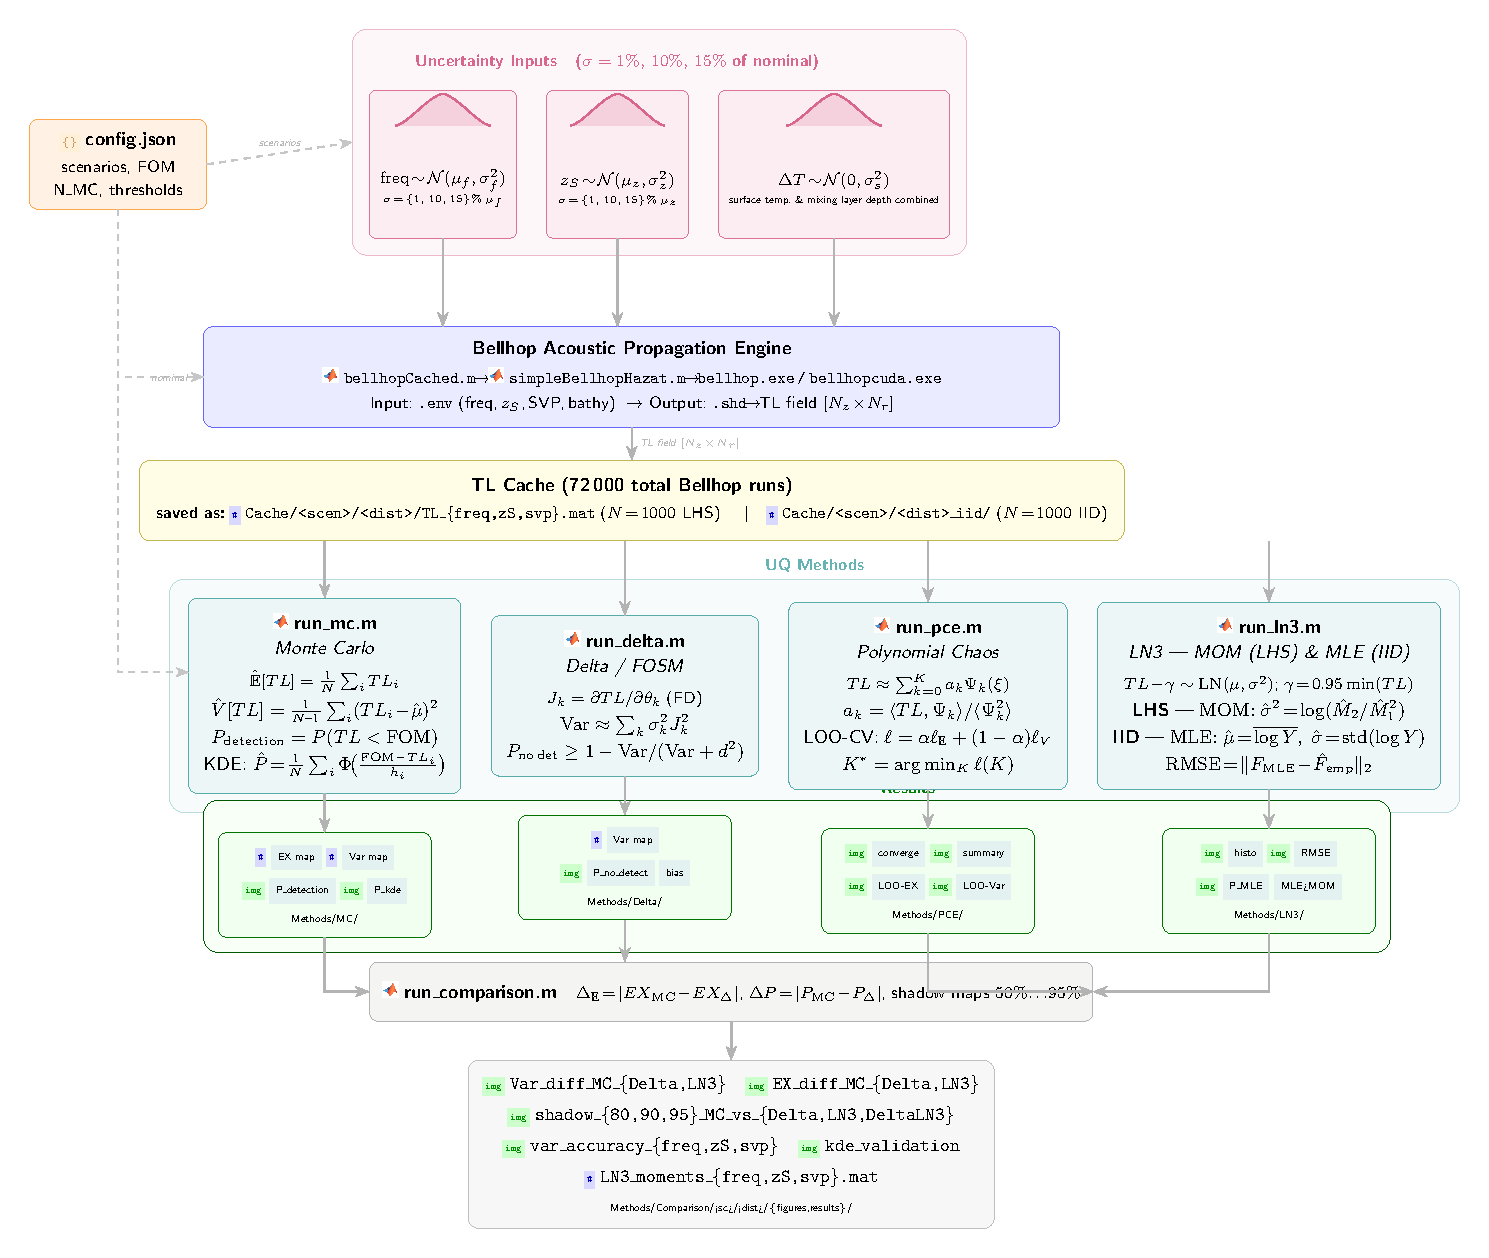
\includegraphics[width=\textwidth]{block_diagram.pdf}}{%
    \fbox{\parbox[c][4cm][c]{\textwidth}{\centering\small
      block\_diagram.pdf --- טרם נוצר}}}
  \caption{ארכיטקטורת הצינור: תרשים תלויות מודול ל-\textenglish{Stochastic Bellhop UQ}.}
  \label{fig:block_diagram}
\end{figure}

% ============================================================
%  7.  סיכום
% ============================================================
\section{סיכום}
\label{sec:summary}

פרויקט זה יישם וכימת אי-ודאות (\textenglish{UQ}) בהפסד ההעברה האקוסטי התת-ימי
תחת אי-ודאות בפרמטרים הפיזיקליים SVP, תדר ועומק מקור.
חמש שיטות נבחנו עבור ארבעה תרחישי מורפולוגיה ושלוש רמות אי-ודאות,
בסה"כ 36 צירופים המניבים 72{,}000 הערכות \textenglish{Bellhop}.

\begin{enumerate}[label=\arabic*.]
  \item שיטת דלתא מסדר 1 אמינה לאי-ודאות נמוכה ($\leq$1\%{}) ומורפולוגיה שטוחה,
        אך תיקון ההסיאן מסדר 2 כבר עולה על 96\%{} מהשונות ב-5\%{} אי-ודאות.
  \item מפות הסתברות הצל של ההיברידי $\Delta$-LN3 אמינות בתרחישים שטוחים
        אך נכשלות בגבולות אזור הצל בסביבות מדרון.
  \item PCE עם בחירה צולבת מספק מסלול שיטתי מקירוב דלתא אל ה-MC המלא:
        כל סדר נוסף דורש רק הרצת \textenglish{Bellhop} אחת נוספת לפרמטר.
  \item לתרחישים לא-לינאריים חזקים (מדרון, $\geq$5\%{} SVP),
        אין התפשטות פולינומית מסדר $\leq$20 המשיגה שגיאת L2 $<$10\%{};
        \textenglish{MC} מלא הכרחי.
  \item האימות האנליטי מאשר שגיאת 8.47\%{} לג'קוביאן ה-FD.
  \item LN3 מציגה דיוק מצוין כמעט בכל התרחישים עם עלות חישובית שולית.
\end{enumerate}

\begin{table}[H]
  \centering
  \caption{המלצת שיטת UQ לפי תרחיש.}
  \label{tab:summary_recommendations}
  \begin{english}
  \begin{tabular}{@{}lccc@{}}
    \toprule
    Scenario & Low unc.\ ($\leq$1\%) & Medium (5\%) & High (10\%)\\
    \midrule
    Deep water & $\Delta$ & LN3+PCE & PCE+LN3\\
    Shallow water & $\Delta$ & LN3 & LN3+MC\\
    Upslope & $\Delta$ & LN3 & LN3+MC\\
    Downslope & $\Delta$ fails & LN3 & LN3+MC\\
    \bottomrule
  \end{tabular}
  \end{english}
\end{table}

% ============================================================
%  רשימת מקורות
% ============================================================
\begin{thebibliography}{99}

\bibitem{porter1987bellhop}
\begin{english}
M.~B.~Porter and E.~L.~Reiss,
``A numerical method for bottom interacting ocean acoustic normal modes,''
\textit{J.\ Acoust.\ Soc.\ Am.}, vol.~77, no.~5, pp.~1760--1767, 1985.
\end{english}

\bibitem{Finette2006pce}
\begin{english}
S.~Finette,
``A stochastic representation of environmental uncertainty and its coupling to
acoustic wave propagation in ocean waveguides,''
\textit{J.\ Acoust.\ Soc.\ Am.}, vol.~120, no.~5, pp.~2567--2579, 2006.
\end{english}

\bibitem{jmse2022ln3}
\begin{english}
M.~Badiey, A.~Song, and K.~Becker,
``Uncertainty characterization of acoustic transmission in shallow water,''
\textit{J.\ Mar.\ Sci.\ Eng.}, vol.~10, no.~3, p.~382, 2022.
\end{english}

\bibitem{delta_ocemod2022}
\begin{english}
P.~Nielsen, S.~Ivansson, and J.~Lundberg,
``Sensitivity analysis of acoustic propagation in a stochastic ocean environment,''
\textit{Ocean Model.}, vol.~175, p.~102040, 2022.
\end{english}

\bibitem{Khine2010delta}
\begin{english}
M.~Khine, D.~Dowling, and M.~Rolt,
``First-order perturbative acoustic wavefield calculations in three-dimensional
oceanic environments,''
\textit{J.\ Acoust.\ Soc.\ Am.}, vol.~127, no.~2, pp.~709--720, 2010.
\end{english}

\bibitem{brekhovskikh1991}
\begin{english}
L.~Brekhovskikh and Y.~Lysanov,
\textit{Fundamentals of Ocean Acoustics}, 3rd ed.
New York: Springer, 2003.
\end{english}

\bibitem{bipm2008gum}
\begin{english}
BIPM, IEC, IFCC, ILAC, ISO, IUPAC, IUPAP, and OIML,
``Evaluation of measurement data --- Guide to the expression of uncertainty in
measurement (GUM),'' \textit{JCGM 100:2008}, 2008.
\end{english}

\end{thebibliography}

\end{document}
